\documentclass[10pt,aspectratio=169]{beamer}

\usetheme{lisn}
\usepackage[utf8]{inputenc}
\usepackage[T1]{fontenc}
\usepackage{appendixnumberbeamer}
\usepackage{url}
\usepackage{booktabs}
\usepackage[scale=2]{ccicons}
\usepackage{amsfonts}
\usepackage{amssymb}
\usepackage{amsmath}
\newcommand{\largehline}{\specialrule{.16em}{.3em}{.3em}}
\newcommand{\mediumhline}{\specialrule{.10em}{.2em}{.2em}}
\usepackage{pgfplots}

\usepackage{multirow}
\usepackage{graphicx}
%\usepackage{sidecap}


\usepackage{xspace}
\newcommand{\themename}{\textbf{\textsc{lisn}}\xspace}


\title{Dialogue Systems And Evaluation}
\subtitle{\textbf{}}
\date{\today}
\author{Thomas Gerald}

\institute{Laboratoire Interdisciplinaire des Sciences du Numérique -- LISN, CNRS\\\texttt{firstname.lastname@lisn.upsaclay.fr}}
\titlegraphic{\centering
\includegraphics[height=1.2cm]{img/LISN-LOGO-JPG-Quadri-edition-S.jpg}  \hfill 
\includegraphics[height=1.0cm]{img/LOGO_CNRS_2019_RVB.png}  
\includegraphics[height=1.0cm]{img/Logotype-UPSaclay_CMJN.jpg}}
\begin{document}

\maketitle
\section{Objectives of the course}
\begin{frame}{Objectives : The Lesson}
    \begin{columns}
        \begin{column}{0.5\textwidth}
            \begin{block}{Overview of Dialogue systems:}
                \begin{itemize}
                    \item \textbf{What is a dialogue system?} Provide definitions to understand the differents aspect of dialogue systems.
                    \item \textbf{How does it works?} Define the main objectives and the structure of the different approaches
                    \item \textbf{What is the current state of the art and what next?} Provide a short overview of futures directions to better adress conversation tasks
                \end{itemize}
            \end{block}
        \end{column}
        \begin{column}{0.5\textwidth}
            \begin{block}{Corpus \& Evaluation: }
                \begin{itemize}
                    \item \textbf{What kind of data?} Overview of dialogue corpus
                    \item \textbf{How to evaluate? } Presentation of the different evaluation approaches 
                \end{itemize}
            \end{block}
            \begin{alertblock}{What it is not covered here?}
                Details on all the approaches. 
            \end{alertblock}
        \end{column}
    \end{columns}
\end{frame}
\begin{frame}{Objectives : Application (and homework)}
    \begin{columns}
        \begin{column}{0.5\textwidth}
            \begin{figure}
                \centering
                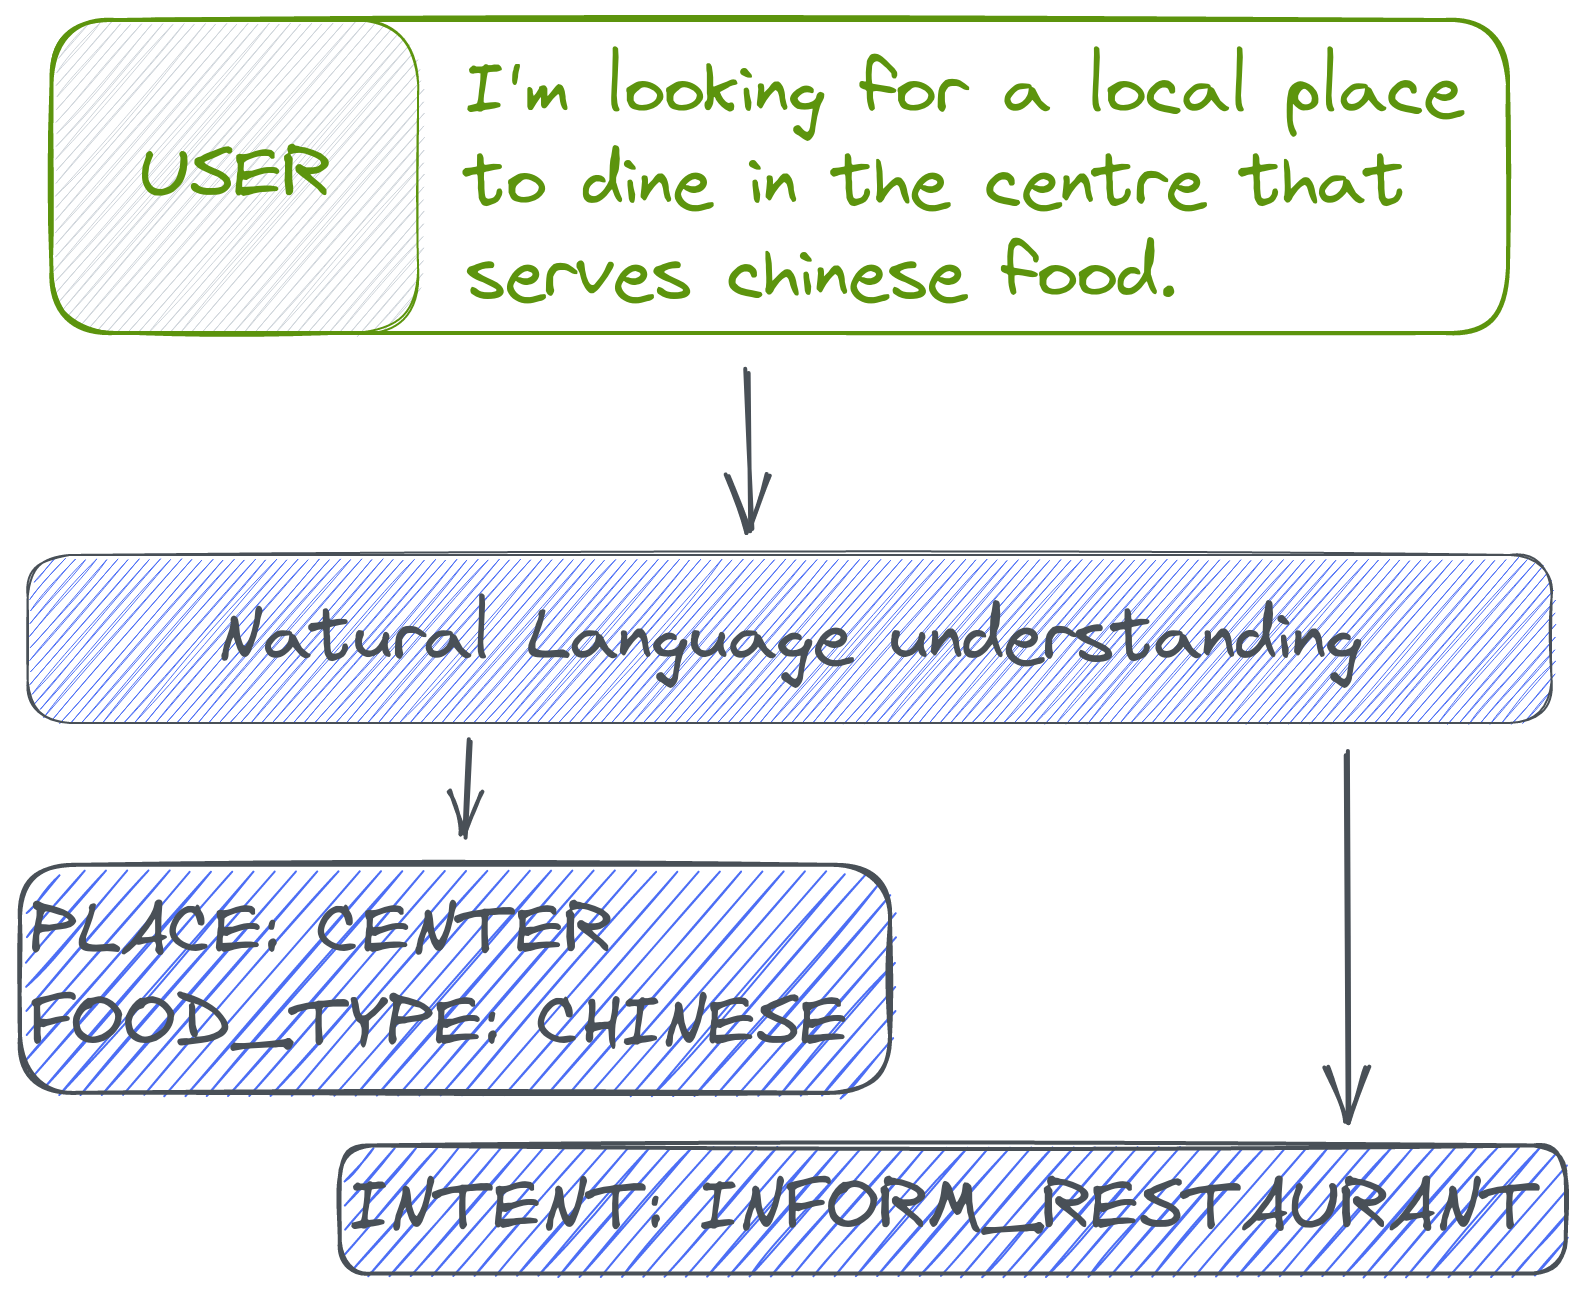
\includegraphics[width=.9\textwidth]{media/TP-exemple.png}
            \end{figure}
        \end{column}
        \begin{column}{0.5\textwidth}
            \begin{block}{A task oriented system for restaurant booking:}
                \begin{itemize}
                    \item Build a simple NLU model (we will explain it later)
                    \item Evaluate the different approaches
                    
                \end{itemize}
            \end{block}
        \end{column}
    \end{columns}
\end{frame}


\section{introduction}
\begin{frame}{Introduction}
    \begin{columns}
        \begin{column}{0.5\textwidth}
            \begin{block}{Objectives of a Dialogue Systems}
                \begin{itemize}
                    \item Provide a service to help users to fullfill a task 
                        \begin{itemize}
                            \item Specific knowledge (e.g. medical, gathering informations, FAQ)
                            \item Interact to complete a task with real world implication (e.g. booking, agenda etc..)
                        \end{itemize}
                    \item Interract with the user in a sequential ways (dialogue)
                    \item Interract in natural language
                 \end{itemize}
            \end{block}
        \end{column}
        \begin{column}{0.5\textwidth}
            \begin{block}{Different terms  for dialogue systems}
                \begin{itemize}
                    \item Conversationnal agent : implies an avatar (animated agent)
                    \item Dialogue System : interract with a system  (e.g. knowledge base, relationnal database...)
                    \item Chatbots and intelligent assistant : more often used from application point of view
                \end{itemize}
            \end{block}
        \end{column}
    \end{columns}
\end{frame}

\begin{frame}{Dialogue systems}
    \begin{columns}
        \begin{column}{0.5\textwidth}
            \begin{block}{Define two actors}
                \begin{itemize}
                    \item \textbf{USER:} An user (person) which interact with the system. The user query the System. 
                    \item \textbf{SYSTEM:} The chatBot system detect the intent of the user and answer accordingly 
                \end{itemize}
            \end{block}
            \begin{block}{Concept definition}
                \begin{itemize}
                    \item \textbf{utterance:} text of a turn weither by user or the system
                    \item \textbf{user intent:} intention given by the user (must be interpreted by the model)
                \end{itemize}
            \end{block}
        \end{column}
        \begin{column}{0.5\textwidth}
            \begin{figure}
                \centering
                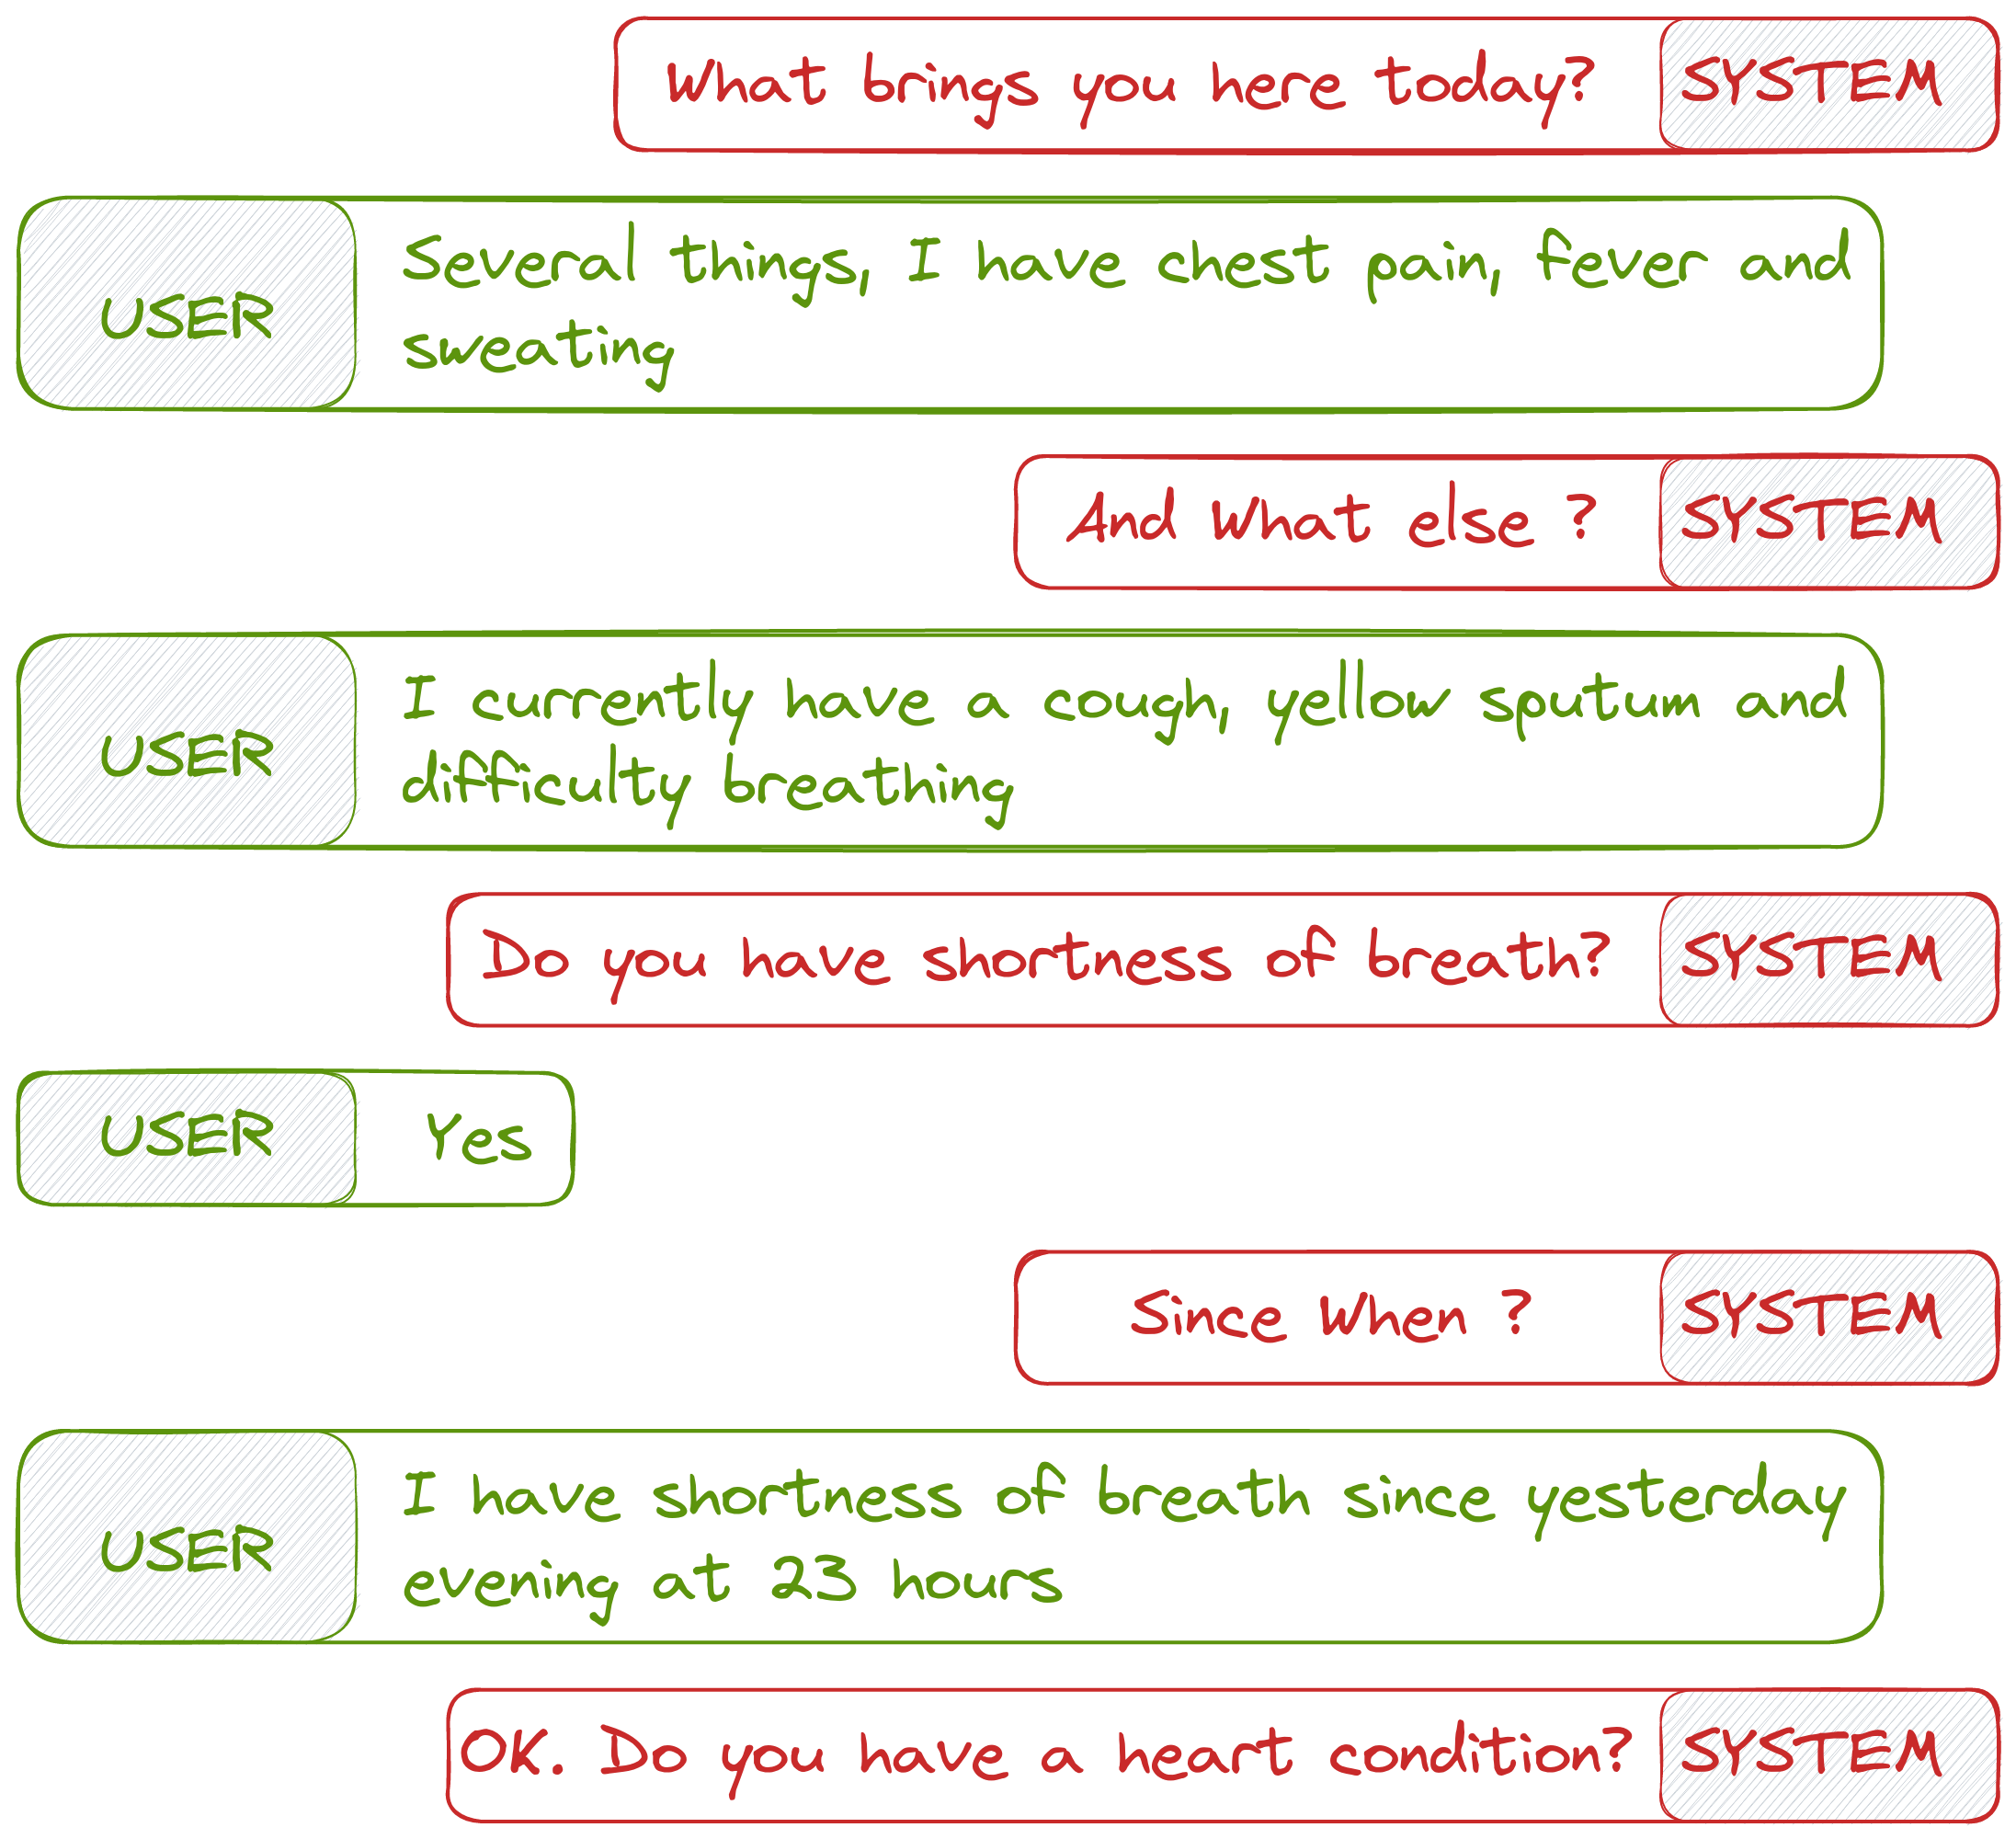
\includegraphics[width=.9\textwidth]{media/dialogue_patient.png}
                \caption{An example of dialogue in PVDial corpus}
                \label{fig:example-pvdial}
            \end{figure}
        \end{column}
    \end{columns}
\end{frame}

\begin{frame}{Dialogue systems : basics}
    \begin{columns}
        \begin{column}{0.5\textwidth}
            \begin{figure}
                \centering
                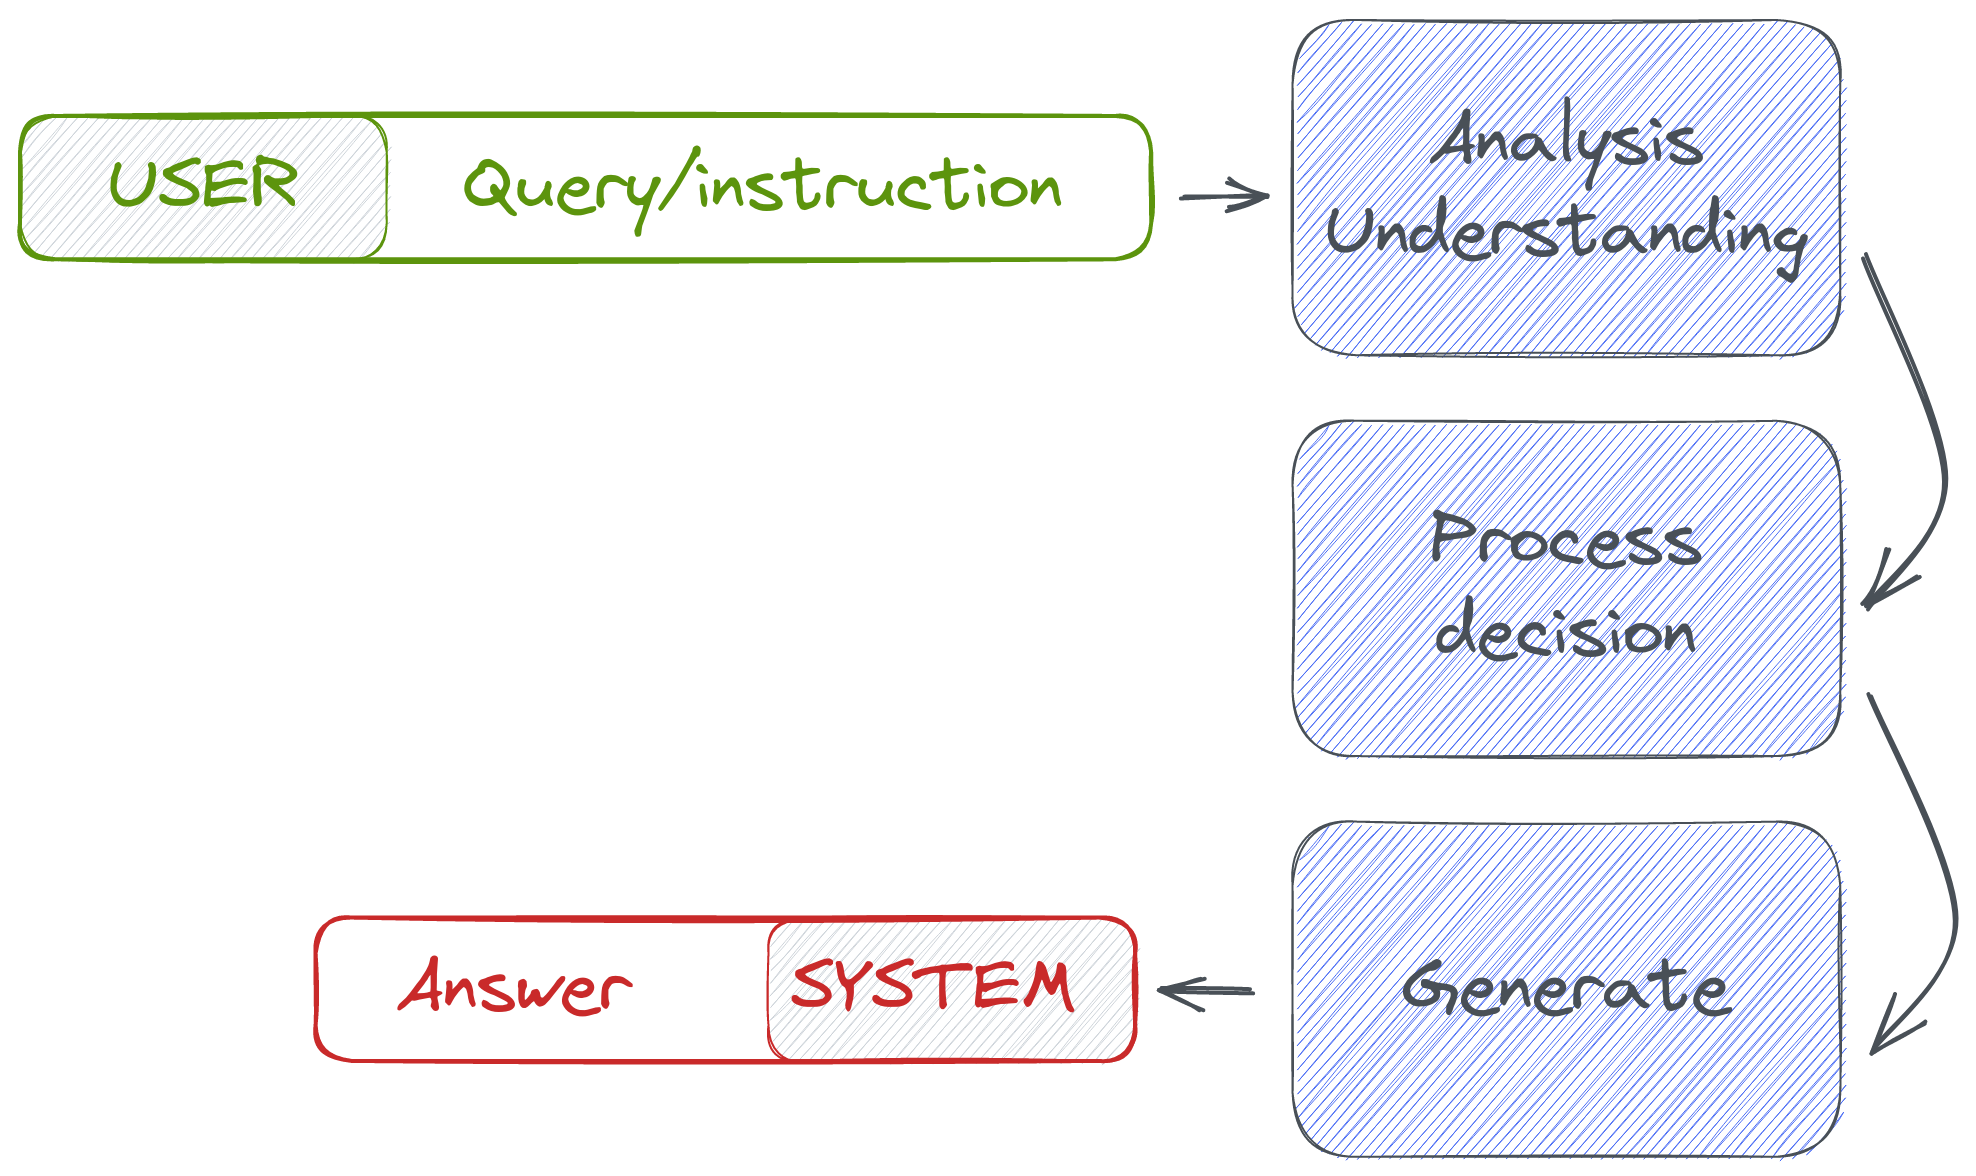
\includegraphics[width=1.\textwidth]{media/base_process_dial.png}
                \caption{Base concepts of a Dialogue system }
                \label{fig:base-process}
            \end{figure}
        \end{column}
        \begin{column}{0.5\textwidth}
            \begin{block}{A simple dialogue system: }
                \begin{itemize}
                    \item \textbf{Analyse:} Analysing the user utterence to understant the user intent
                    \item \textbf{Act/decide:} Select an action (e.g. query a database), next information to return(inform/clarify)
                    \item \textbf{Generate:} Return textual information about action/requeste of the users
                \end{itemize}

                \begin{block}{Needs: }
                    \begin{itemize}
                        \item A combination of different systems (not always true, e.g. end-to-end system)
                        \item Cover at least two differents objectives,  accomplish a task and chat with user
                    \end{itemize}
                \end{block}
            \end{block}
        \end{column}
    \end{columns}
\end{frame}


\begin{frame}{Chatbot different approaches}

            \begin{block}{Different  kind of systems: }
                \begin{itemize}
                    \item \textbf{Task-oriented systems:} Help user to fullfill a task, obtain information on a specific topic such as booking restaurant, specific medical advice...
                    \item \textbf{ChitChat/purely conversational systems:} Finding the most natural reaction to an user utterance and maintain engagement
                    \item \textbf{Question-answering systems:} Help the user to find informations or answers to a question (it can be document/facts or generated answers)
                \end{itemize}
            \end{block}
            All those objectives can be combined !!!

\end{frame}

\section{Task Oriented Dialogue systems}
\begin{frame}
    \begin{figure}[t]
        \centering
        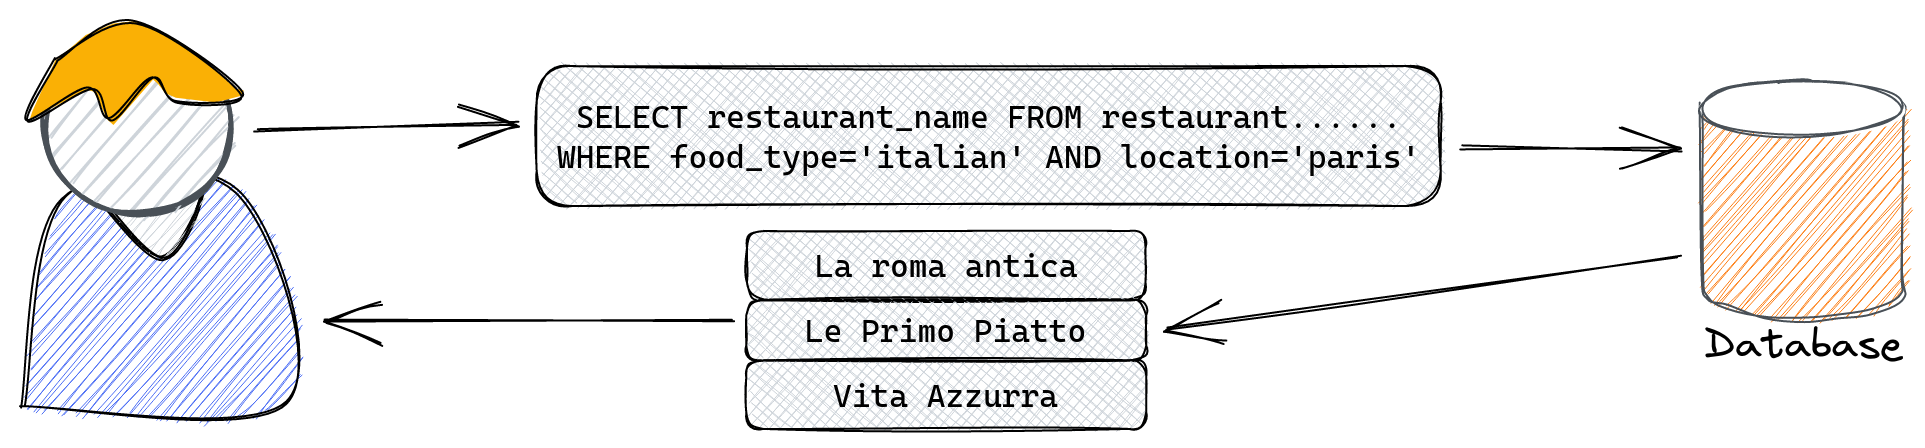
\includegraphics[width=.9\textwidth]{media/task-dial-2.png}
    \end{figure}
    \begin{columns}
        \begin{column}{0.5\textwidth}
            \begin{block}{Query a database:}
                \begin{itemize}
                    \item Query to get information from a database
                    \item Update the database (e.g. to book a reservation, register task in an agenda...)
                \end{itemize}
            \end{block}
        \end{column}
        \begin{column}{0.5\textwidth}
            \begin{alertblock}{Drawback}
                Not easy to interract  for most people (and in all case it is time consuming)
            \end{alertblock}
        \end{column}
    \end{columns}
\end{frame}

\begin{frame}
    \begin{figure}[t]
        \centering
        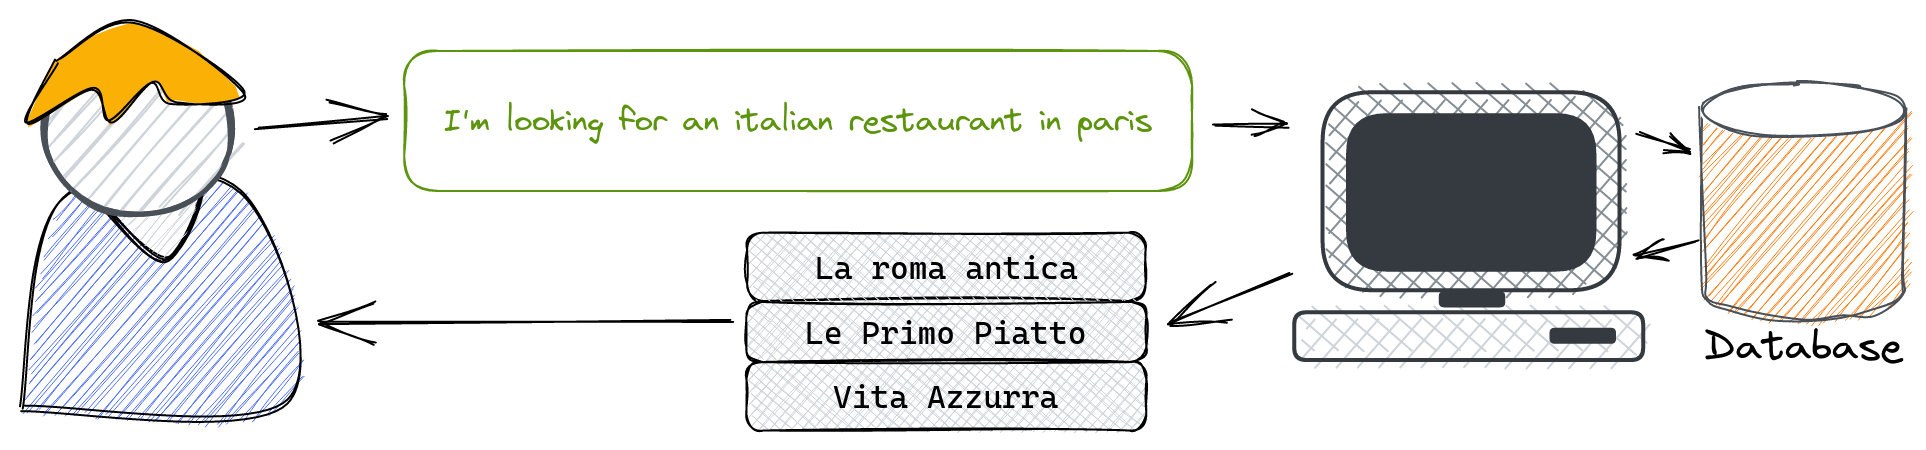
\includegraphics[width=.9\textwidth]{media/task-dial-3.png}
    \end{figure}
    \begin{columns}
        \begin{column}{0.5\textwidth}
            \begin{block}{Query the system:}
                \begin{itemize}
                    \item Query the system in natural language (NLU system) 
                    \item The system will ``transform''the query into database instruction
                \end{itemize}
            \end{block}
        \end{column}
        \begin{column}{0.5\textwidth}
            \begin{alertblock}{Drawback}
                Answer can be difficult to interpret
            \end{alertblock}
        \end{column}
    \end{columns}
\end{frame}
\begin{frame}
    \begin{figure}[t]
        \centering
        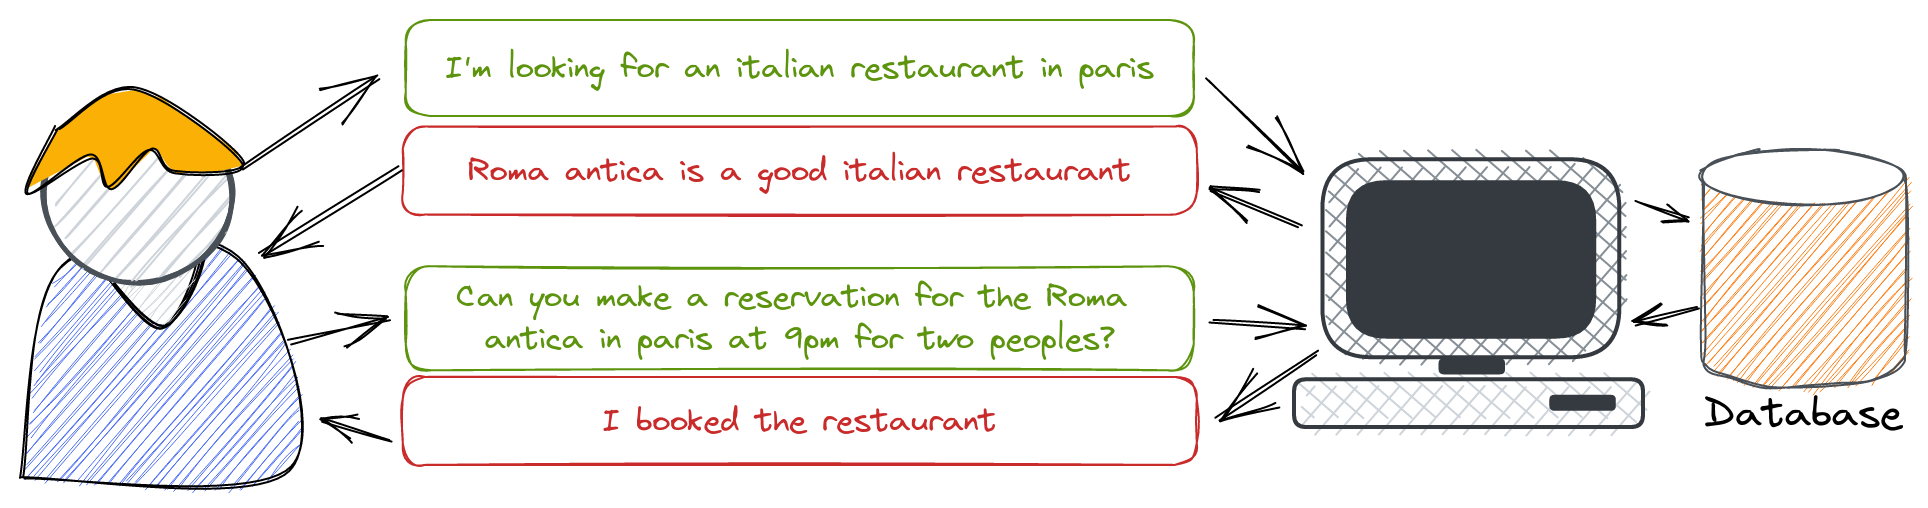
\includegraphics[width=.9\textwidth]{media/task-dial-4.png}
    \end{figure}
    \begin{columns}
        \begin{column}{0.5\textwidth}
            \begin{block}{System Answer}
                \begin{itemize}
                    \item Translate the responses in natural language
                \end{itemize}
            \end{block}
        \end{column}
        \begin{column}{0.5\textwidth}
            \begin{alertblock}{Drawback}
               Not able to understand context
            \end{alertblock}
        \end{column}
    \end{columns}
\end{frame}
\begin{frame}
    \begin{figure}[t]
        \centering
        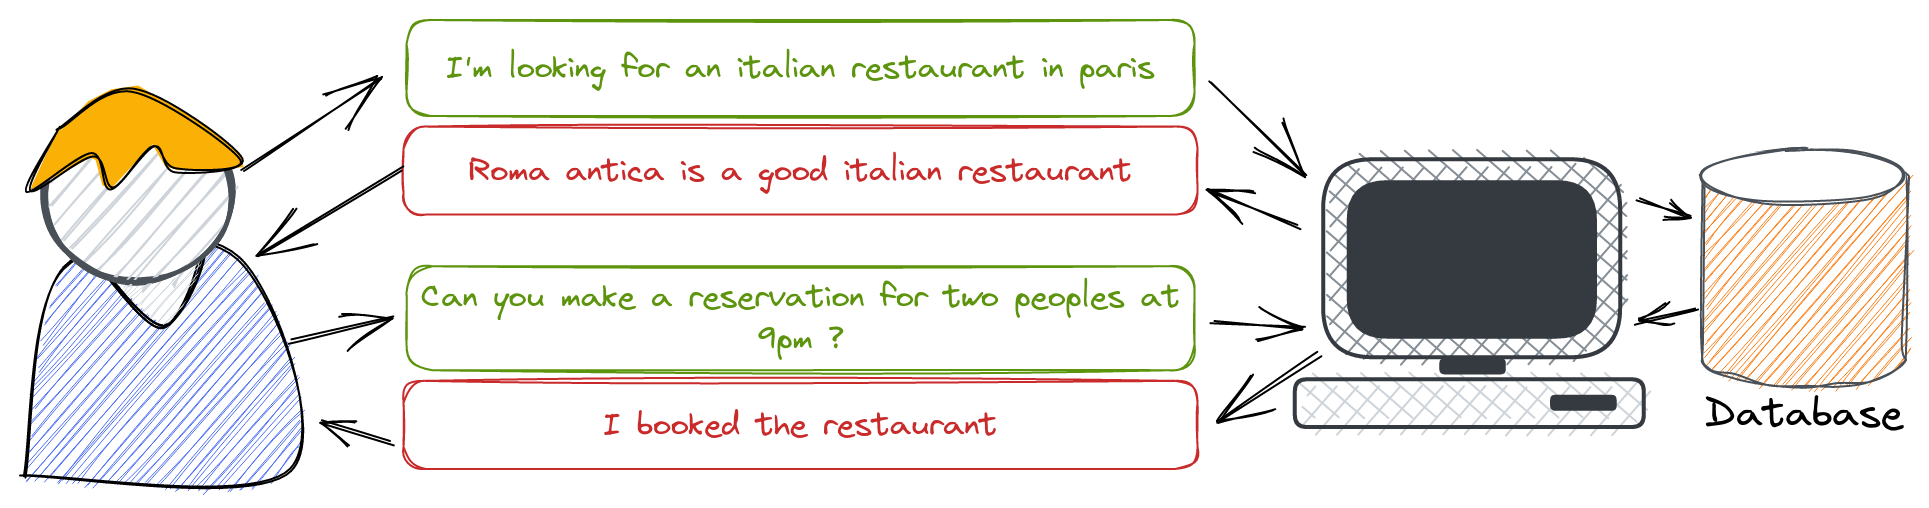
\includegraphics[width=.9\textwidth]{media/task-dial-5.png}
    \end{figure}
    \begin{columns}
        \begin{column}{0.5\textwidth}
            \begin{block}{System Answer}
                \begin{itemize}
                    \item Take into account previous utterances
                \end{itemize}
            \end{block}
        \end{column}

    \end{columns}
\end{frame}
%%% RAZA
\begin{frame}{Tasks Based dialogue systems}
    \begin{columns}
        \begin{column}{0.5\textwidth}
            \begin{block}{System: }
                \begin{itemize}
                    \item Provide a service, obtain specific informations or help user for a task
                    \item Query/update a structured database or a knowledge base
                \end{itemize}
            \end{block}
            \begin{block}{What kind of tasks : }
                \begin{itemize}
                    \item Dialogue based Agenda
                    \item Booking accomodations/restaurants
                    \item Custumer services
                    \item Medical assistant
                \end{itemize}
            \end{block}
        \end{column}
        \begin{column}{0.5\textwidth}
            \begin{block}{WHat we need}
                \begin{itemize}
                    \item Understand what is the user goal (intent)
                    \item Gather multiple turns informations related to user task
                    \item Act (filling a database), inform the user
                    \item Answering in Natural language
                \end{itemize}
            \end{block}
        \end{column}
    \end{columns}
\end{frame}

\begin{frame}{A classical Pipeline}

        \begin{block}{Different Modules :}
            \begin{itemize}
                \item \textbf{NLU}(understanding): \textbf{N}atural \textbf{L}anguage \textbf{U}nderstanding system. It's objective is to interpret user utterances and retrieve, classify or select the different information needed by the system. 
                \item \textbf{DST}(Dialogue Manager): \textbf{D}ialogue \textbf{S}tate \textbf{T}racking. The objective is to keep different information up-to-date (on multiple dialogue turns).
                \item \textbf{Policy}(Dialogue Manager): Selecting what to do, objective is to determine what actions or information the user request. It is often related to the state where the decision is often based upon it. 
                \item \textbf{NLG}: \textbf{N}atural \textbf{L}anguage \textbf{G}eneration aims to generate an answer based on dialogue manager informations, it process the ``system intent'' to make it understandable by user.
            \end{itemize}
        \end{block}
 
\end{frame}

\begin{frame}
    \begin{figure}
        \centering
        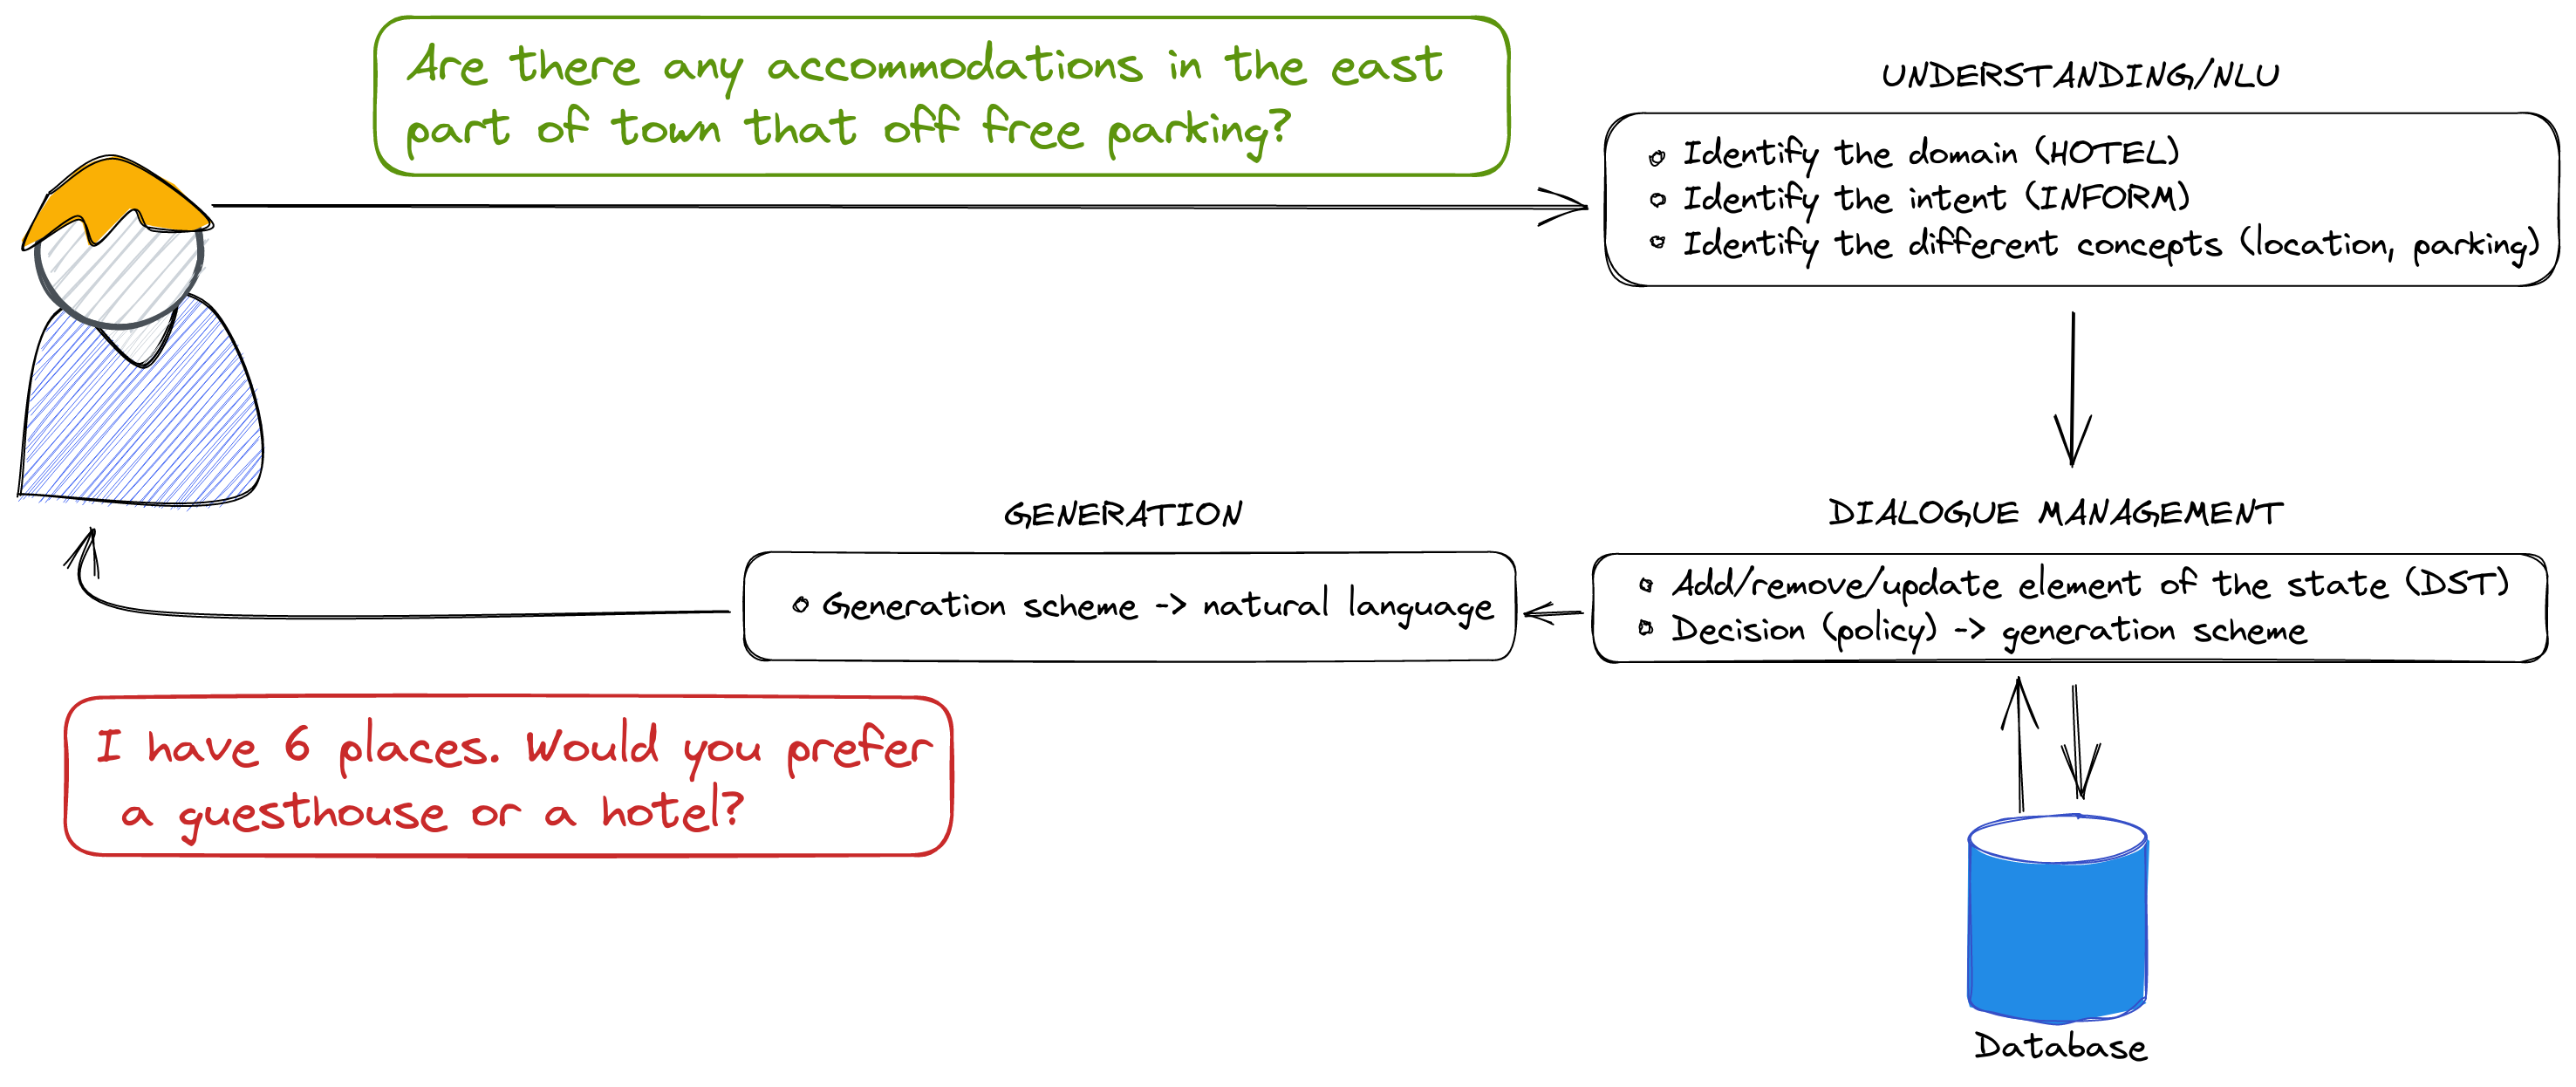
\includegraphics[width=1.\textwidth]{media/dialogue_task_complete.png}
    \end{figure}
\end{frame}

\begin{frame}{An exemple}
\begin{figure}
    \centering
    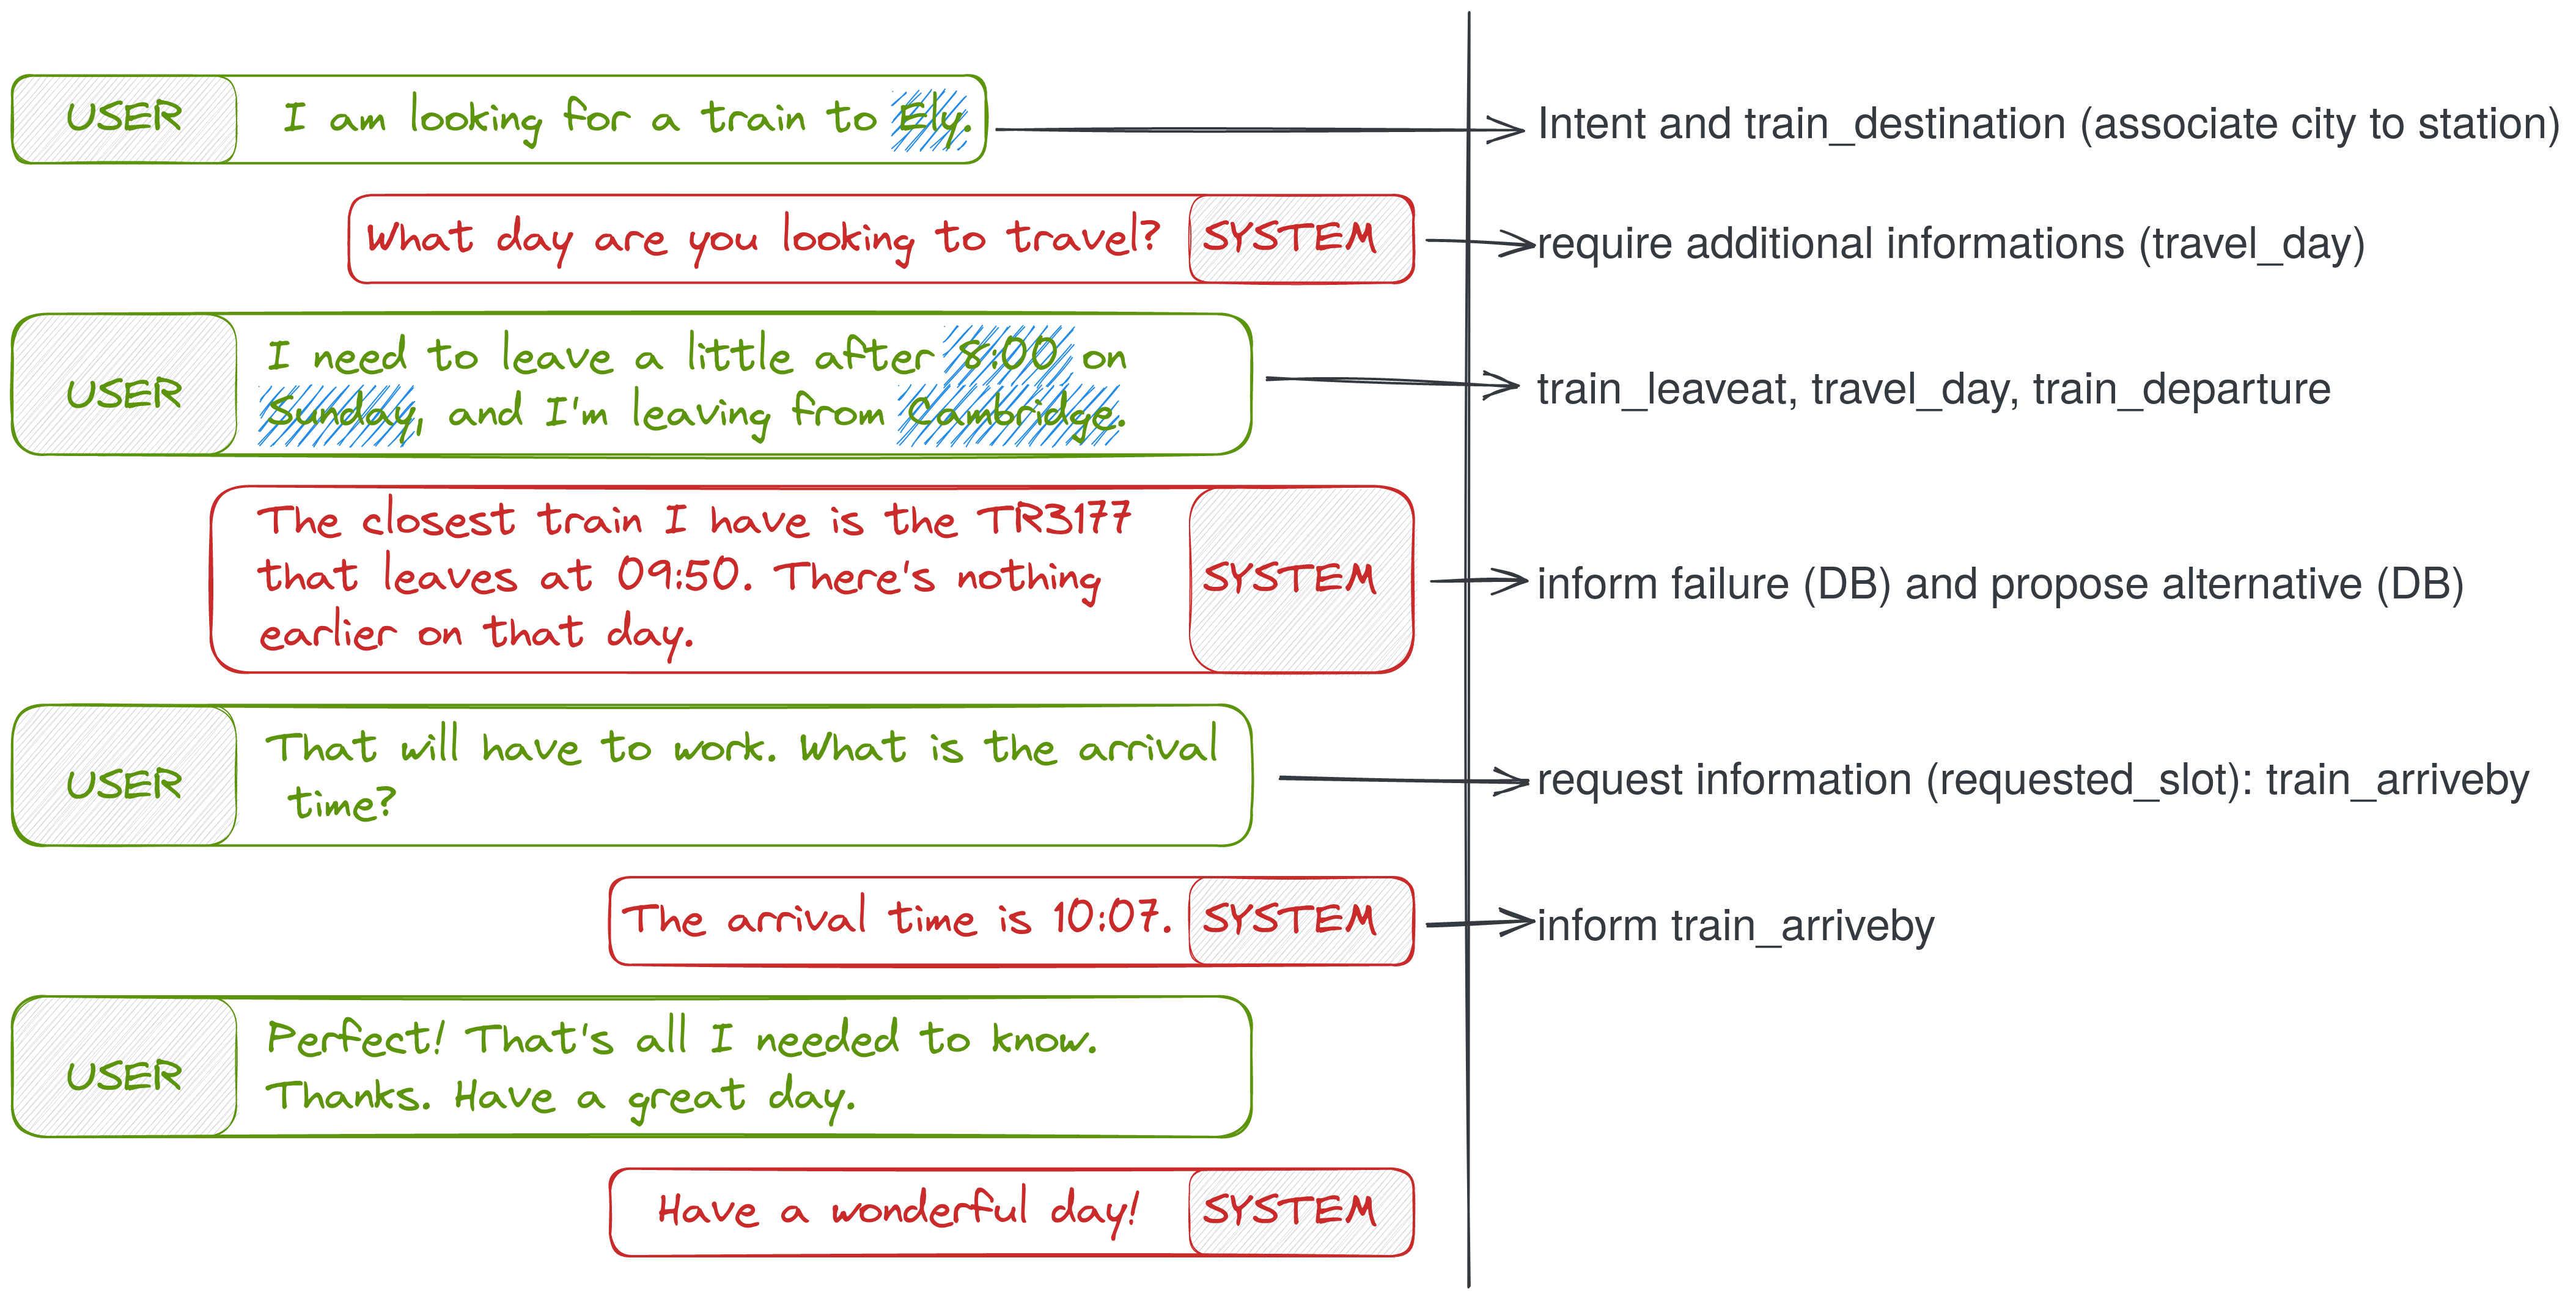
\includegraphics[width=1.\textwidth]{media/dialogue_task_train.png}
    \caption{Example of a dialogue from the MultiWoZ dataset (train booking)}
    \label{fig:example_train_dial_task}
\end{figure}
\end{frame}


\begin{frame}{The NLU task}
    \begin{figure}
        \centering
        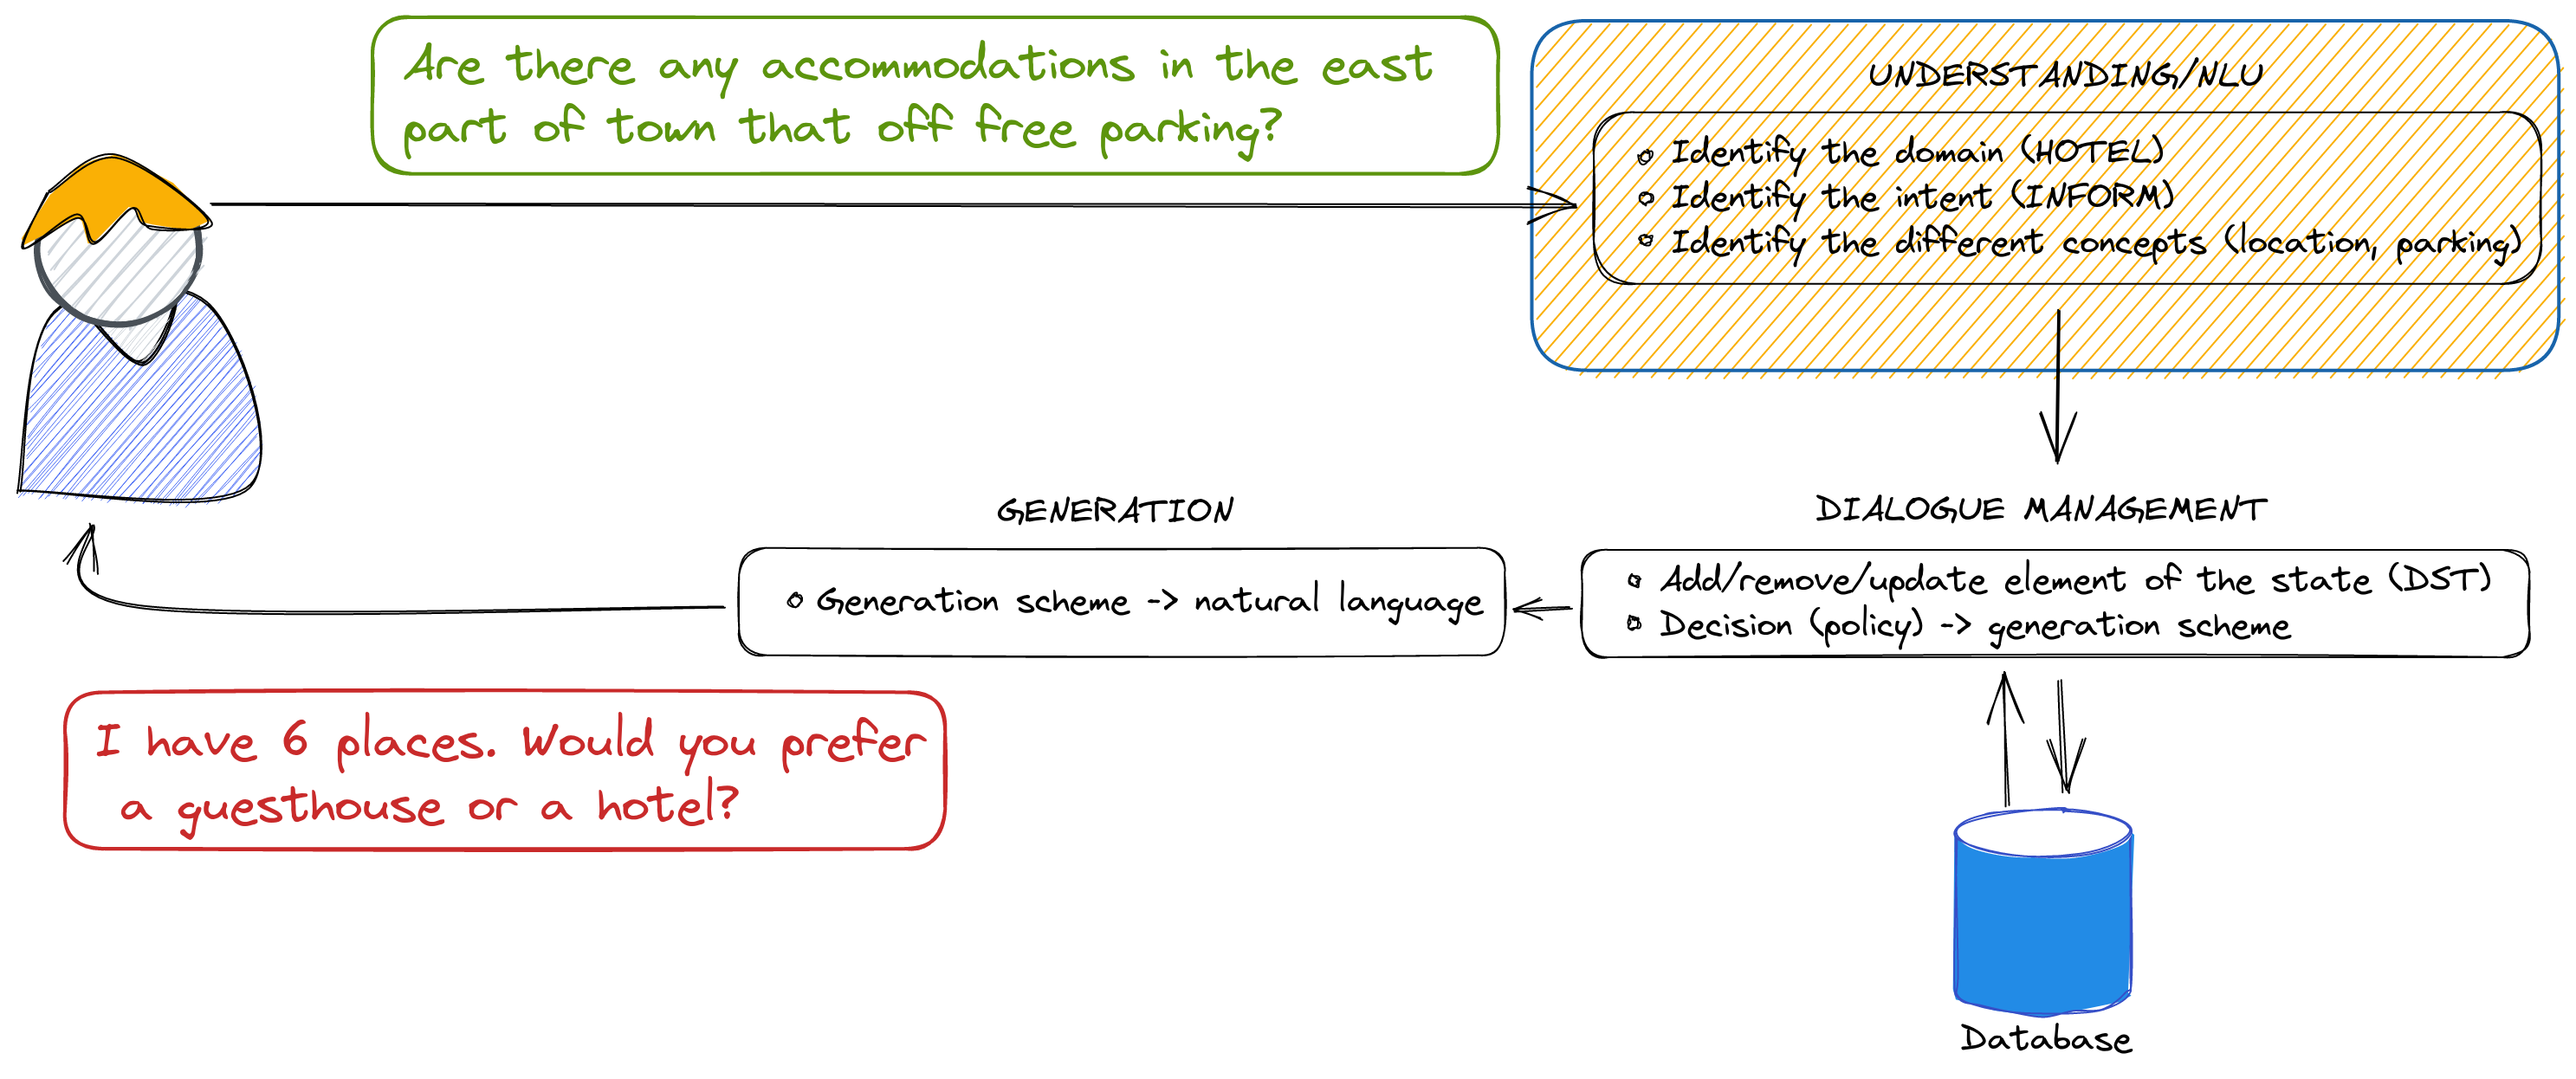
\includegraphics[width=1.\textwidth]{media/dialogue_task_complete_nlu.png}
    \end{figure}
\end{frame}
\begin{frame}{The NLU task : different subtasks}
    \begin{columns}
        \begin{column}{0.5\textwidth}
            \begin{figure}
                \centering
                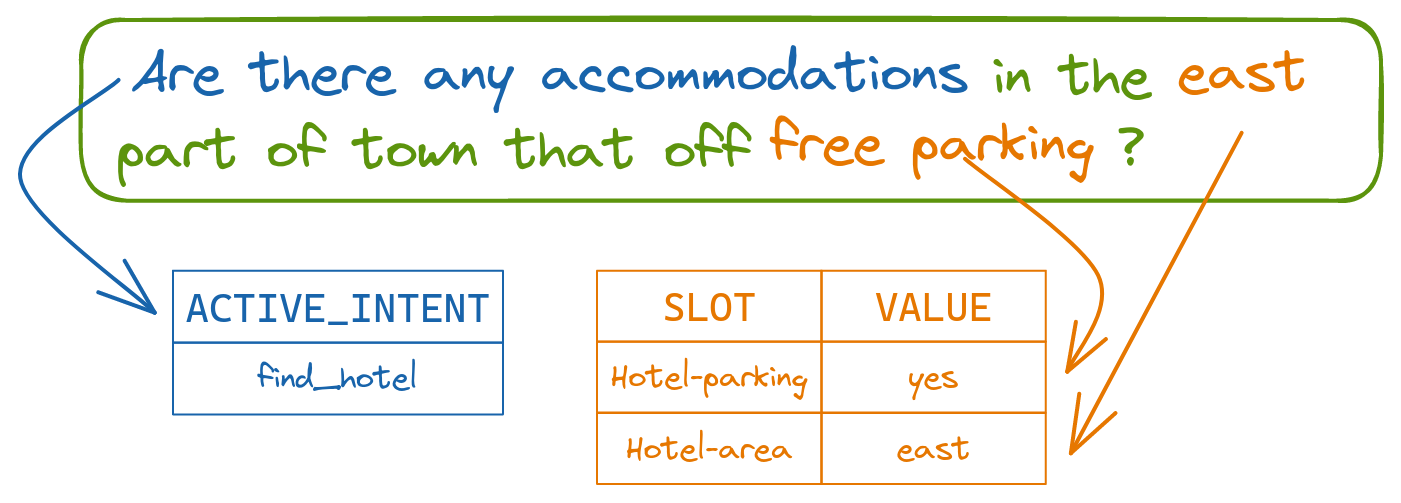
\includegraphics[width=1.\textwidth]{media/attent_slot.png}
            \end{figure}
            \begin{block}{Objective:}
                Retrieve in utterance the relevant information: 
            \begin{itemize}
                \item \textbf{Domain} $\longrightarrow$ HOTEL 
                \item \textbf{Intent} $\longrightarrow$ find\_hotel
                \item \textbf{Concepts:} 
                \begin{itemize}
                    \item hotel-parking $\longrightarrow$ yes
                    \item hotel-area $\longrightarrow$ east
                \end{itemize}
            \end{itemize}
            \end{block}
        \end{column}
        \begin{column}{0.5\textwidth}
            \begin{block}{Often a set of substasks: }
                

            \begin{itemize}
                \item Detection/identification of :
                    \begin{itemize}
                        \item Domain (Multi-domain applications)
                        \item Intention (Always)
                    \end{itemize}
                \item Concept detection:
                    \begin{itemize}
                        \item slot-type (class of the concept, what kind of information)
                        \item slot-value (value of the concept, what value to store)
                    \end{itemize}
            \end{itemize}
            This split appeared in early 2010s \cite{mori-2011-spoken} it is highly related to the development of statistical approaches
            
            \end{block}
        \end{column}
    \end{columns}
\end{frame}

\begin{frame}{The NLU task : Classify the intent}
    \begin{columns}
        \begin{column}{0.5\textwidth}
    \begin{block}{Formalisation}
        Let be $u_i$ and $c_i$ respectivelly the $i^{th}$ utterance and $c_i$ the domain-intent associated to the utterance. We define $D_k$ :
        $$
            D_k = [(u_i, c_i) | \forall i \in \mathbb{N}, i \leq k]
        $$
    \end{block}
    \begin{block}{Domains Identification}
    
        \begin{itemize}
            \item Supervised Learning Classification
            \item The objective is to train a classifier using $u_{k+1}$ and optionally $D_k$.
        \end{itemize}
    \end{block}
    \end{column}
        \begin{column}{0.5\textwidth}
            \begin{block}{What kind of classifiers}
                \begin{itemize}
                    \item SVM (on BOW/TF-IDF/Word embedding), Entity based \ldots
                    \item RNN and LSTM 
                    \item Transformer (BERT like) \cite{wu-2020-tod} ([CLS] classification)
                \end{itemize}
                
            \end{block}
        \end{column}
    \end{columns}
\end{frame}
\begin{frame}{The NLU task: Slots}
    \begin{block}{What is a slot}
        A slot is an information that we would store to better answer, it will additionnaly allow to update the state.\\ \quad \textbf{exemple :}   ``symptom'' (slot name), ``fever'' (slot value)
    \end{block}
    \begin{block}{Slots \& slots value :}
        In most task based dialogue different slots  can be defined. We can consider two types of slots: 
        \begin{itemize}
            \item \textbf{Categorical slots:} The differents possible values for the slot is finite, but are not always explicit in the text \\
            \quad  \textbf{Example } $\rightarrow$ a day in a week (7 values from Monday to Sunday)
            \item \textbf{Extractive slots:} It correspond to an entity or a part that cannot be categorized in the text such as most of named entities \\
            \quad  \textbf{Example 1} $\rightarrow$ a date (not recommended to categorize all posibilities)
            \\
            \quad  \textbf{Example 2} $\rightarrow$ a name of a place (e.g. restaurant, hotel, airport, ...)
        \end{itemize}
    \end{block}

\end{frame}
\begin{frame}{The NLU task: slot, an example}
        \begin{columns}
        \begin{column}{0.6\textwidth}
            \begin{table}[]
                \footnotesize
                \begin{tabular}{l|p{4cm}|c}
                     Slot Name & Description & Categorical\\
                     \largehline
                     train-arriveby & arrival time of the train & \textcolor{red}{FALSE}\\
                     train-leaveat & leaving time for the train & \textcolor{red}{FALSE} \\
                      train-duration & duration of the travel & \textcolor{red}{FALSE} \\
                     train-departure & departure location of the train & \textcolor{green}{TRUE} \\
                     train-destination & destination of the train & \textcolor{green}{TRUE} \\
                     train-day &  day of the train & \textcolor{green}{TRUE} \\
                     train-bookpeople & how many train tickets you need & \textcolor{green}{TRUE} \\
                     train-price & price of the train & \textcolor{red}{FALSE} \\
                     train-ref & reference number of the train booking & \textcolor{red}{FALSE}\\
                     train-trainid & id of the train & \textcolor{red}{FALSE} \\
                     

                     
                \end{tabular}
                \caption{The different slots for the ``train'' domain in MultiWoZ}
                \label{table:example_slot_train}
            \end{table}
        \end{column}
        \begin{column}{0.4\textwidth}
            \begin{block}{In the NLU System :}
                \begin{itemize}
                    \item Extract part of the utterance reffering to categorical slots
                    \item Classify utterances or text extracted to retrieve the different categorical pair slots values (e.g. mapping extracted value to closest value in the dataset)
                \end{itemize}
                
            \end{block}

        \end{column}
    \end{columns}
\end{frame}
\begin{frame}{The NLU task: slots, scheme example}
    \begin{figure}
        \centering
        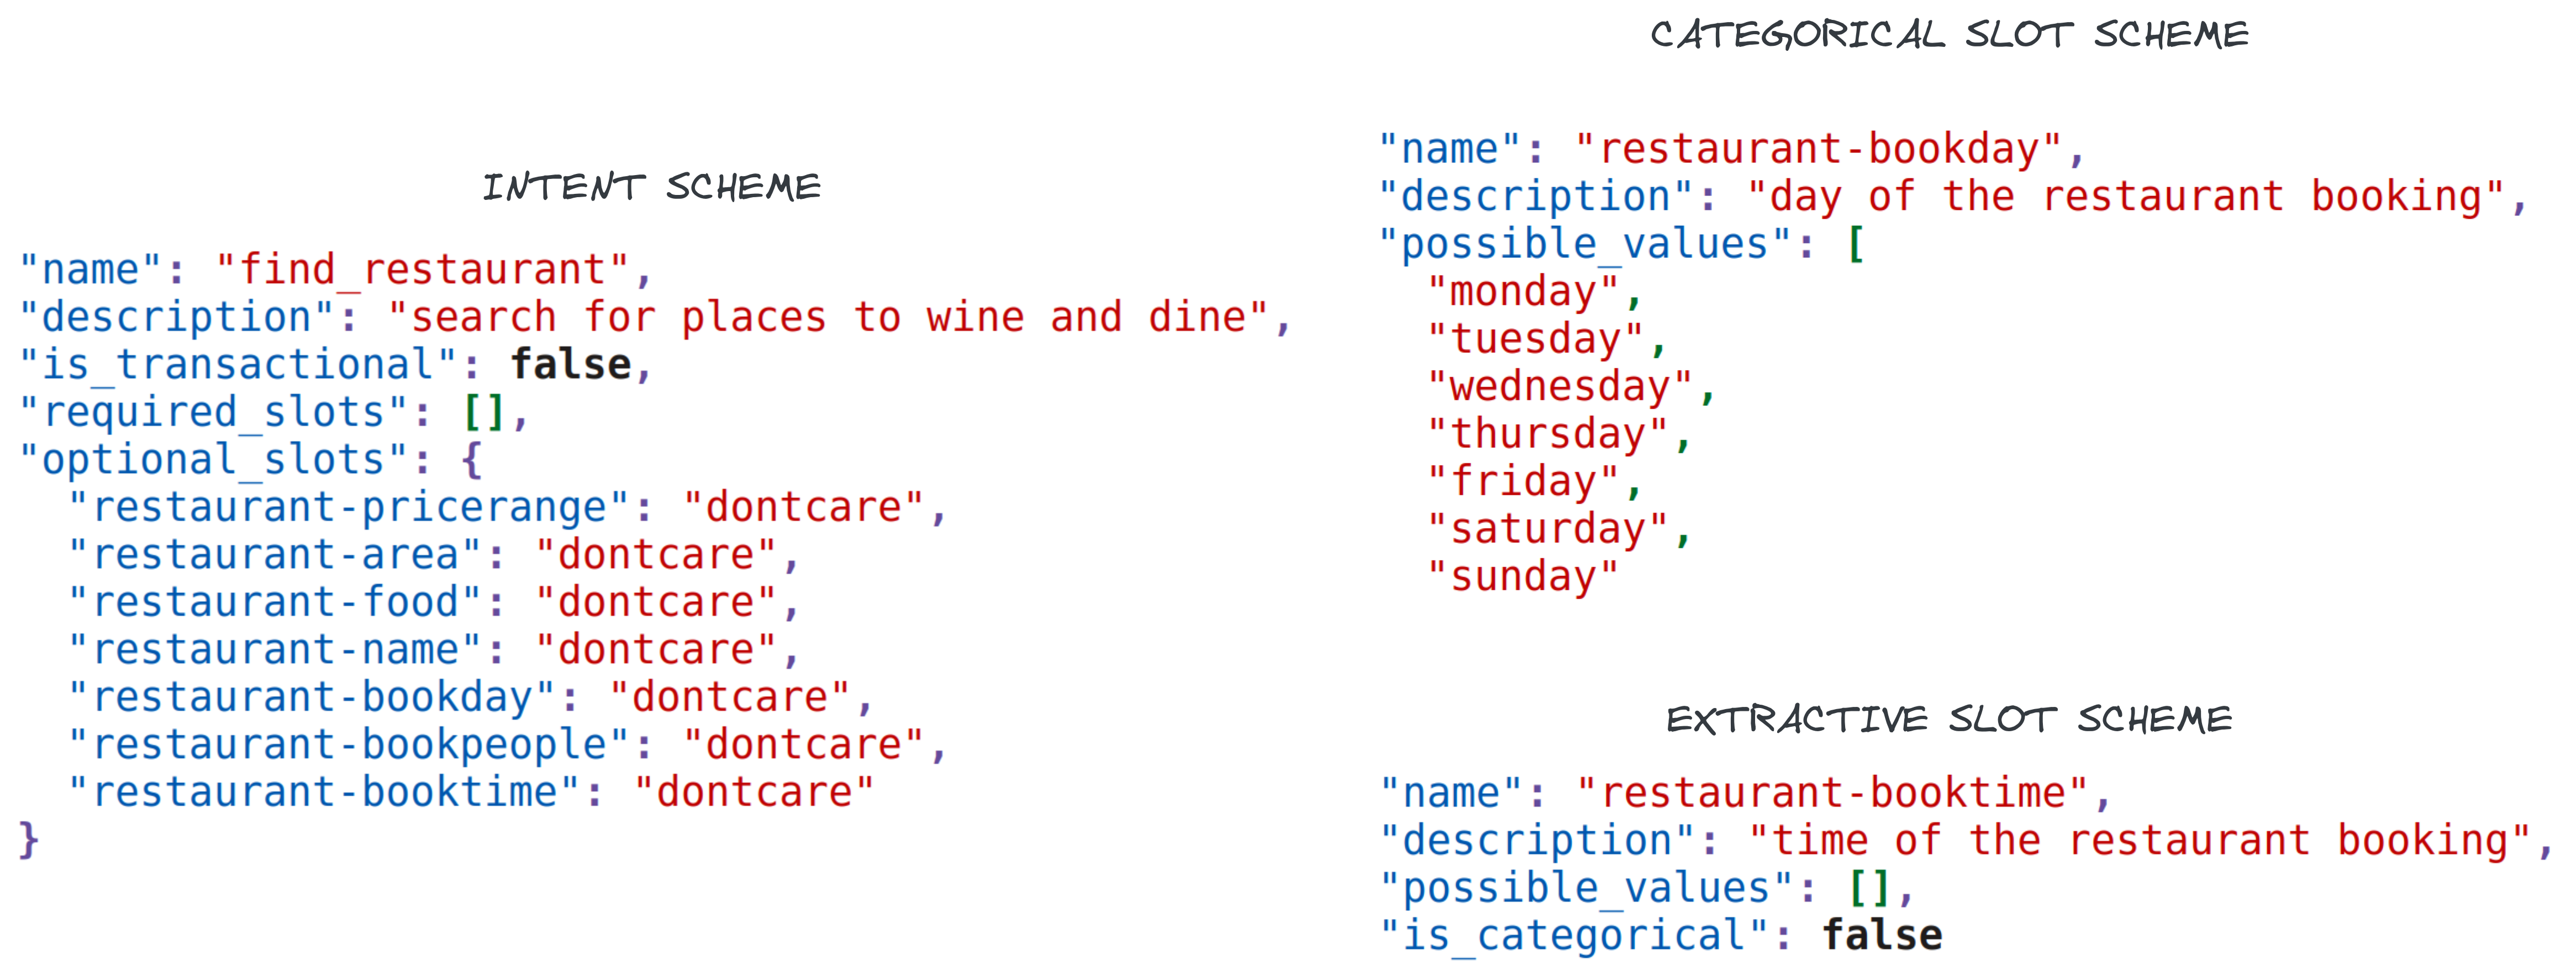
\includegraphics[width=1.\textwidth]{media/example_scheme.png}
        \caption{An example of a scheme in MultiWoZ (restaurant domain)}
        \label{fig:my_label}
    \end{figure}
\end{frame}

\begin{frame}{The NLU task: Slot filling (CRF)}

% + Generative and Discriminative Algorithms for Spoken Language
% Understanding
% Christian Raymond, Giuseppe Riccard
    \begin{figure}
        \centering
        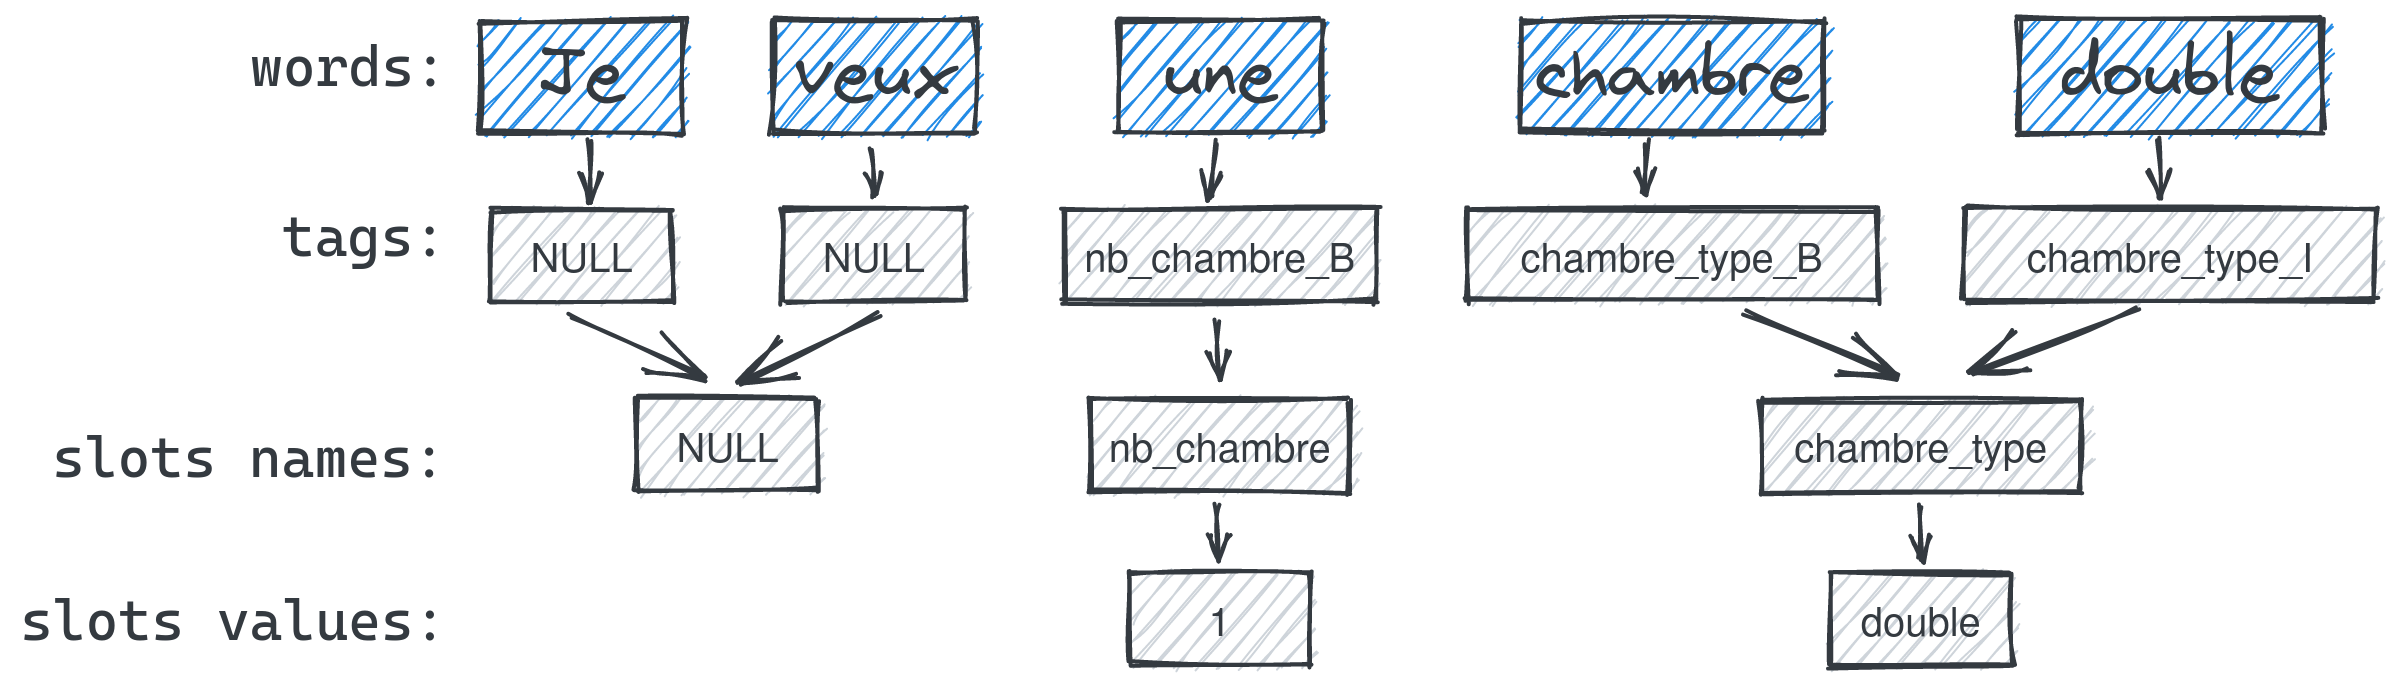
\includegraphics[width=.75\textwidth]{media/hahn_figure_crf.png}
        \label{fig:hahn-split}
    \end{figure}
    \begin{block}{Conditional Random Field framework \cite{hahn-2011-comparing}:}
        Different tags for each slots (see figure below). The objective is to estimate the probability of tags sequence $t_1^N =  \{t_i| i \leq N, i \in \mathbb{N} \}$ according to word sequence $w_1^N = \{w_i| i \leq N, i \in \mathbb{N} \}$ i.e. estimate the posterior (CRF) $p(t_1^N|w_1^N) = Z^{-1} \prod_{i=1}\limits^N e^{v^th(t_{n-1}, t_{n}, w_1^N)}$, with $h$ the features extraction function (features are based on coocurences of words or tags in the training set). The generation is done by the forward-backward algorithm (close to viterbi algorithm in HMM).
    \end{block}
\end{frame}

\begin{frame}{The NLU task: Slot filling (RNN/LSTM)}
    \begin{figure}
        \centering
        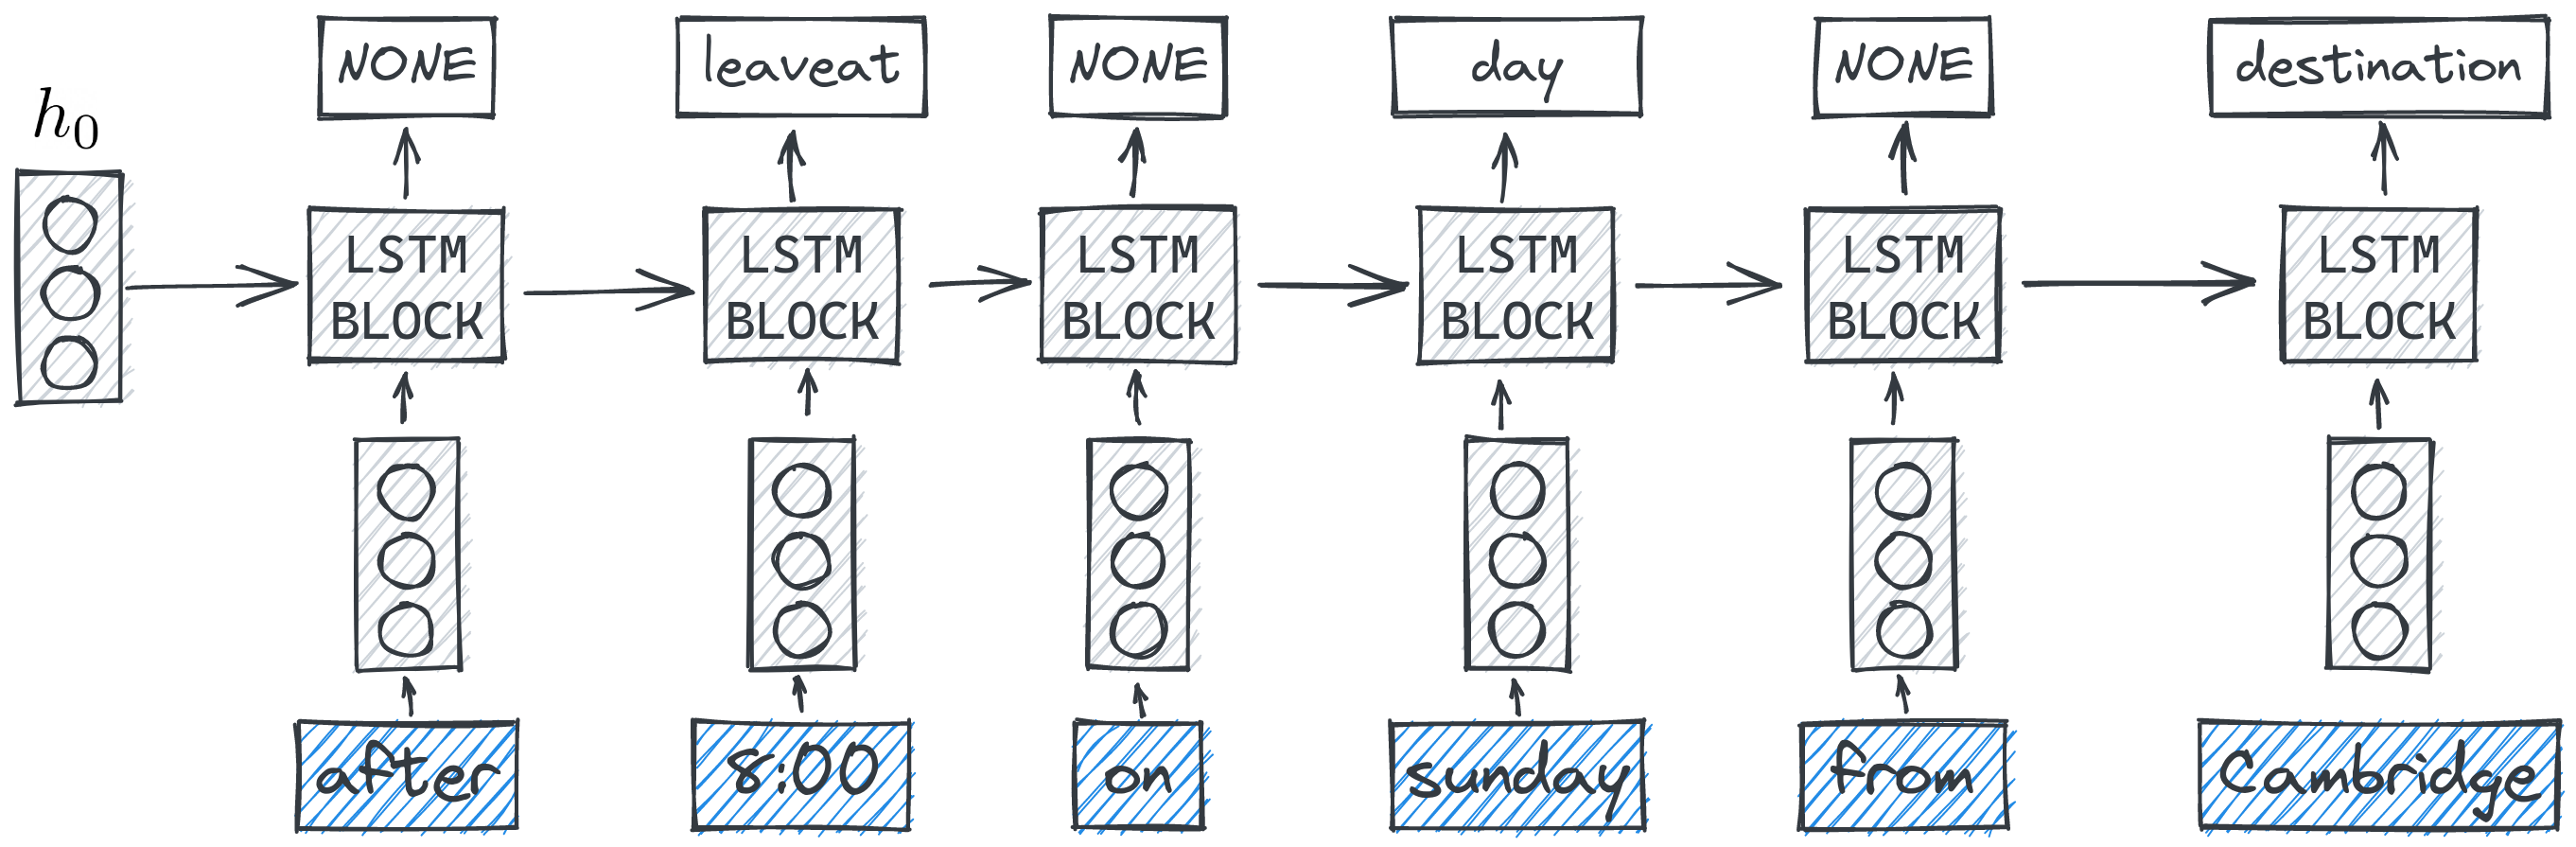
\includegraphics[width=.8\textwidth]{media/rnn_figure_general.png}
        \label{fig:hahn-split}
    \end{figure}

    \begin{block}{RNN:}
        \begin{itemize}
            \item LSTM  with moving average (and deep LSTM with stacked LSTM) \cite{yao-2014-spoken}
            \item Reccurent CRF \cite{mesnil-2015-using} (+learning features)
            \item Bi-LSTM \cite{ghannay-etal-2020-neural} (comparison of different word embeddings)
        \end{itemize}
    \end{block}
\end{frame}

\begin{frame}{The NLU task: Slot filling (Transformer)}

       \begin{columns}
        \begin{column}{0.6\textwidth}
            \begin{figure}
                \centering
                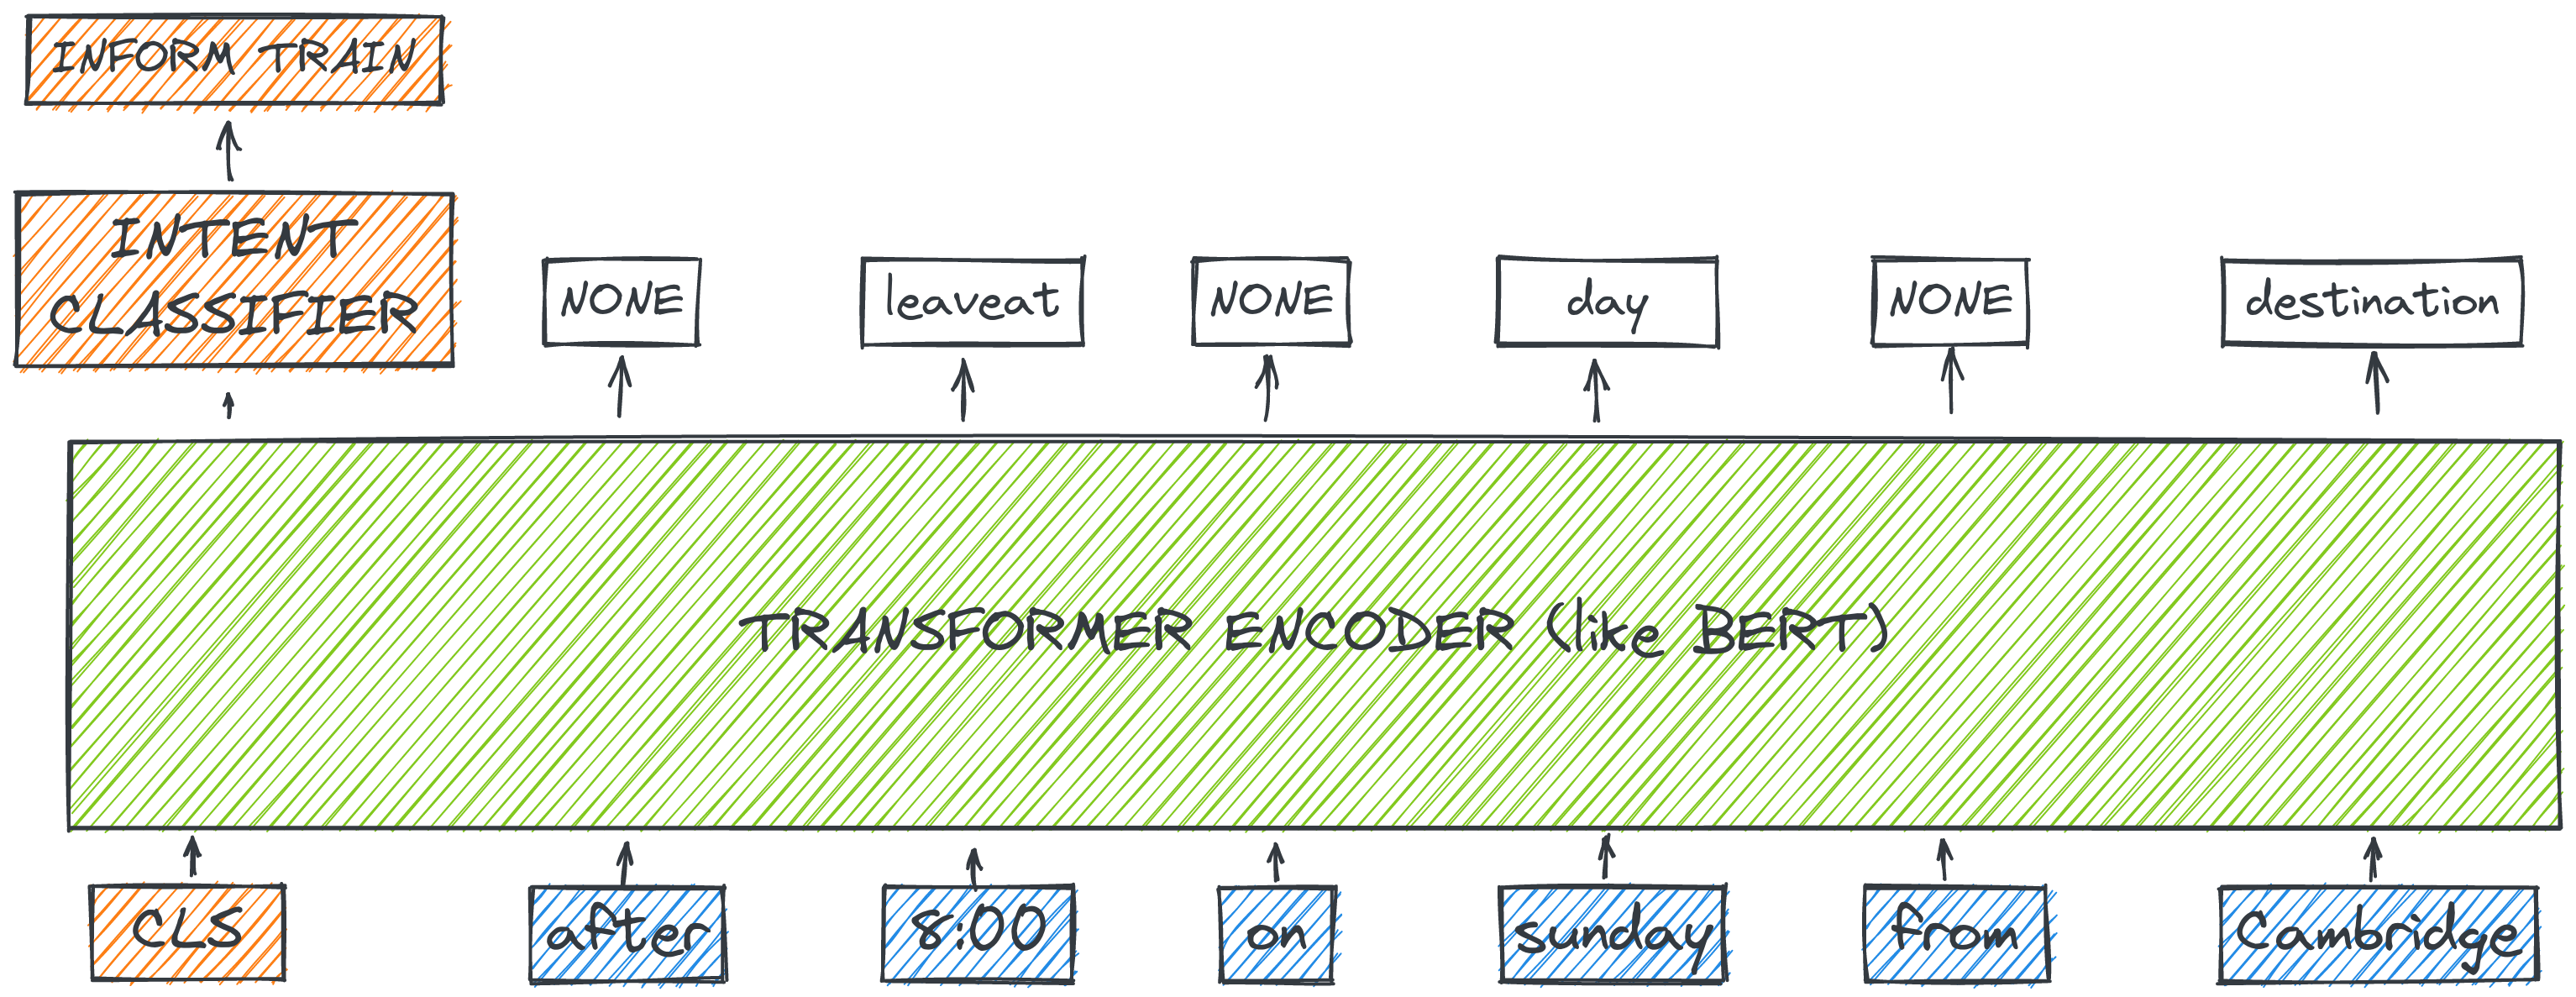
\includegraphics[width=1.\textwidth]{media/transformer-bert-intent-slot.png}
                \label{fig:hahn-split}
            \end{figure}
            \begin{block}{Transformer approaches}
                \begin{itemize}
                    \item Joint Slot Filling and Intent Classification \cite{wu-2020-slotrefine}
                    %BERT for Joint Intent Classification and Slot Filling
                    \item Comparison on the French Corpus Fine-Tunning a CammenBERT model \cite{ghannay-etal-2020-neural} 
                \end{itemize}
                
            \end{block}
        \end{column}
        \begin{column}{0.4\textwidth}
            \begin{figure}
                \centering
                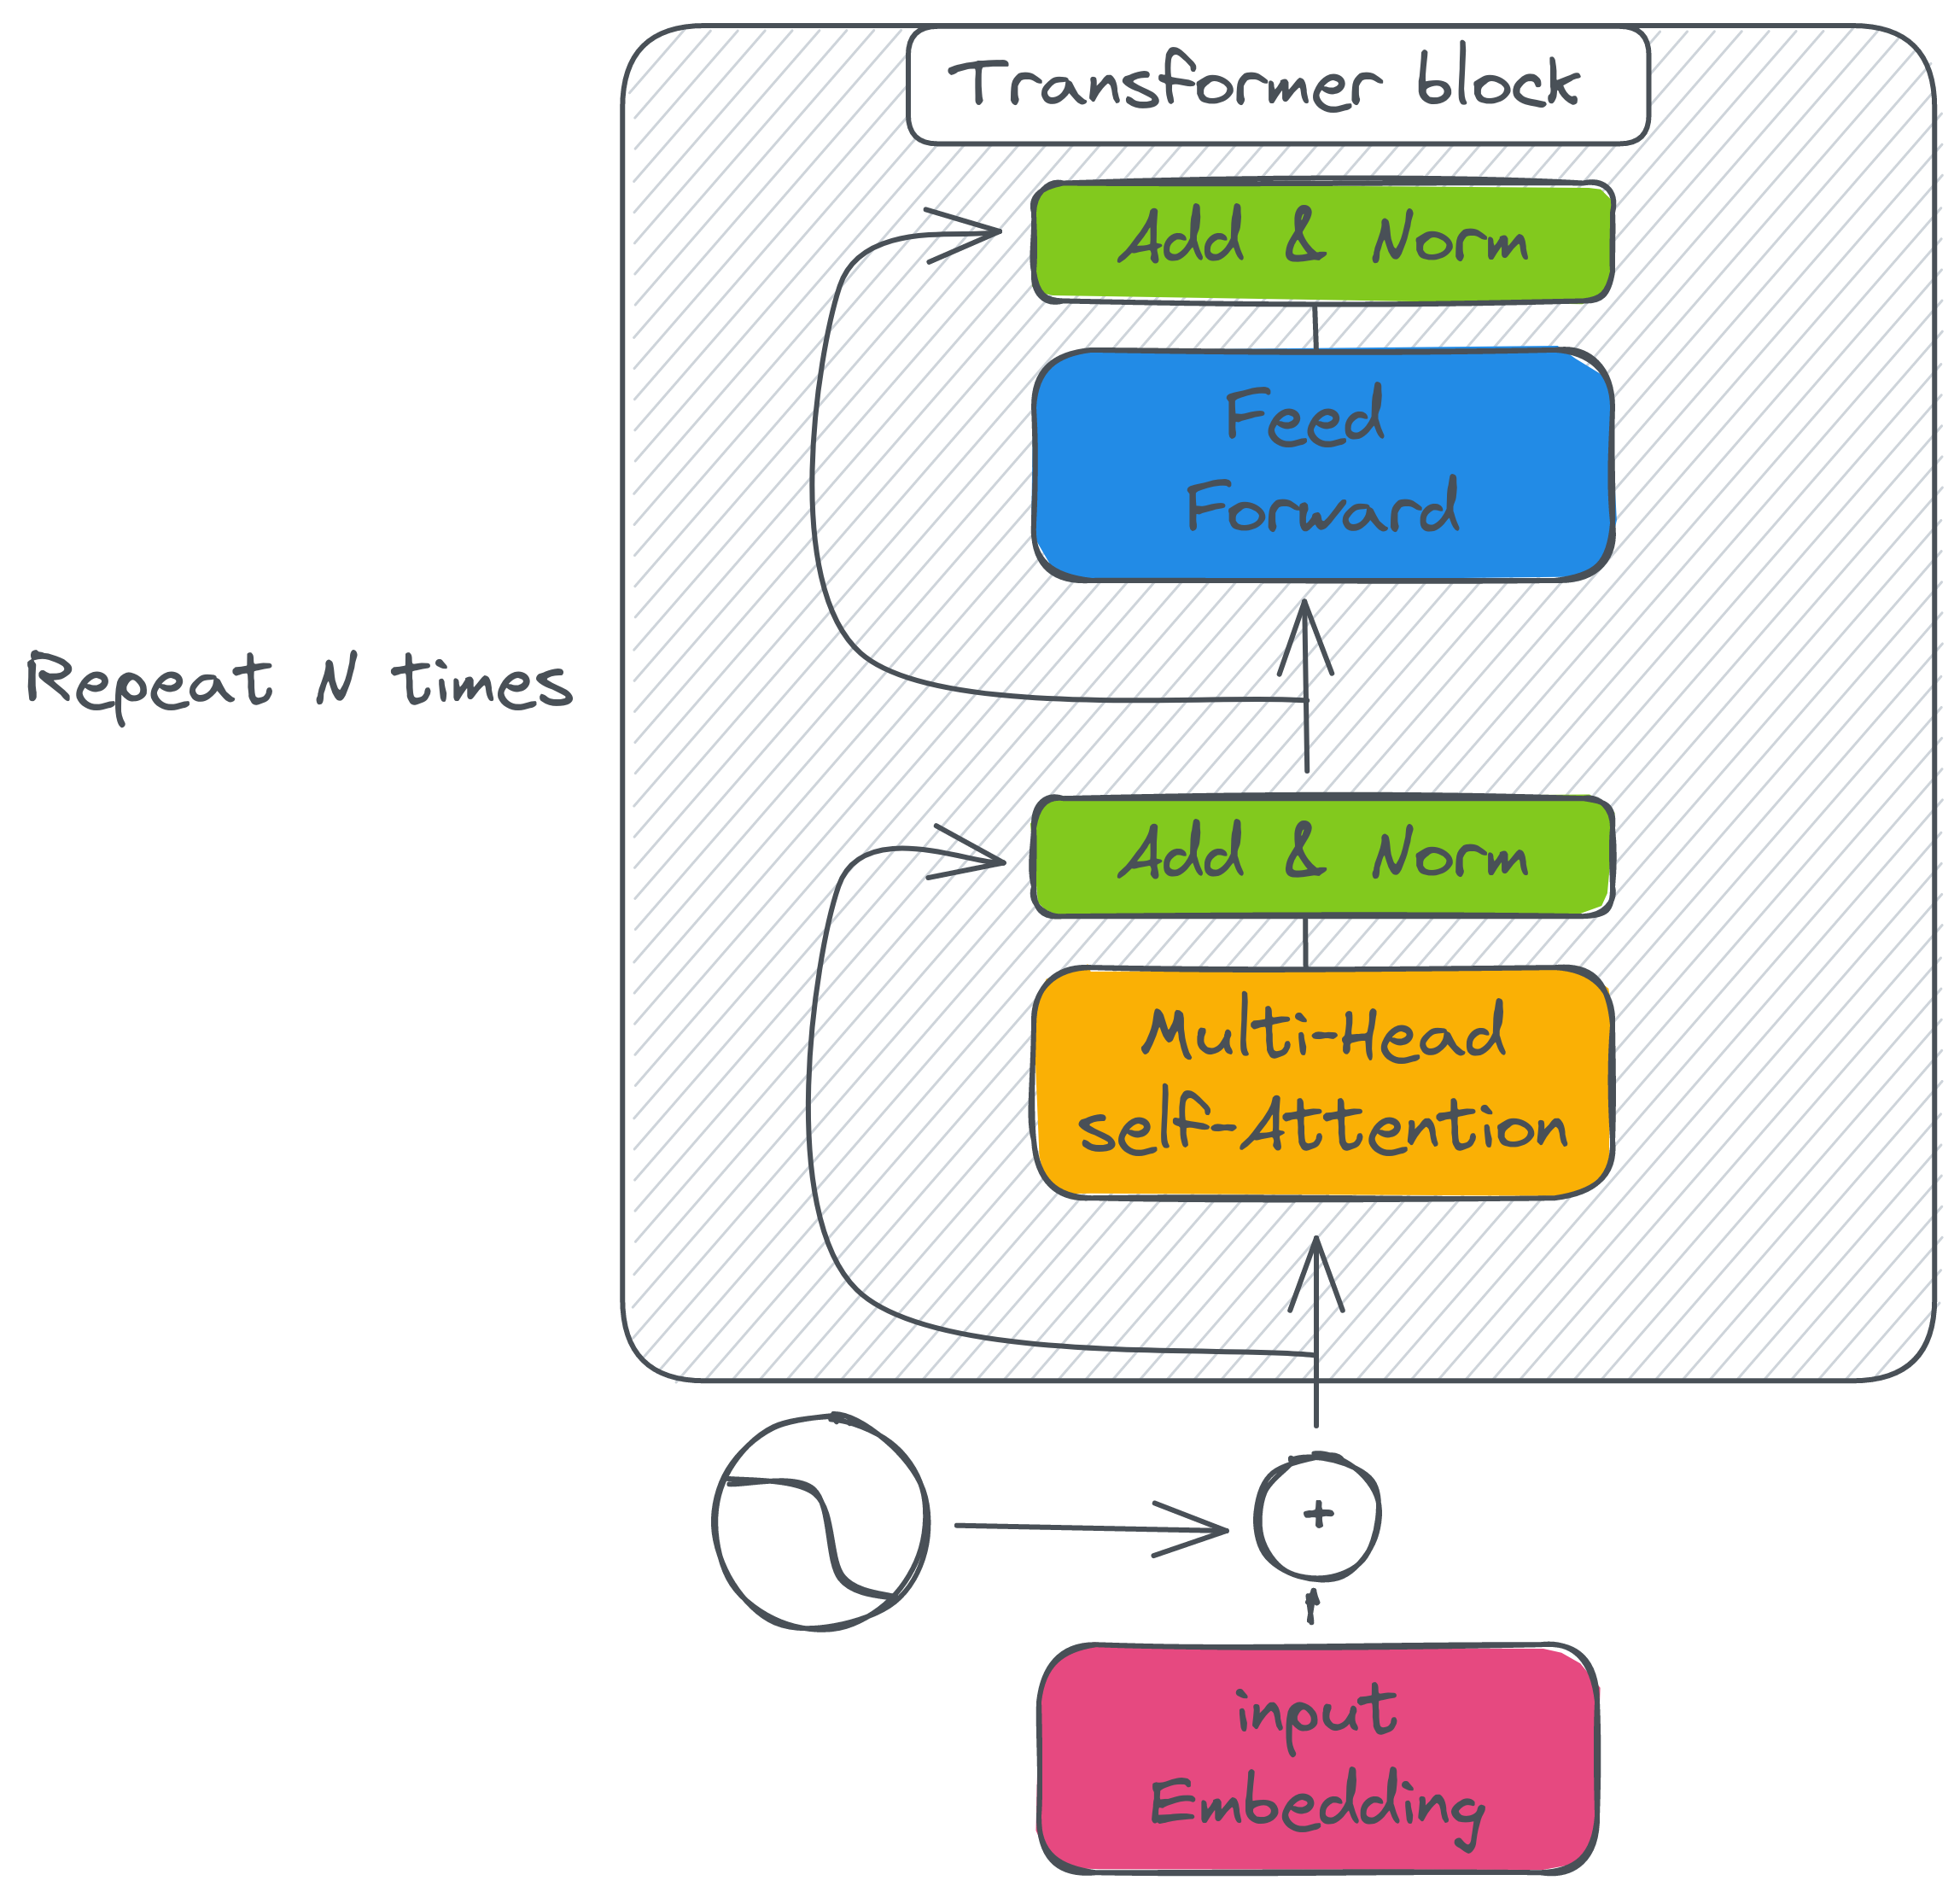
\includegraphics[width=.9\textwidth]{media/transformer-block.png}
                \caption{Transformer block architecture}
            \end{figure}
        \end{column}
    \end{columns}
\end{frame}

\begin{frame}{The NLU task: Slot filling overall information}
    \begin{block}{Other approaches}
        Other kind of approaches exists but are  more rare today (today mainly based on transformers models)
        \begin{itemize}
            \item Logic formula and $\lambda$ calculus \cite{antoine-2004-categorial}
            \item Regular expression \cite{llanos-etal-2016-managing}
            \item Context free grammar \cite{GLASS19951}
        \end{itemize}
    \end{block}

    \begin{block}{Joint Slot filling and Intent classification}
        Learning both in the mean time tends to improve performances (notice that some models previously cited are joint models)
    \end{block}

\end{frame}
\begin{frame}{The NLU task: SLU From audio (ASR/SLU)}
\begin{columns}
    \begin{column}{0.4\textwidth}
        \begin{figure}
            \centering
            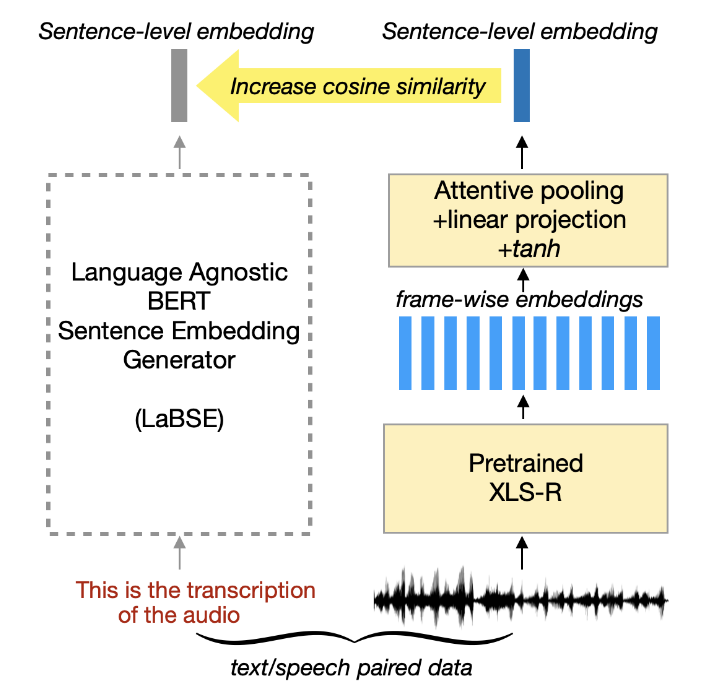
\includegraphics[width=1.\textwidth]{media/slu.png}
            \caption{Architecture of SAMU-XLSR \cite{Khurana_2022_samu}}
            \label{fig:samu}
        \end{figure}
    \end{column}
    \begin{column}{0.6\textwidth}
            \begin{block}{ASR \& SLU}
        An other approach consists in retrieving slot values directly from audio. 
        \begin{itemize}
            \item \textbf{A}utomatic \textbf{S}peech \textbf{R}ecognition transform audio to texte
            \item \textbf{S}poken \textbf{L}anguage \textbf{U}nderstanding interpret the Language
        \end{itemize}
    \end{block}
    \begin{block}{Approaches:}
        \begin{itemize}
            \item SAMU-XLSR \cite{Khurana_2022_samu} (training ASR for semantic analysis)
            \item Few-shot/zero-shot SLU \cite{laperriere-2022-semantically} %ON THE USE OF SEMANTICALLY-ALIGNED SPEECH REPRESENTATIONS FOR SPOKEN LANGUAGE UNDERSTANDING
        \end{itemize}
    \end{block}
    \end{column}
\end{columns}
\end{frame}

\begin{frame}{NLU}
       \begin{columns}
        \begin{column}{0.6\textwidth}
            \begin{block}{What we use today}
                \begin{itemize}
                    \item Mostly transformer classification approaches
                    \item Some consider generative approaches (often DST models in the mean time)
                \end{itemize}
            \end{block}
            \begin{block}{Direction}
                \begin{itemize}
                    \item Transfer for new languages and languages with low ressources \cite{cattan-etal-2021-cross} (multilingual corpus)
                    \item Lifelong learning, learning new terms, concepts during the dialogue \cite{verron-2021-evaluate}
                \end{itemize}
            \end{block}
        \end{column}
        \begin{column}{0.4\textwidth}
            \begin{alertblock}{NLU and DST:}
                Today most of the approaches does not only base on an NLU (Intent + Slot) approach, but also consider in the meantime the DST task !!!
                \begin{itemize}
                    \item A simple review on slot filling and intent classification (mainly datasets) \cite{larson-2022-survey}
                \end{itemize}
            \end{alertblock}

        \end{column}
    \end{columns}
\end{frame}
\section{Dialogue Management}
\begin{frame}{Dialogue Management}
    \begin{figure}
        \centering
        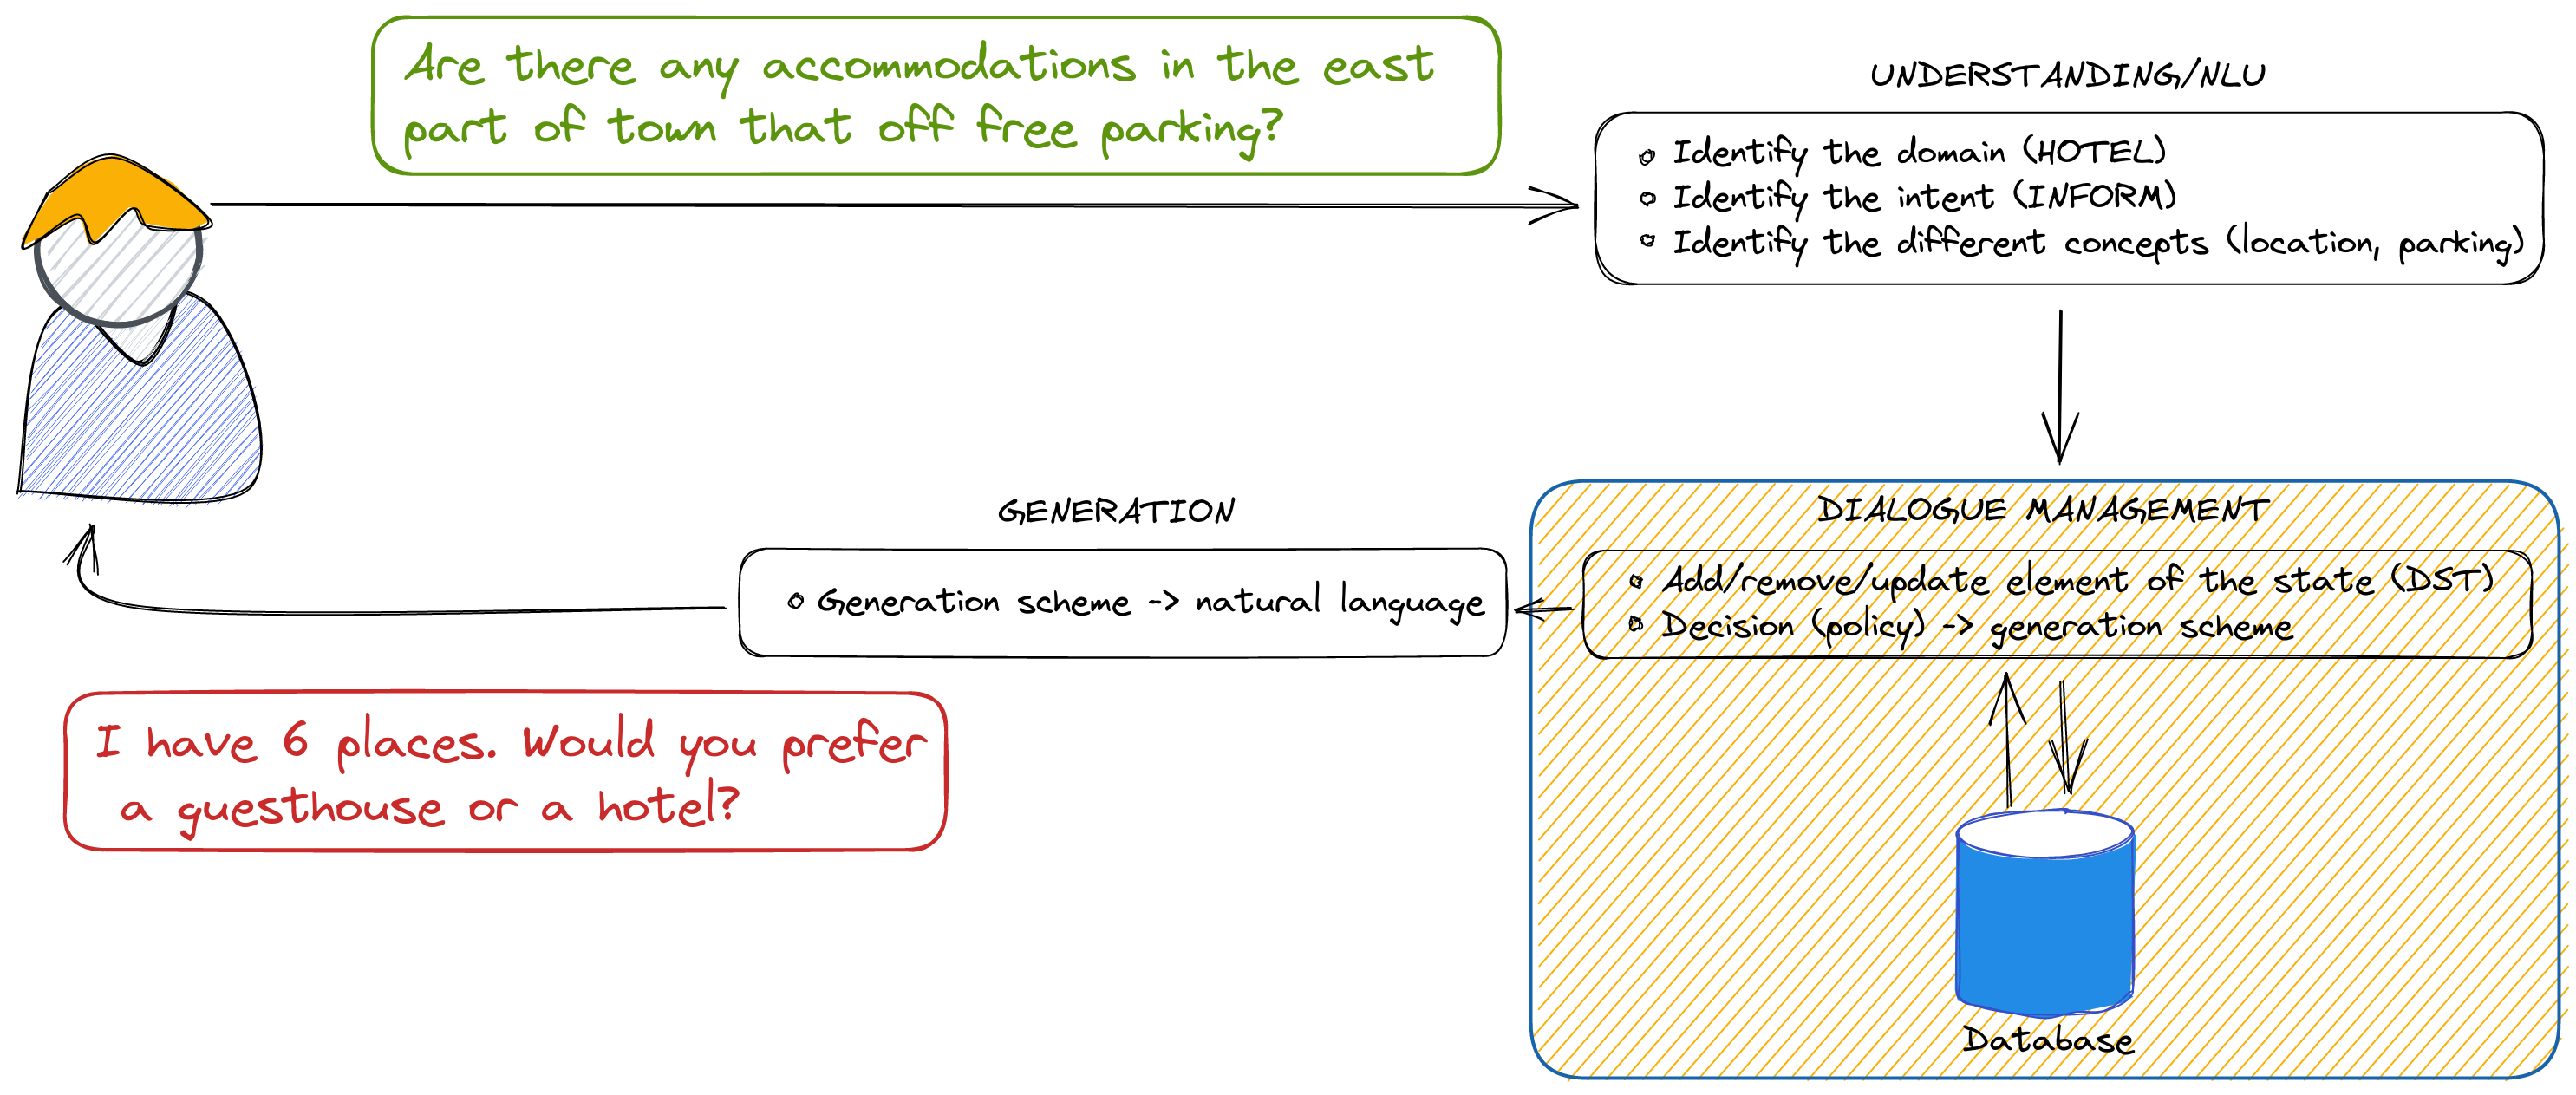
\includegraphics[width=1.\textwidth]{media/dialogue_task_complete_dm.png}
    \end{figure}
\end{frame}
\begin{frame}{Dialogue Management: in context}
    \begin{block}{Understanding in context : multi-turn information}
        Intent user information rarely depends only on one utterance
        \begin{itemize}
            \item Gathering Information all along the dialog
            \item Eventually change and update this informations (slot type/value)
        \end{itemize}
    \end{block}
    \begin{figure}[b]
        \centering
        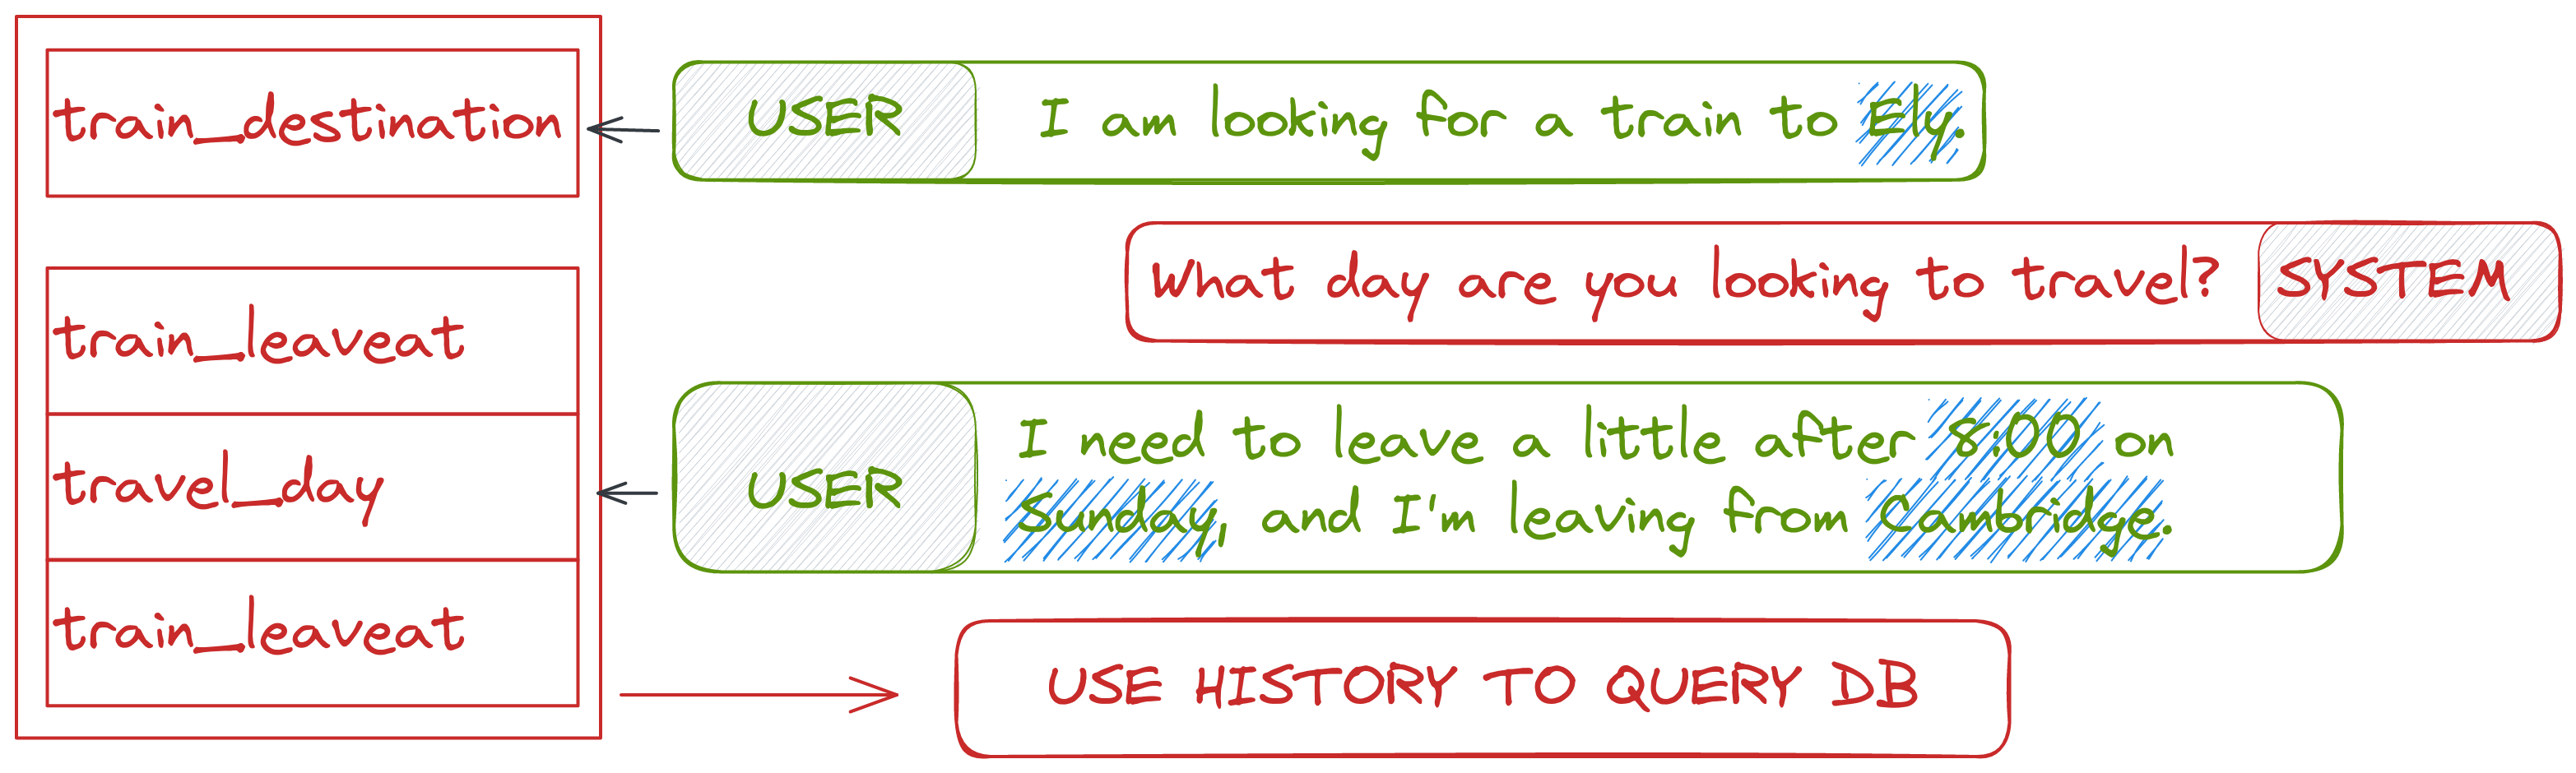
\includegraphics[width=.8\textwidth]{media/in_context_history.png}
        \caption{Gathering information for many utterances}
        \label{fig:my_label}
    \end{figure}
    
\end{frame}

\begin{frame}
    \begin{block}{Understanding in context}
        Utterance make reference to previous one
        \begin{itemize}
            \item Some request are reffering to a previous utterance
            \item Finding what it reffered to (here arrival\_time)
        \end{itemize}
    \end{block}
    \begin{figure}[b]
        \centering
        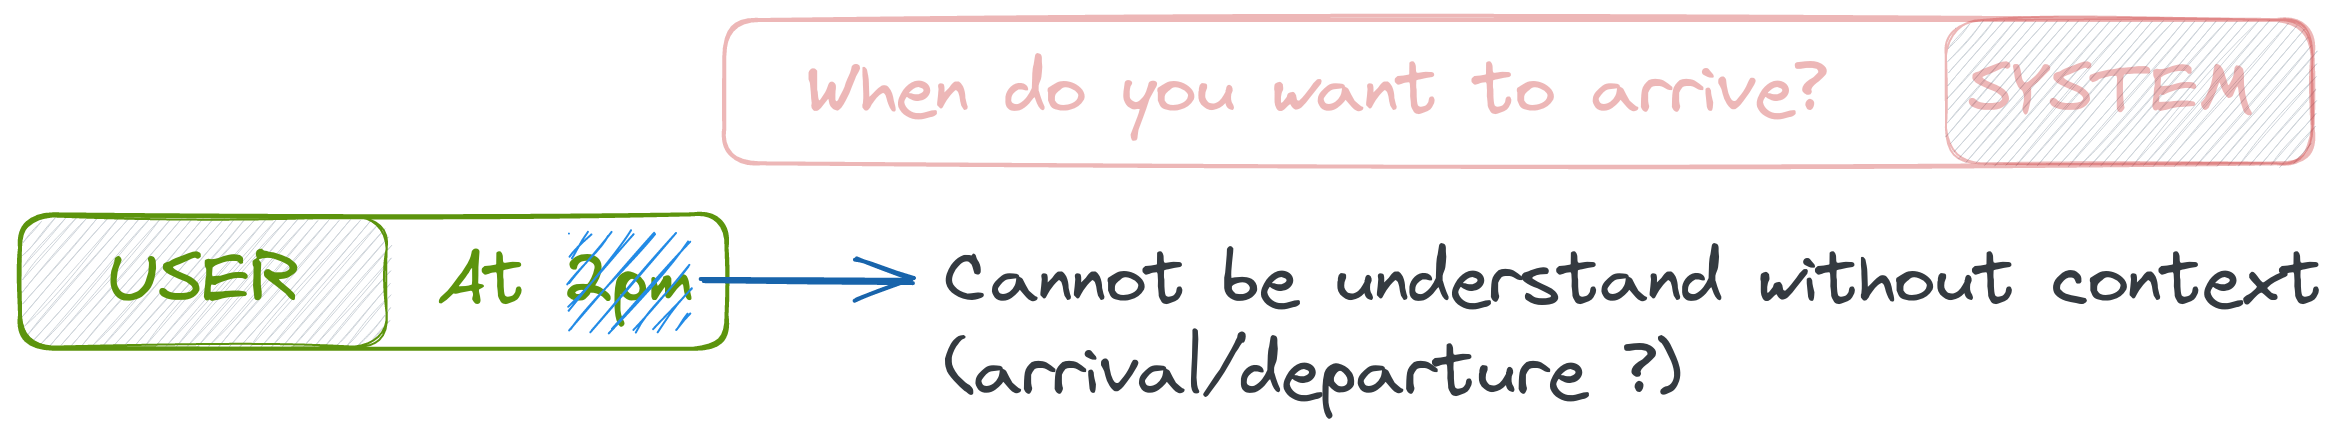
\includegraphics[width=.9\textwidth]{media/in_context_when_0.png}
        \label{fig:my_label}
    \end{figure}
\end{frame}
\begin{frame}[noframenumbering]
    \begin{block}{Understanding in context}
        Utterance make reference to previous one
        \begin{itemize}
            \item Some request are reffering to a previous utterance
            \item Finding what it reffered to (here arrival\_time)
        \end{itemize}
    \end{block}
    \begin{figure}[b]
        \centering
        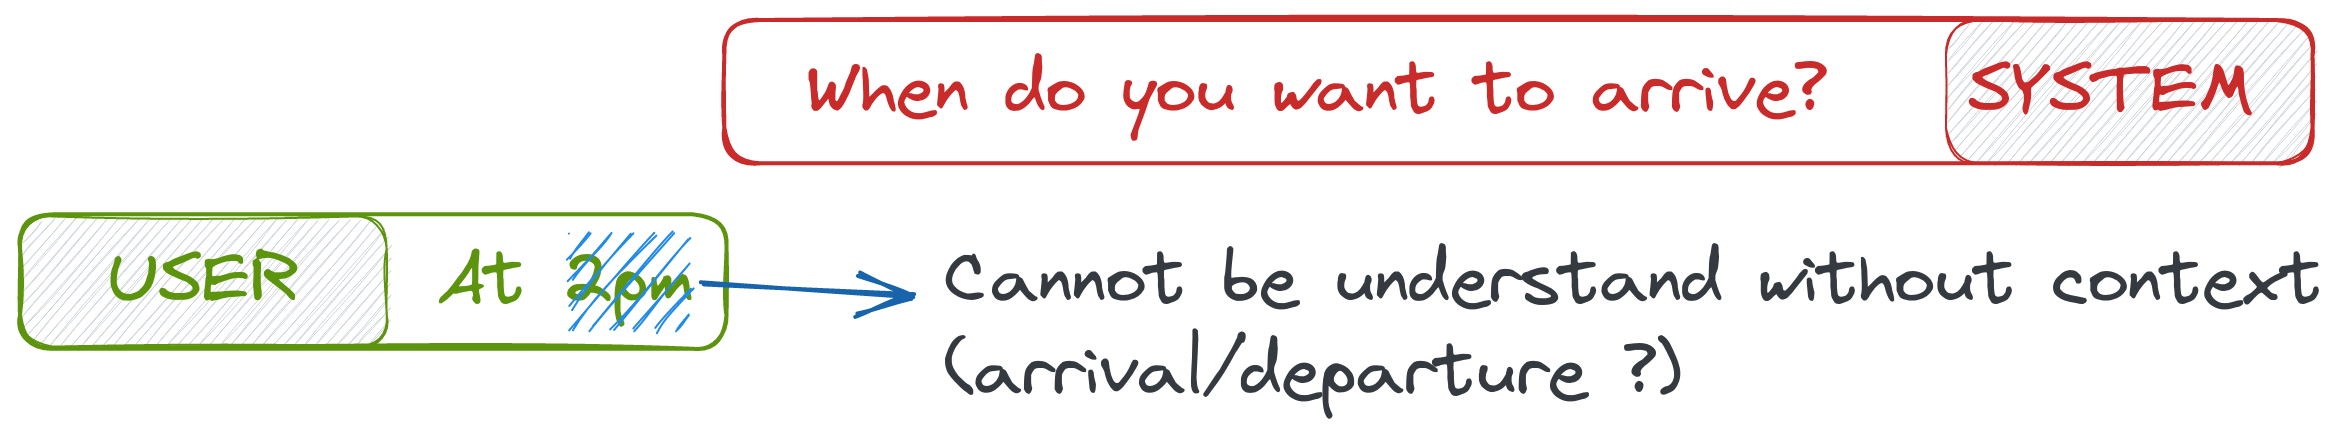
\includegraphics[width=.9\textwidth]{media/in_context_when.png}
        \label{fig:my_label}
    \end{figure}
    
\end{frame}
\begin{frame}
    \begin{block}{Transform slot values (entity linking)}
        \begin{itemize}
            \item Different values extracted reffering to same entities
            \item Information expressed contextually, need to transform to use it (date, time...)
        \end{itemize}
    \end{block}
    \begin{figure}[b]
        \centering
        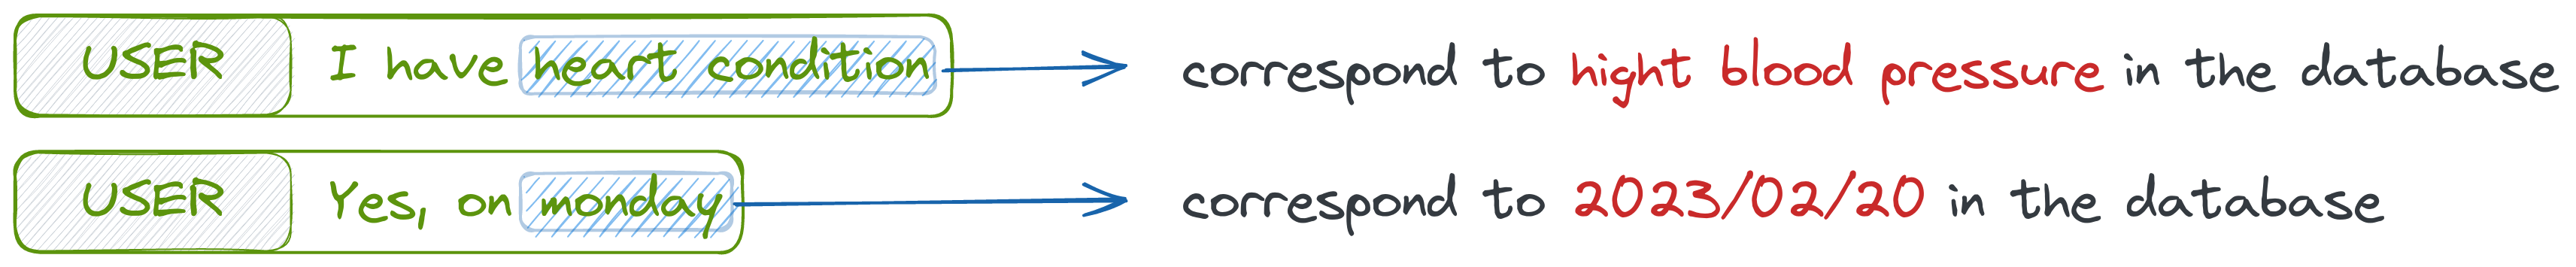
\includegraphics[width=1.\textwidth]{media/in_context_el.png}
        \label{fig:my_label}
    \end{figure}
    
\end{frame}
\begin{frame}{Entity Linking}
 
             For entity linking mostly depends on the domain  or the Database, different approaches can be envisioned
            \begin{itemize}
                \item Distance between mentions and entities (token/entity)
                \item specific ontologies (for instance in medical domain)
            \end{itemize}
        \begin{figure}
            \centering
            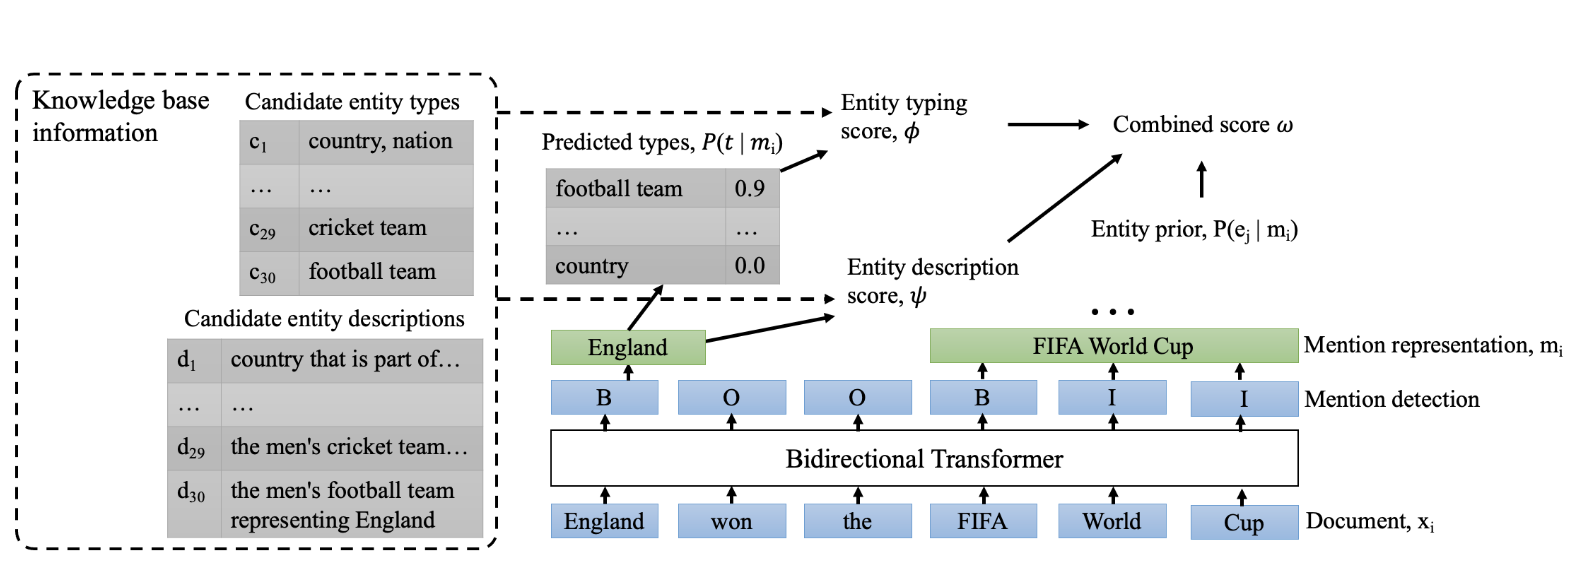
\includegraphics[width=0.7\textwidth]{media/refined.png}
            \caption{The ReFinED approach for entity linking basing on the distance of contextual embedding and both entity\_type and description of the entity \cite{ayoola-2022-refined}}
            \label{fig:refined}
        \end{figure}
\end{frame}
\begin{frame}
       \begin{columns}
        \begin{column}{0.6\textwidth}
    \begin{block}{Contextual undertanding}
        Often done by the \textbf{D}ialogue \textbf{S}tate \textbf{T}racking

        \begin{itemize}
            \item Knowledge Based approaches  \cite{llanos-etal-2016-managing}

            \item Neural Networks
            \begin{itemize}
                \item LSTM encoding jointly previous utterances \cite{Hori2015ContextSS}
                \item Memory Network \cite{chen2016end-to-end}
                \item Transformer with jointly encoded utterances (most of today approaches) \cite{gao-2019-bert}
                \item Transformer based prompt (generative) \cite{lee-etal-2021-dialogue}
            \end{itemize}
%             "BERT-DST: Scalable End-to-End Dialogue State Tracking with Bidirectional Encoder Representations from Transformer", Efficient Dialogue State Tracking by Masked Hierarchical Transformer, Multi-Domain Dialogue State Tracking – A Purely Transformer-Based
% Generative Approach
        \end{itemize}
    \end{block}
        \end{column}
        \begin{column}{0.4\textwidth}
            \begin{figure}
                \centering
                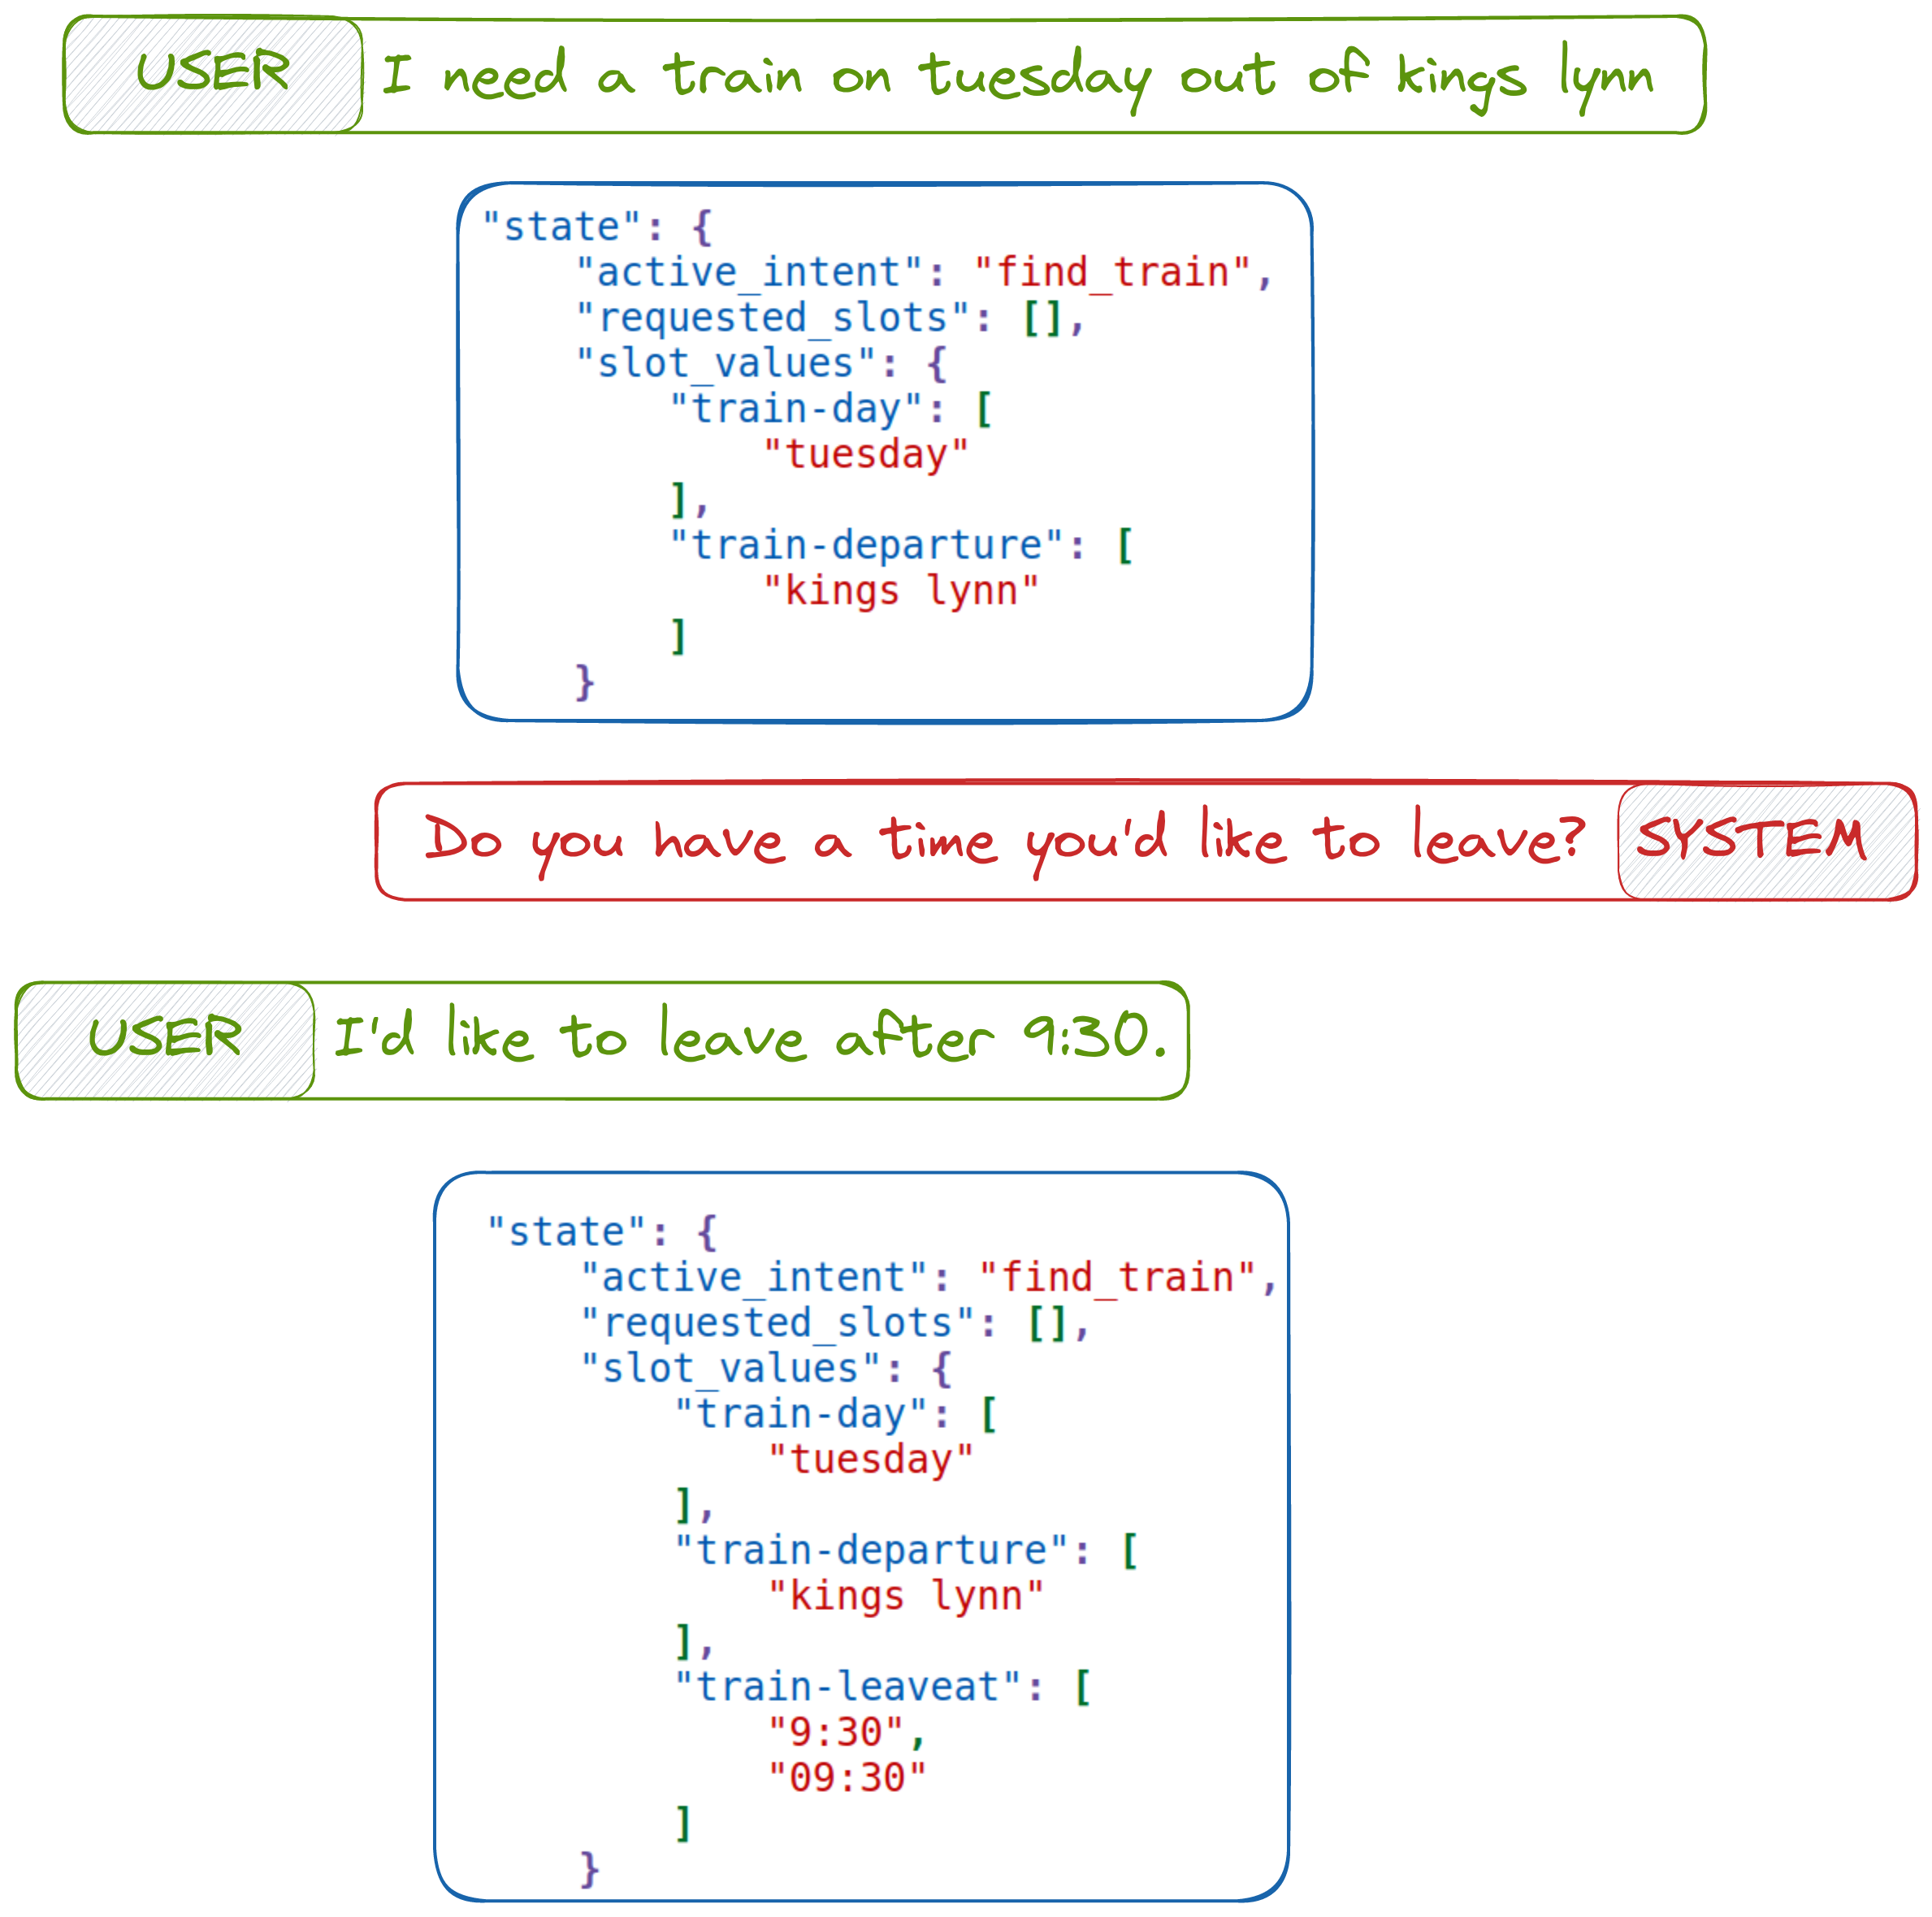
\includegraphics[width=1.\textwidth]{media/update_dst.png}

            \end{figure}
        \end{column}
    \end{columns}


\end{frame}
\begin{frame}{DM : Dialogue state model}
    \begin{block}{Dialiog State Tracking:}
        Provide a representation of what user want  at each utterances \cite{henderson-2015-machine} : 
        \begin{itemize}
            \item Using a set of slots type and value (see previous approaches)
            \item Using vector (e.g one hot vector) \cite{baud-2023-repondre}% lyon chatbot
            \item Update the information (the state vector or pairs of slots type/value)
        \end{itemize}
        Decision is then made on current state of the dialogues... 
    \end{block}
\end{frame}
\begin{frame}{DM and Dialogue control}
    \begin{columns}
        \begin{column}{0.5\textwidth}
            \begin{block}{Objectives:}
                Dialogue control has to decide what is the next step using the user input and the current state. For instance :
                \begin{itemize}
                    \item Asking new information (e.g. for booking "number of peoples", "times" ...)
                    \item Clarrify the the user's input/intent
                    \item giving information to the user
                    \item update the KB or database 
                \end{itemize}
            \end{block}
            We call this set of information the \textbf{D}alogue \textbf{A}ct (\texttt{DA})
        \end{column}
        \begin{column}{0.5\textwidth}
            \begin{figure}
                \centering
                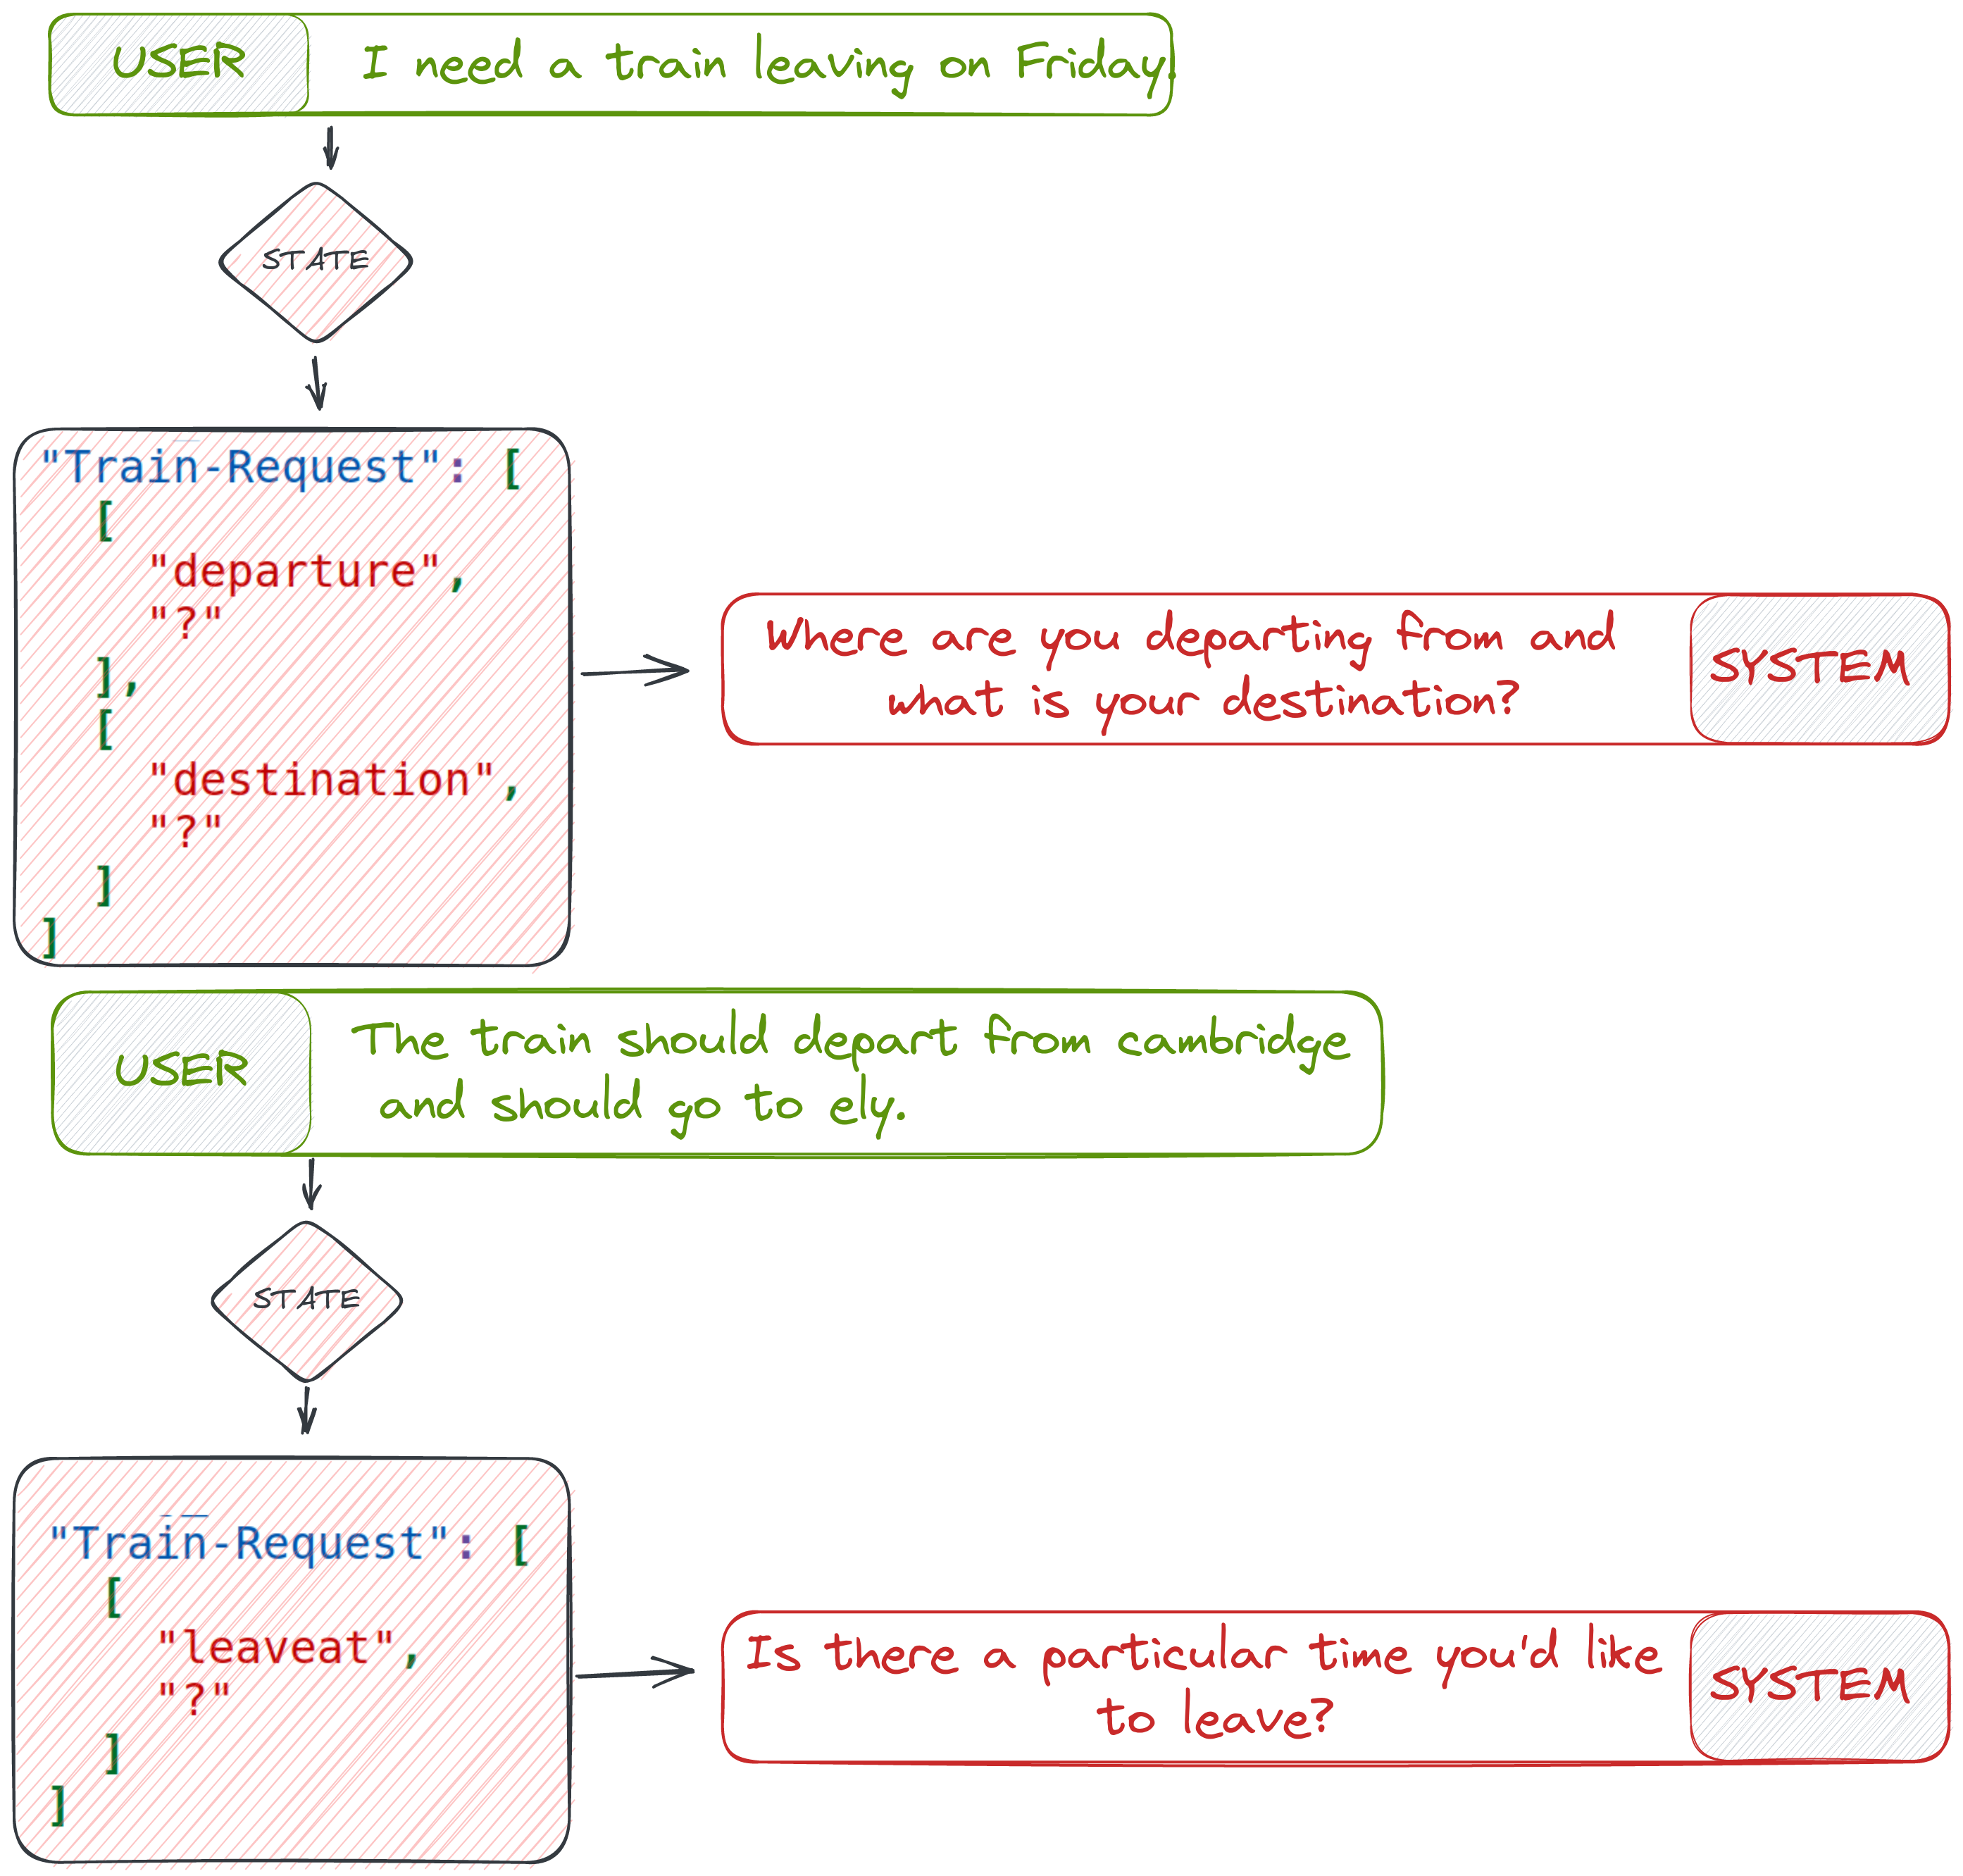
\includegraphics[width=1.\textwidth]{media/act.png}
            \end{figure}
        \end{column}
    \end{columns}
\end{frame}

\begin{frame}{DM and Dialogue control : Graph}
    \begin{columns}
        \begin{column}{0.5\textwidth}
            \begin{block}{Finite state automata}
                \begin{itemize}
                    \item Nodes represent the question of the systems
                    \item transition represent answers
                    \item The graph specifies all legal dialogues
                \end{itemize}
            \end{block}
            \begin{block}{Pros and cons}
                \begin{itemize}
                    \item Limited number of interactions
                    \item Used in  simple tasks and structured domain (few slots and number of values)
                    \item Cannot manage complex dialogues states
                \end{itemize}
                (In the application we will use this kind of approach!!!)
            \end{block}
        \end{column}
        \begin{column}{0.5\textwidth}
            \begin{figure}
                \centering
                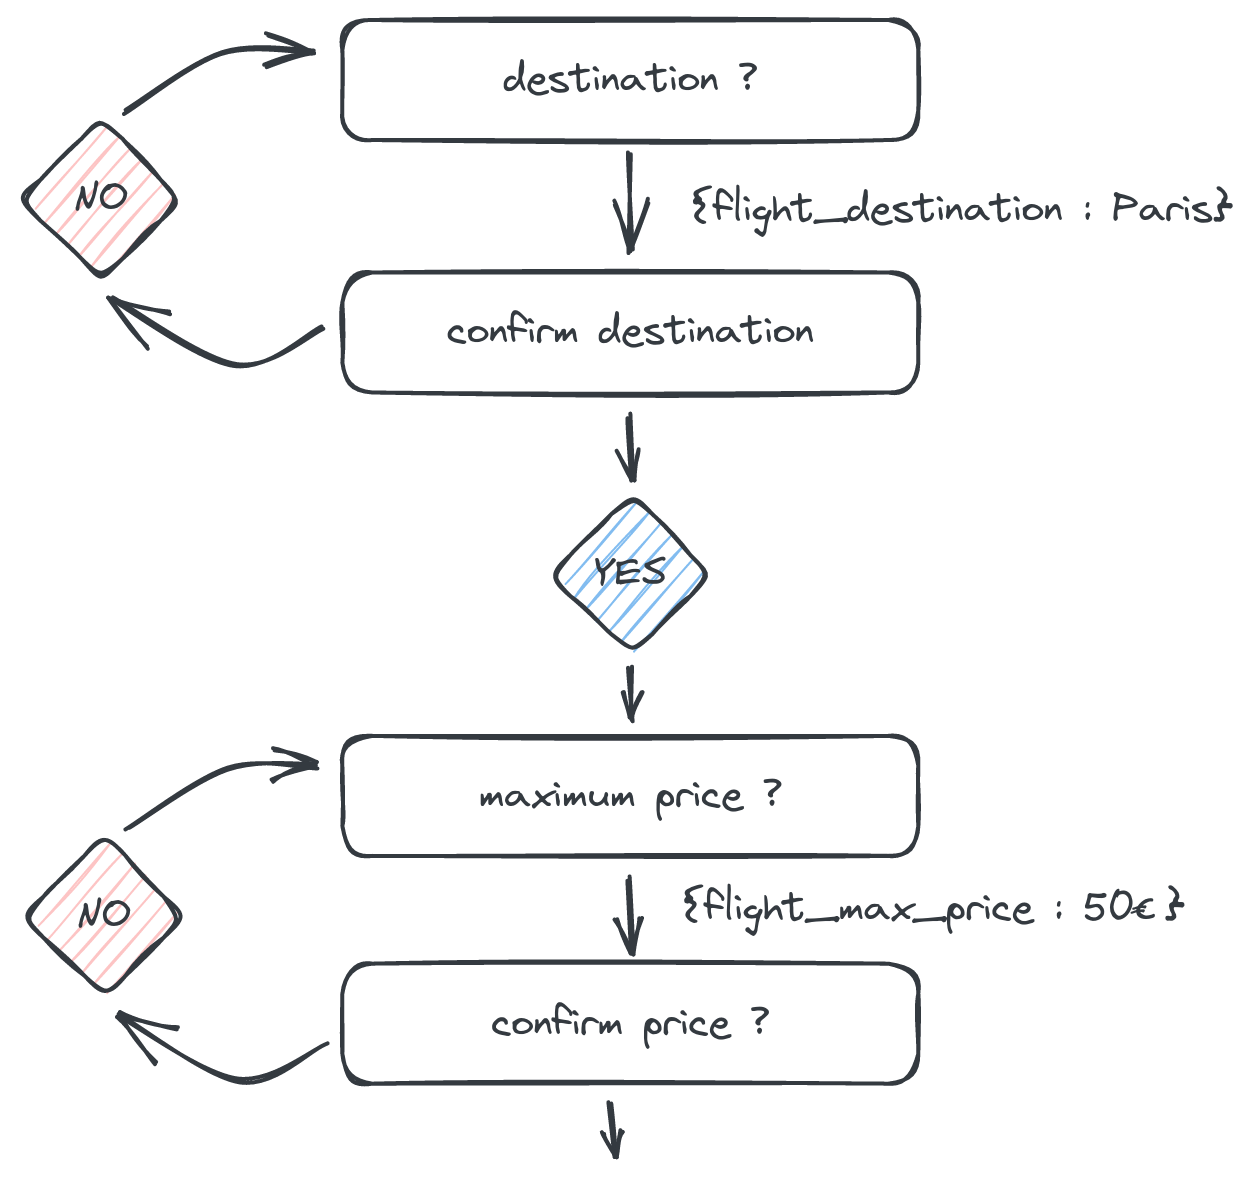
\includegraphics[width=1.\textwidth]{media/automata.png}
            \end{figure}
        \end{column}
    \end{columns}
    

\end{frame}

\begin{frame}{DM and Dialogue control : Frame based}
    \begin{columns}
        \begin{column}{0.5\textwidth}
            \begin{block}{Frame-based approaches}
                \begin{itemize}
                    \item A frame is a set of slots (no constraint on the utterance order of the user)
                    \item Possible to have many frames as substasks and more complex frames

                \end{itemize}
            \end{block}
            \begin{block}{How does it works}
                \begin{itemize}
                    \item A frame represents what the system has to solve
                    \item The slots  are filled  with values from user utterance
                \end{itemize}
            \end{block}
        \end{column}
        \begin{column}{0.5\textwidth}
            \begin{figure}
                \centering
                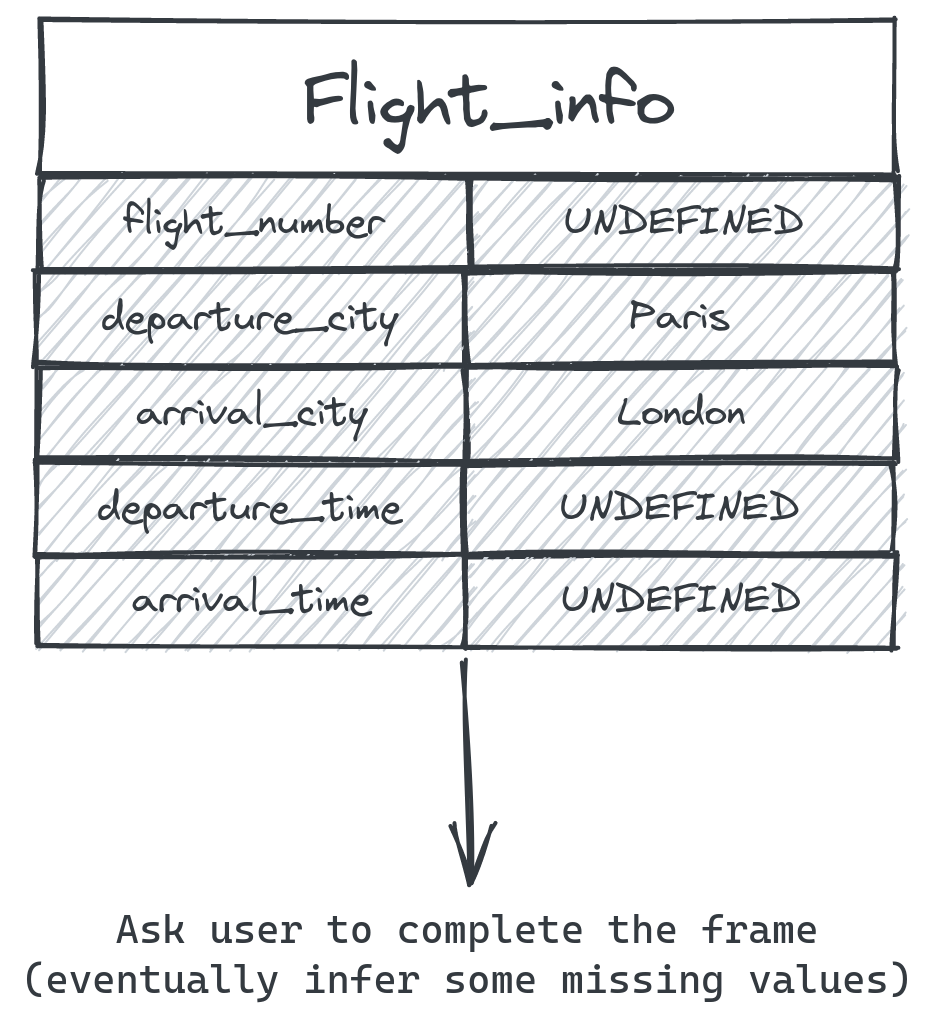
\includegraphics[width=.8\textwidth]{media/frame.png}
            \end{figure}
        \end{column}
    \end{columns}
\end{frame}

\begin{frame}{DM and Dialogue control : Policy Based and reinforcement learning}

    \begin{columns}
        \begin{column}{0.5\textwidth}
            \begin{block}{Reinforcement Learning}
                Learning to take decision/action 
                \begin{itemize}
                    \item Take a decision  given a (dialogue) state 
                    \item State are modelled with 
                        \begin{itemize}
                            \item \textbf{MDP:} Markov Decision Process \cite{levin-2000-stochastic}
                            \item \textbf{POMDP:} Partially Observable Markov Decision Process \cite{Young2006USINGPF}
                        \end{itemize}
                    \item use a reinforce strategy, dialogue policy optimization
                \end{itemize}
            \end{block}

        \end{column}
        \begin{column}{0.5\textwidth}
                        \begin{block}{Pros and Cons}
                \begin{itemize}
                    \item Not necessarly need to review all possibilities 
                    \item Data is needed 
                \end{itemize}
            \end{block}
        \end{column}
    \end{columns}
\end{frame}

\begin{frame}{DM and Dialogue control : End-to-end \& Neural networks}
    \begin{columns}
        \begin{column}{0.5\textwidth}
                \begin{block}{Neural Approaches}
                    Relatively a new kind of approach \cite{wen-2016-network}
                    \begin{itemize}
                        \item Learn to map history/dialogue slots (on previous and current utterance) to an answer 
                        \item Hybrid approaches \cite{williams-etal-2017-hybrid, HAM201980}
                        \item Fully generative approach (feed with history) \cite{yang_2021_toward}(transformer)
                    \end{itemize}
                \end{block}
            
            \end{column}
        \begin{column}{0.5\textwidth}
                        \begin{block}{Pros and Cons}
                        Mostly the same as RL approaches
                \begin{itemize}
                    \item Not necessarly need to review all possibilities 
                    \item Huge amount of data is needed to train (particularly for transformer)
                \end{itemize}
            \end{block}
        \end{column}
    \end{columns}
\end{frame}


\begin{frame}{DM and Dialogue Control : Strengths and weakness}
    \begin{columns}
        \begin{column}{0.5\textwidth}
                
                \begin{block}{Rule based approaches}
                    Often for Automata and frame based approaches 

                    \begin{block}{Strength}
                        \begin{itemize}
                            \item Easy to interpret 
                            \item Few data needed
                        \end{itemize}   
                        Those approaches are mostly used in industry
                    \end{block}
                    \begin{alertblock}{Weakness}
                        \begin{itemize}
                            \item May be difficult to maintain
                            \item Long and time consuming to maintaining rules (how to address most of possibilities) for complex systems
                        \end{itemize}   
                    \end{alertblock}
                \end{block}
            
            \end{column}
        \begin{column}{0.5\textwidth}
            \begin{block}{Statistical and Neural approaches}
                For RL and Neural Networks
                    \begin{block}{Strength}
                        \begin{itemize}
                            \item Based on data (more natural response)
                            \item Do not need to give explicitly the different cases
                        \end{itemize}   
                    \end{block}
                    \begin{alertblock}{Weakness}
                        \begin{itemize}
                            \item Data needed (huge amount particularly for end to end)
                            \item Debugging and interpretation is often difficult
                        \end{itemize}   
                    \end{alertblock}

            \end{block}
        \end{column}
    \end{columns}
    
\end{frame}
\begin{frame}{Generate}
      \begin{figure}
        \centering
        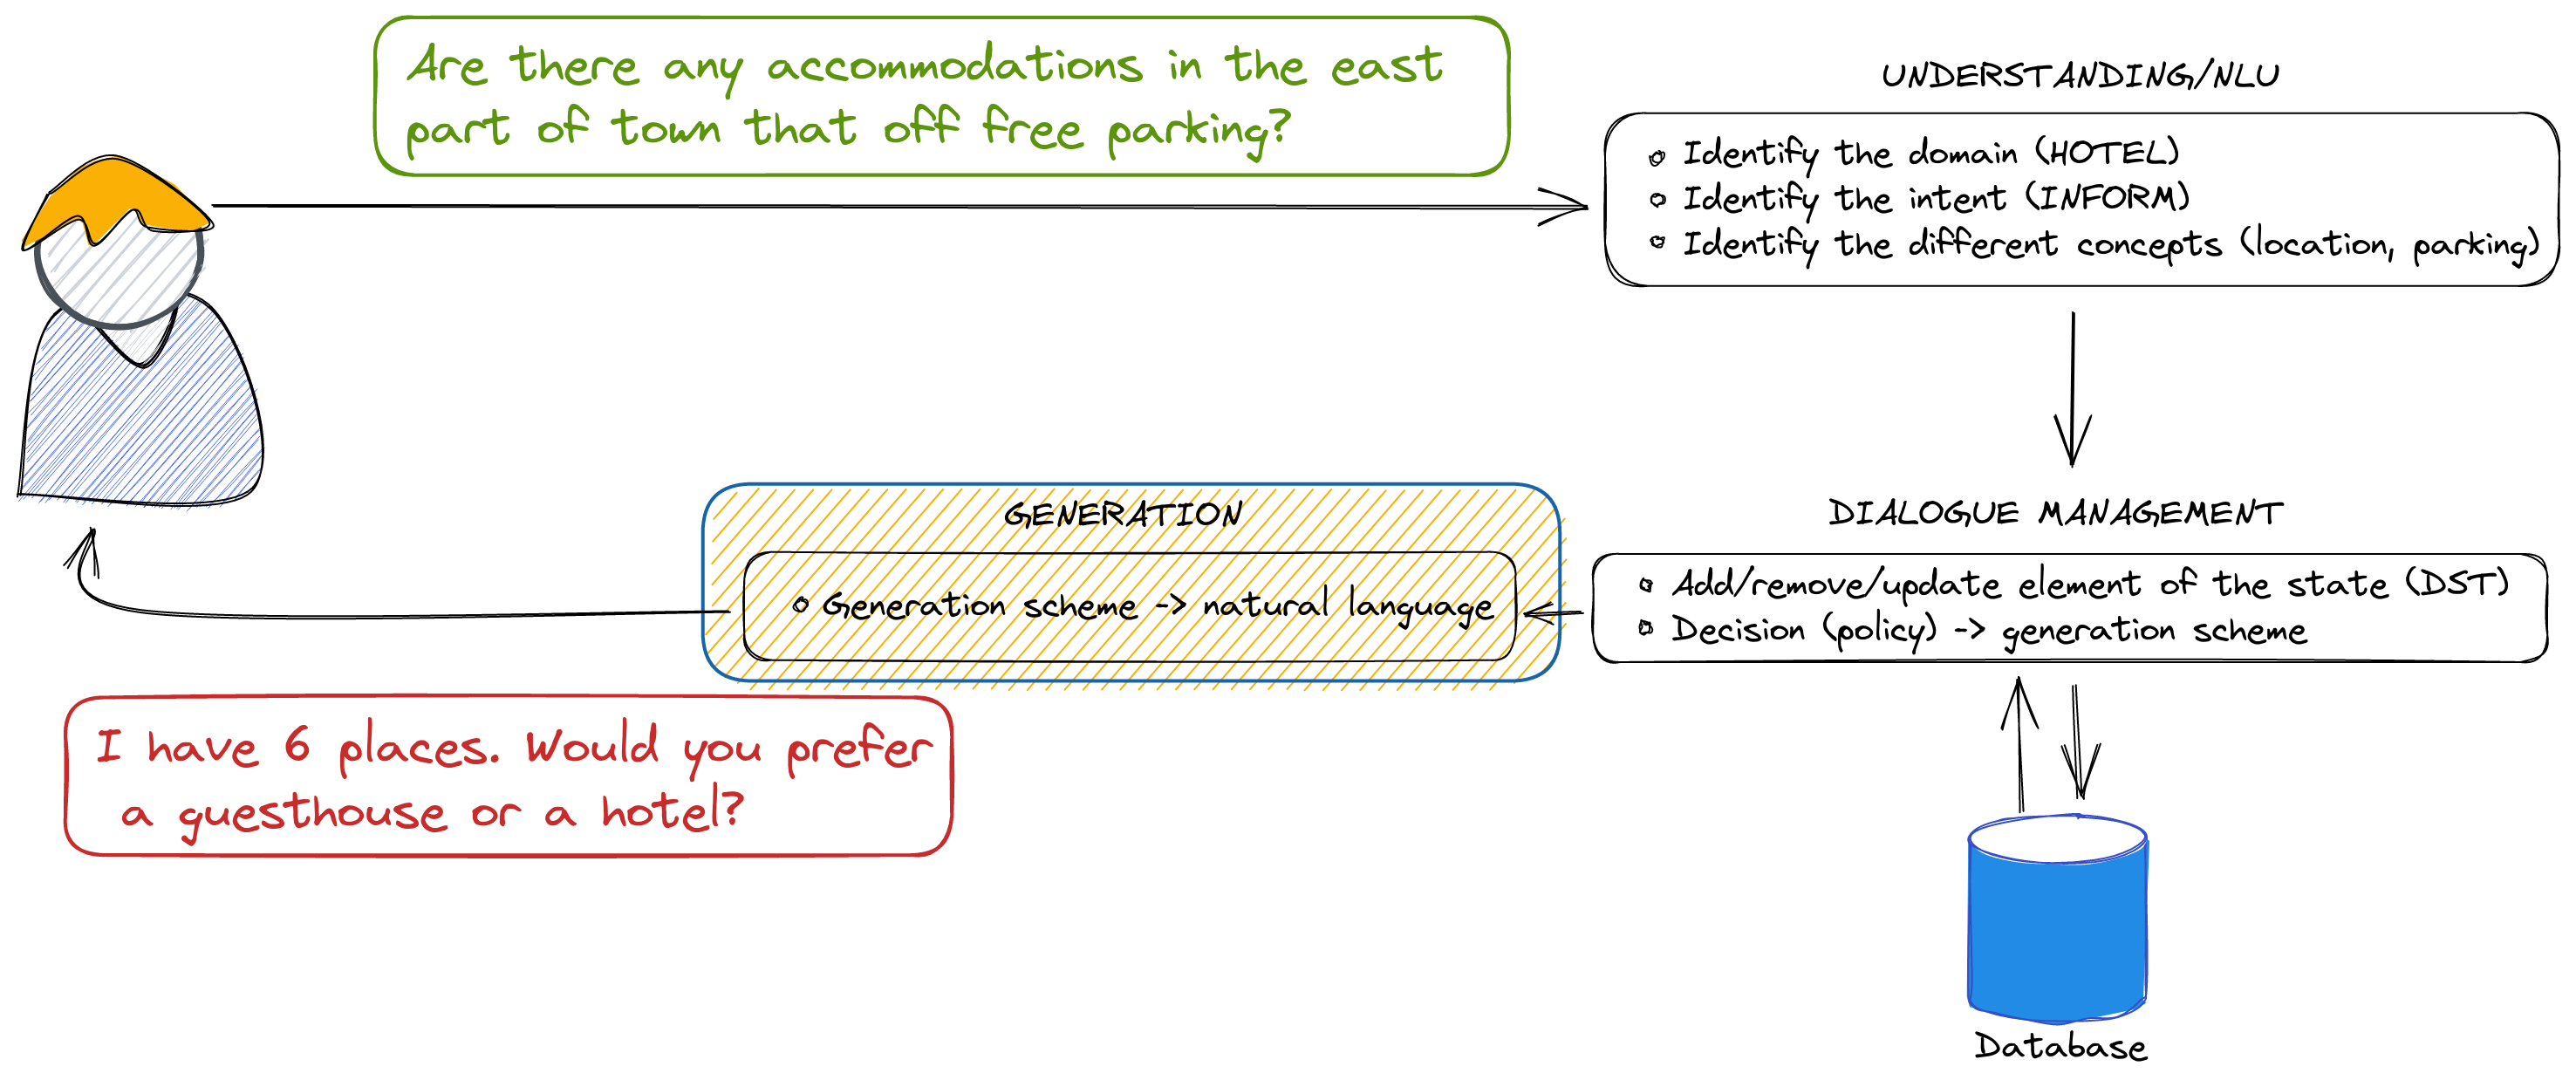
\includegraphics[width=1.\textwidth]{media/dialogue_task_complete_gen.png}
    \end{figure}
    
\end{frame}

\begin{frame}{NLG}
    \begin{block}{Objectives:}
        Transform information returned by DM and generate an answer. Decide how to present the newt utterances words.
        \begin{itemize}
            \item Take DM informations such next requested informations or confirmation (asked previously by user)
            \item Decide how and what to say
        \end{itemize}
    \end{block}
    \begin{block}{Different approaches: }
        \begin{itemize}
            \item Template based : \\
                \textbf{Exemple} : You have a train leaving at \$confirm\_departure\_value (using information of the frame)
            \item Statistical Models such as Neural Networks such as Transformer models \cite{peng-etal-2020-shot} (using DA)

        \end{itemize}
    \end{block}
\end{frame}
\begin{frame}{Different ressources}
\begin{columns}
    \begin{column}{0.5\textwidth}
        \begin{block}{Libraries and software}
            \begin{itemize}
                \item RASA (create a conversationnal systems)  \footnote{https://rasa.com/blog/attention-dialogue-and-learning-reusable-patterns/}
                \item ConvLab2, Convlab3 \footnote{\url{https://github.com/ConvLab/ConvLab-3}}
            \end{itemize}
        \end{block}

    \end{column}
    \begin{column}{0.5\textwidth}
        \begin{block}{Corpus and dataset (non-exhaustive)}
            \begin{itemize}
                \item \textbf{ATIS:}  Airline Travel Information Systems (exists in multi lingual settings)
                \item \textbf{MultiWOZ:} a multi domain dataset (accomodation, taxi, restaurant etc..) for booking or requesting informations
                \item \textbf{Microsoft Dialogue Challenge:} Multi-domain (movie-ticket, restaurant, taxi)
                \item \textbf{SNIPS: } Multi-domain (alarm, weather...)
                \item \textbf{PVDial} : Medical dialogue (in french) \footnote{\url{https://pvdial.limsi.fr/}}
            \end{itemize}
        \end{block}
    \end{column}
\end{columns}
\end{frame}

\begin{frame}{A small recap}
    \begin{columns}
        \begin{column}{0.6\textwidth}
            \begin{block}{Task-oriented systems: }
                A task oriented dialogues syste is a complex system that aims to provide specific informations an a subset of domains. In most cases it rely on a KB or a relationnal database where to find/update informations. The pipeline require different components:
                \begin{itemize}
                    \item (ASR) \textcolor{orange}{\textbf{A}utomatic \textbf{S}peech \textbf{R}ecognition}
                    \item (NLU) \textbf{N}atural \textbf{L}anguage \textbf{U}nderstanding 
                    \item (DM) \textbf{D}ialogue \textbf{M}anagement (state tracking and dialogue control)
                    \item (NLG) \textbf{N}atural \textbf{L}anguage \textbf{G}eneration
                    \item (TS)  \textcolor{orange}{\textbf{T}ext to \textbf{S}peech}
                \end{itemize}
            \end{block}
        \end{column}
        \begin{column}{0.4\textwidth}
            \begin{block}{Approaches:}
                For each componenents a  variety of approaches exists such as rules with explicit domain knowledge or statistical and neural approaches(generative/extractive).
            \end{block}
        \end{column}
    \end{columns}
\end{frame}

\section{Chit-Chat and Purely Conversational Systems}
\begin{frame}{Chit-chat Bot}
\begin{columns}
        \begin{column}{0.5\textwidth}
            \begin{block}{Objectives:}
                \begin{itemize}
                    \item General conversation abilities
                    \item Generate most appropriate reaction given the context and the previous user utterance
                \end{itemize}
            \end{block}
            \begin{block}{What is needed:}
                \begin{itemize}
                    \item Huge collection of dialogs
                \end{itemize}
            \end{block}
        \end{column}
        \begin{column}{0.5\textwidth}
            \begin{figure}
                \centering
                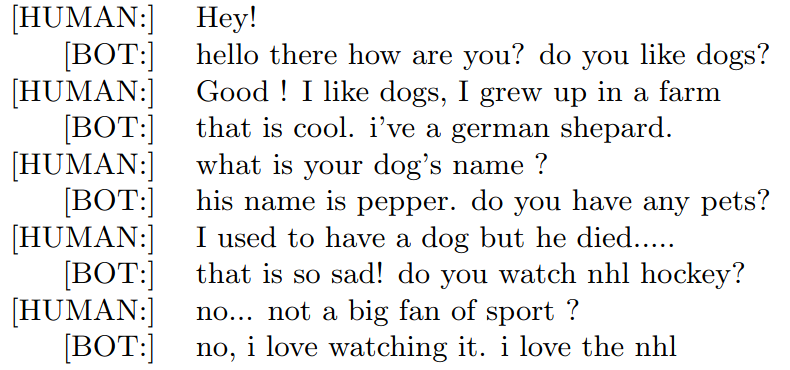
\includegraphics[width=1.\textwidth]{media/chichat_exemple.png}
                \caption{Extract of a dialogue for the Second Conversational Intelligence Challenge \cite{convaichallenge}}
                \label{fig:my_label}
            \end{figure}
        \end{column}
    \end{columns}
\end{frame}
\begin{frame}{Contextualize word in sentence: Seq2Seq with RNN}

    \begin{block}{Sequence to Sequence}
      \vspace{.1cm}
      {\footnotesize
        Model a sequence to sequence task with RNN :\\ 
        $\rightarrow $ Use \textit{``many to one''} variant to encode the input sequence\\
        $\rightarrow $ Use \textit{``one to many''} variant to generate a new sequence\\
      } 
    \end{block}

    \begin{figure}
      \centering
      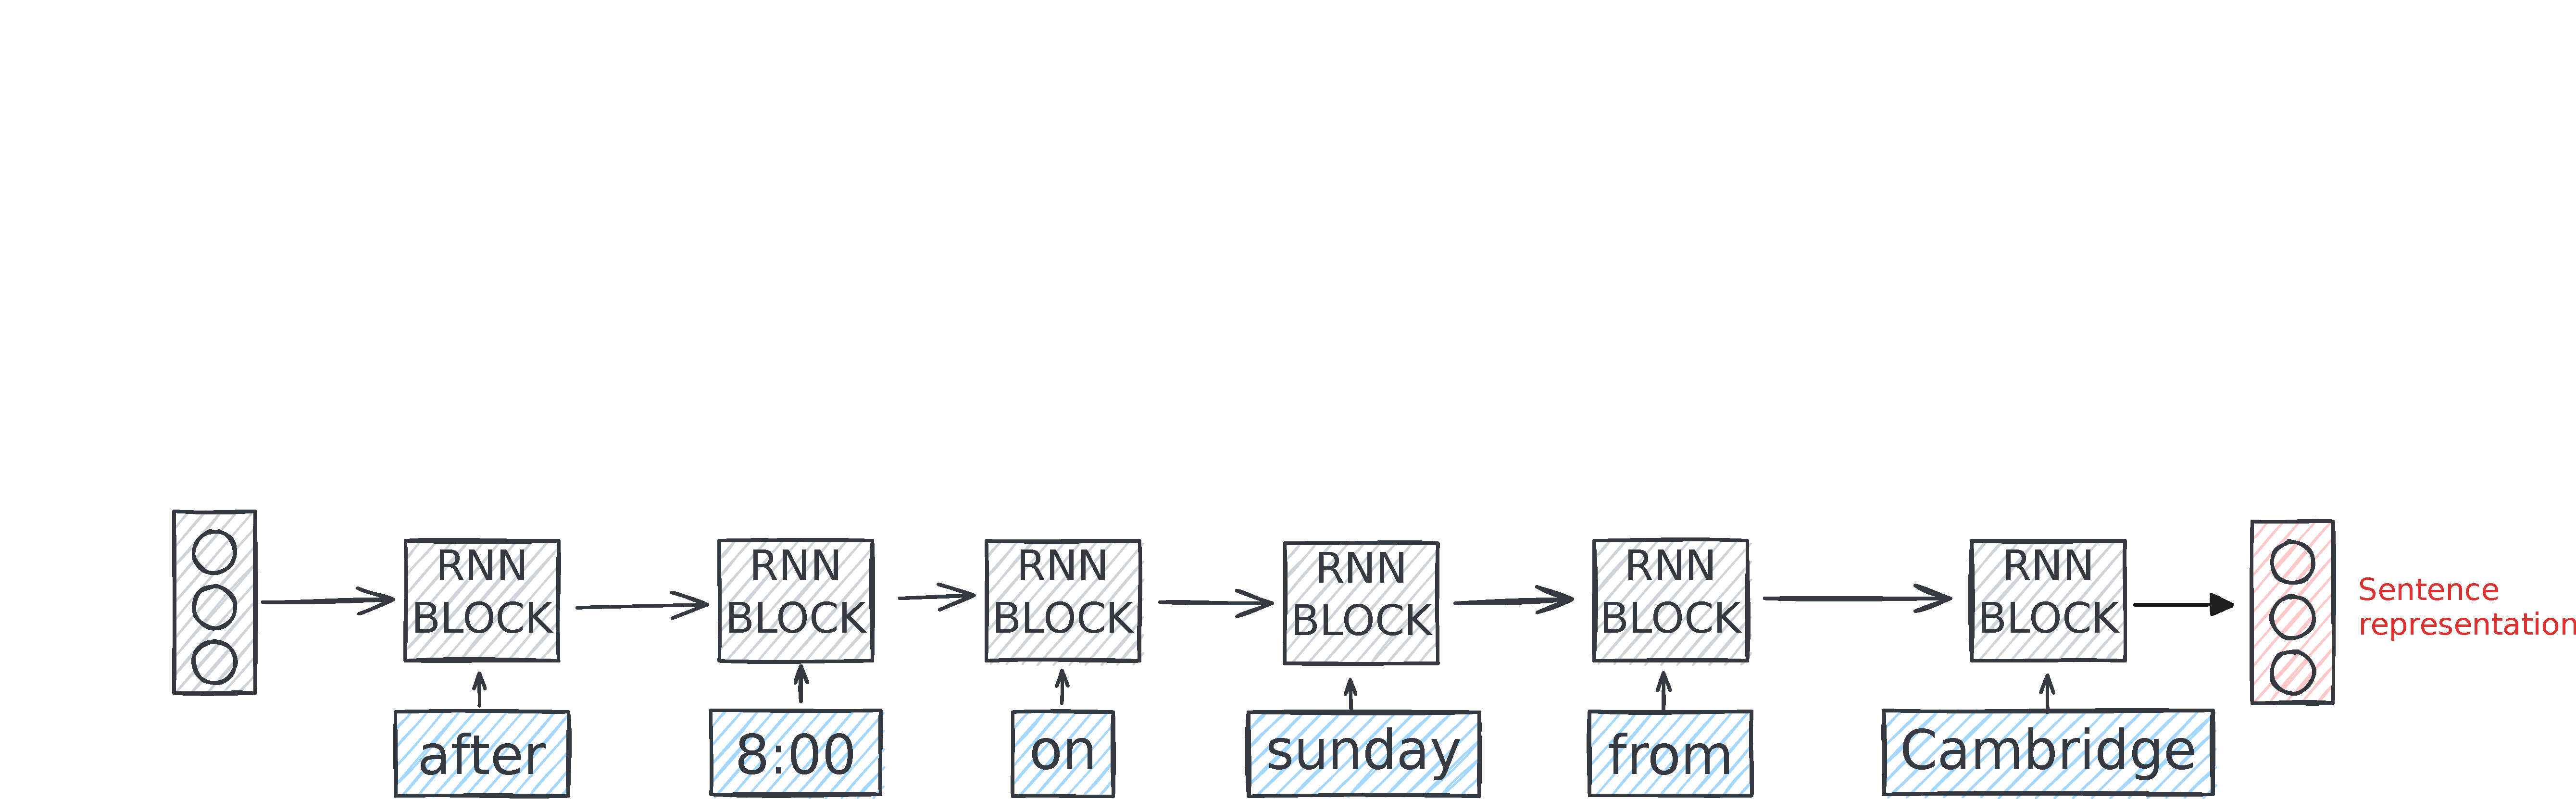
\includegraphics[width=1.\textwidth]{img/RNN-example-seq2seq-8.pdf}
    \end{figure}

    \phantom{\tiny \textbf{NB:} The \textit{EOS} word is a special word indicating the end of the sentence}

  \end{frame}

  \begin{frame}[noframenumbering]{Contextualize word in sentence: Seq2Seq with RNN}

    \begin{block}{Sequence to Sequence}
      \vspace{.1cm}
      {\footnotesize
        Model a sequence to sequence task with RNN :\\ 
        $\rightarrow $ Use \textit{``many to one''} variant to encode the input sequence\\
        $\rightarrow $ Use \textit{``one to many''} variant to generate a new sequence\\
      } 
    \end{block}

    \begin{figure}
      \centering
      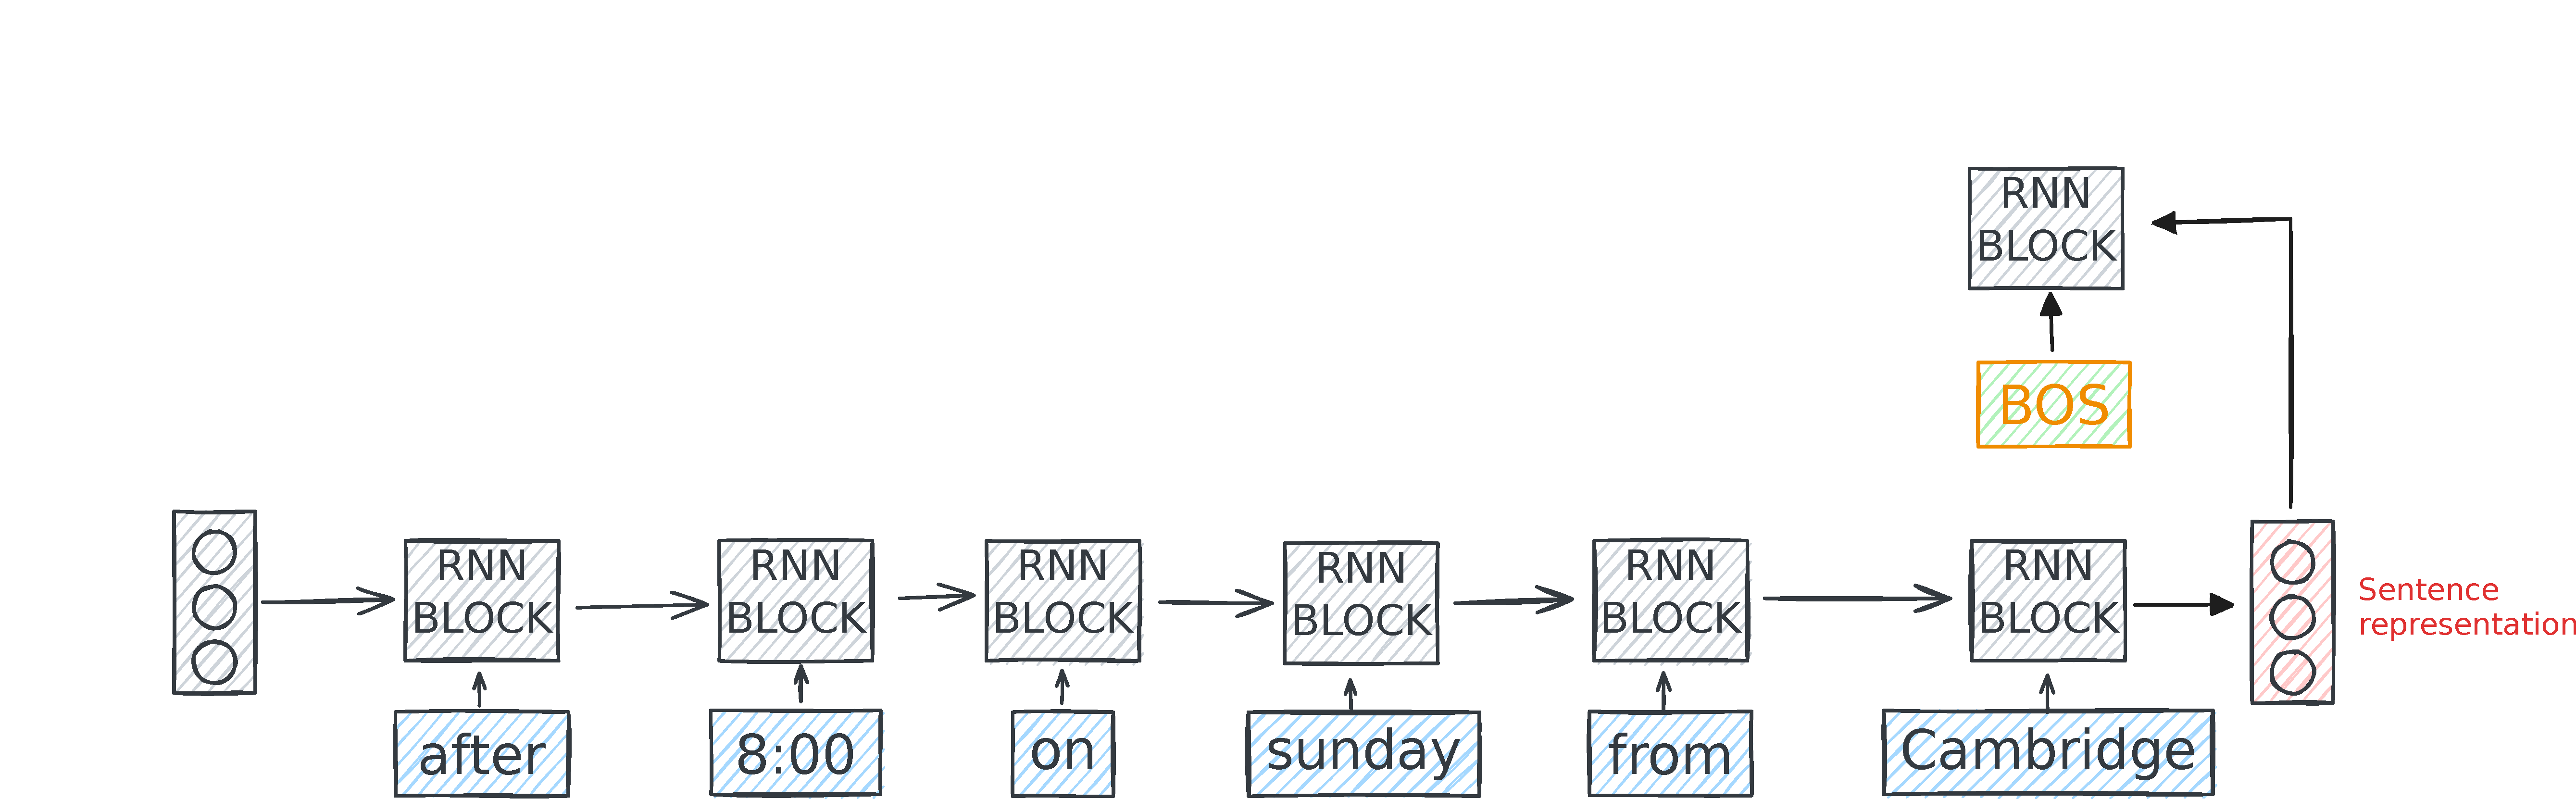
\includegraphics[width=1.\textwidth]{img/RNN-example-seq2seq-7.pdf}
    \end{figure}

    \phantom{\tiny \textbf{NB:} The \textit{EOS} word is a special word indicating the end of the sentence}

  \end{frame}

  \begin{frame}[noframenumbering]{Contextualize word in sentence: Seq2Seq with RNN}

    \begin{block}{Sequence to Sequence}
      \vspace{.1cm}
      {\footnotesize
        Model a sequence to sequence task with RNN :\\ 
        $\rightarrow $ Use \textit{``many to one''} variant to encode the input sequence\\
        $\rightarrow $ Use \textit{``one to many''} variant to generate a new sequence\\
      } 
    \end{block}

    \begin{figure}
      \centering
      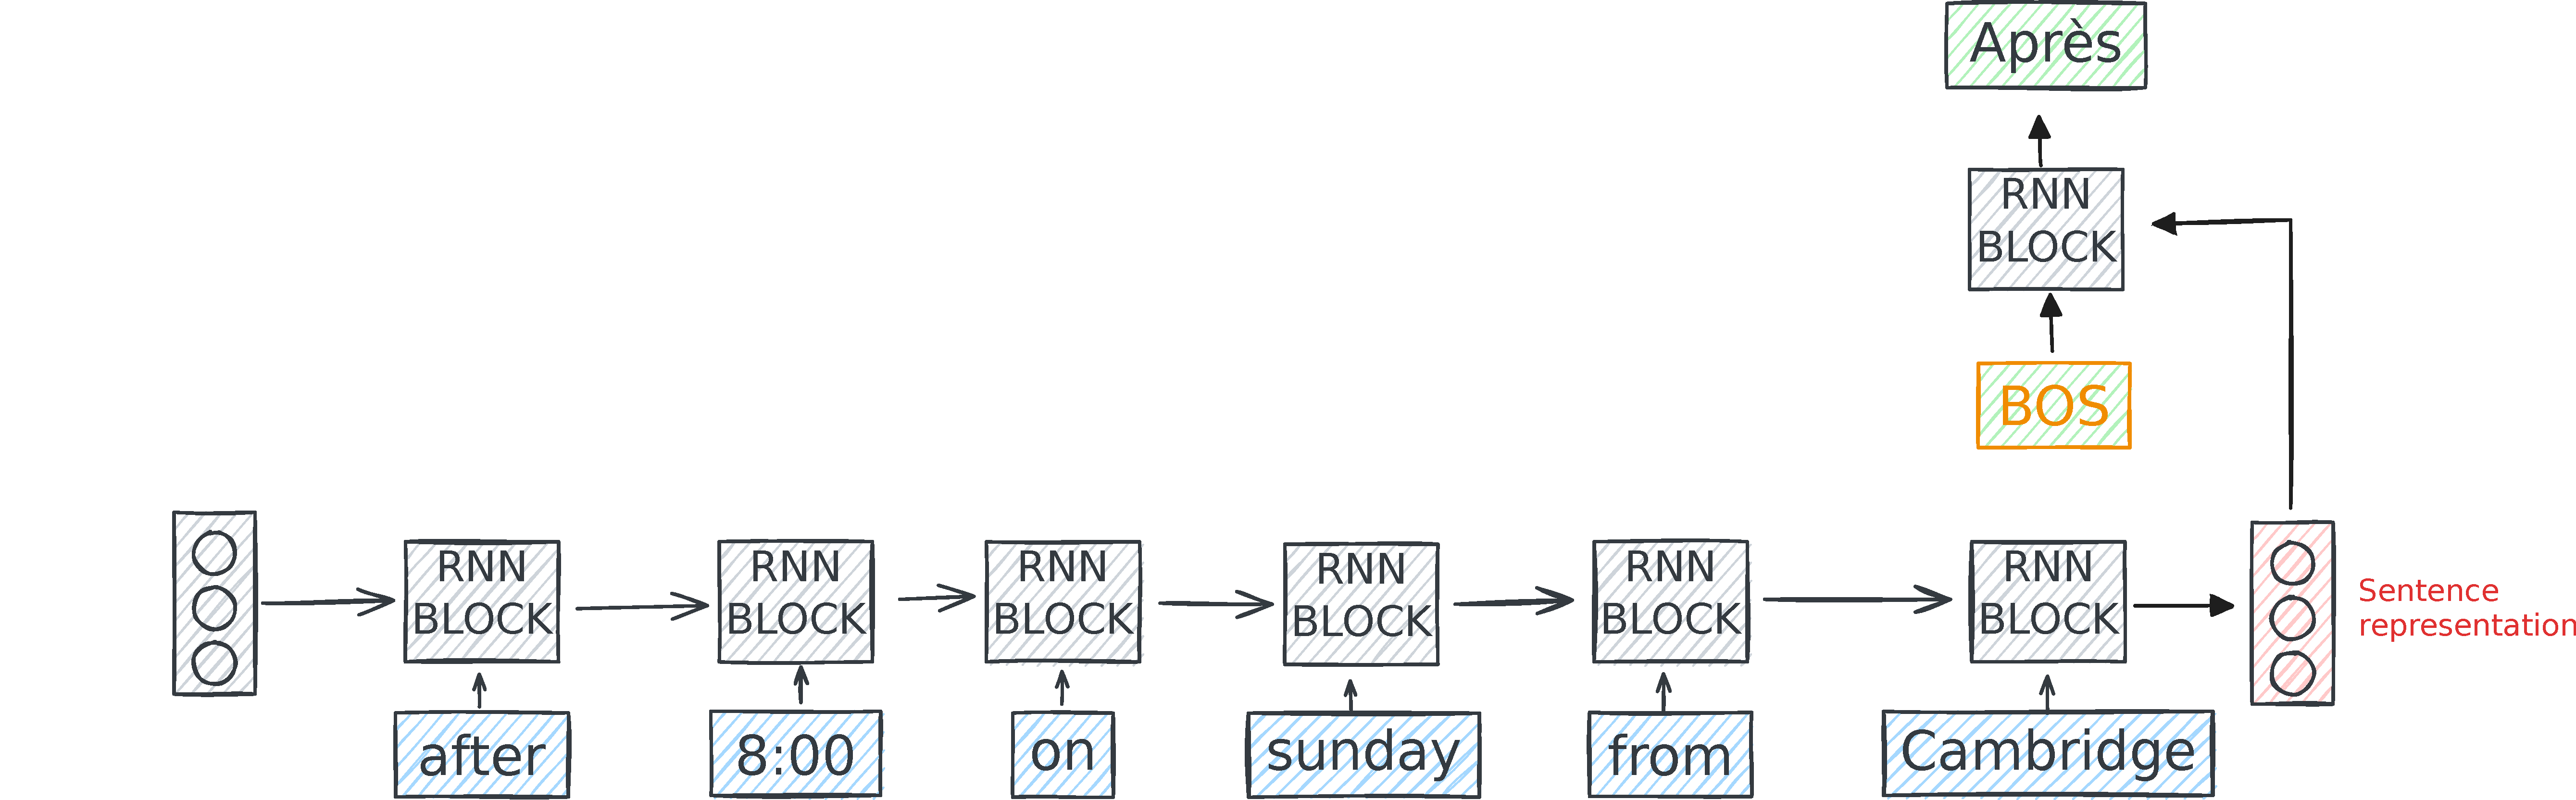
\includegraphics[width=1.\textwidth]{img/RNN-example-seq2seq-6.pdf}
    \end{figure}

    \phantom{\tiny \textbf{NB:} The \textit{EOS} word is a special word indicating the end of the sentence}

  \end{frame}

  \begin{frame}[noframenumbering]{Contextualize word in sentence: Seq2Seq with RNN}

    \begin{block}{Sequence to Sequence}
      \vspace{.1cm}
      {\footnotesize
        Model a sequence to sequence task with RNN :\\ 
        $\rightarrow $ Use \textit{``many to one''} variant to encode the input sequence\\
        $\rightarrow $ Use \textit{``one to many''} variant to generate a new sequence\\
      } 
    \end{block}

    \begin{figure}
      \centering
      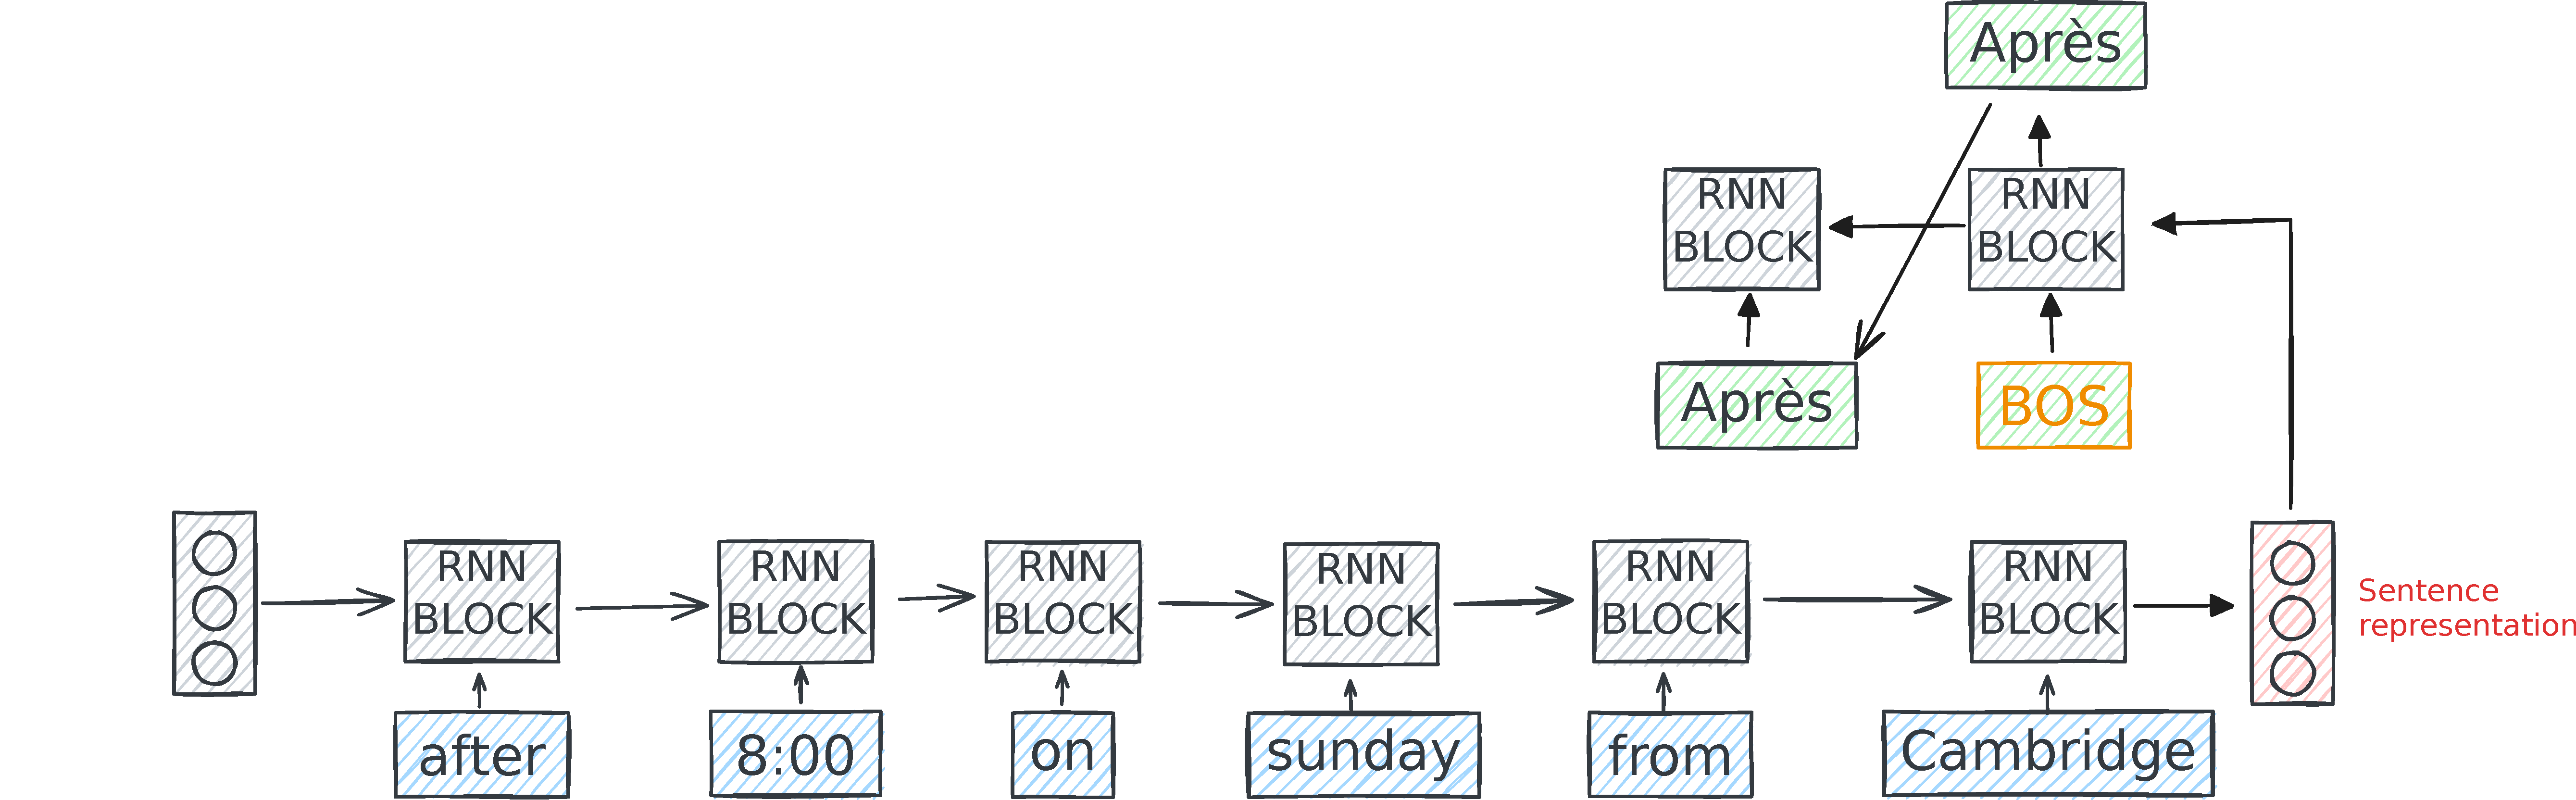
\includegraphics[width=1.\textwidth]{img/RNN-example-seq2seq-5.pdf}
    \end{figure}

    \phantom{\tiny \textbf{NB:} The \texttt{EOS} word is a special word indicating the End Of the Sentence}

  \end{frame}

  \begin{frame}[noframenumbering]{Contextualize word in sentence: Seq2Seq with RNN}

    \begin{block}{Sequence to Sequence}
      \vspace{.1cm}
      {\footnotesize
        Model a sequence to sequence task with RNN :\\ 
        $\rightarrow $ Use \textit{``many to one''} variant to encode the input sequence\\
        $\rightarrow $ Use \textit{``one to many''} variant to generate a new sequence\\
      } 
    \end{block}

    \begin{figure}
      \centering
      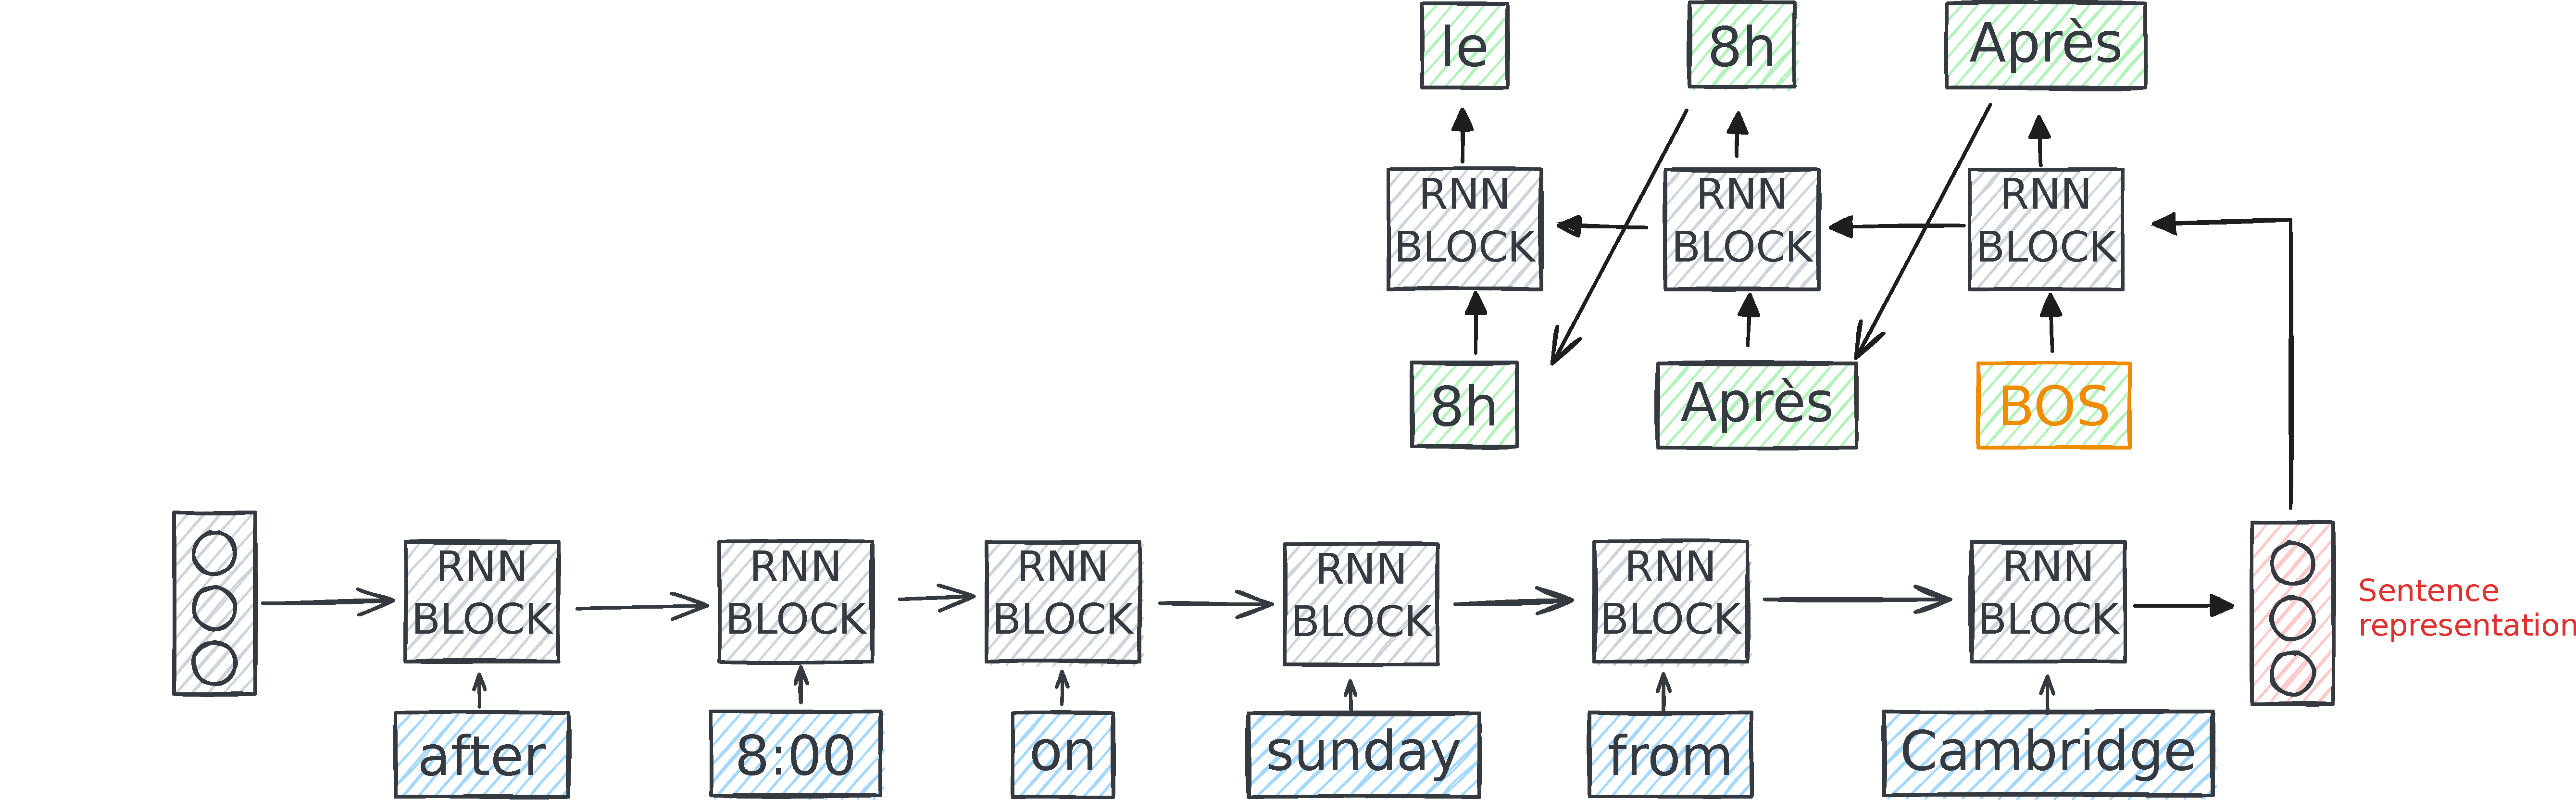
\includegraphics[width=1.\textwidth]{img/RNN-example-seq2seq-4.pdf}
    \end{figure}

    \phantom{\tiny \textbf{NB:} The \textit{EOS} word is a special word indicating the end of the sentence}

  \end{frame}

  \begin{frame}[noframenumbering]{Contextualize word in sentence: Seq2Seq with RNN}

    \begin{block}{Sequence to Sequence}
      \vspace{.1cm}
      {\footnotesize
        Model a sequence to sequence task with RNN :\\ 
        $\rightarrow $ Use \textit{``many to one''} variant to encode the input sequence\\
        $\rightarrow $ Use \textit{``one to many''} variant to generate a new sequence\\
      } 
    \end{block}

    \begin{figure}
      \centering
      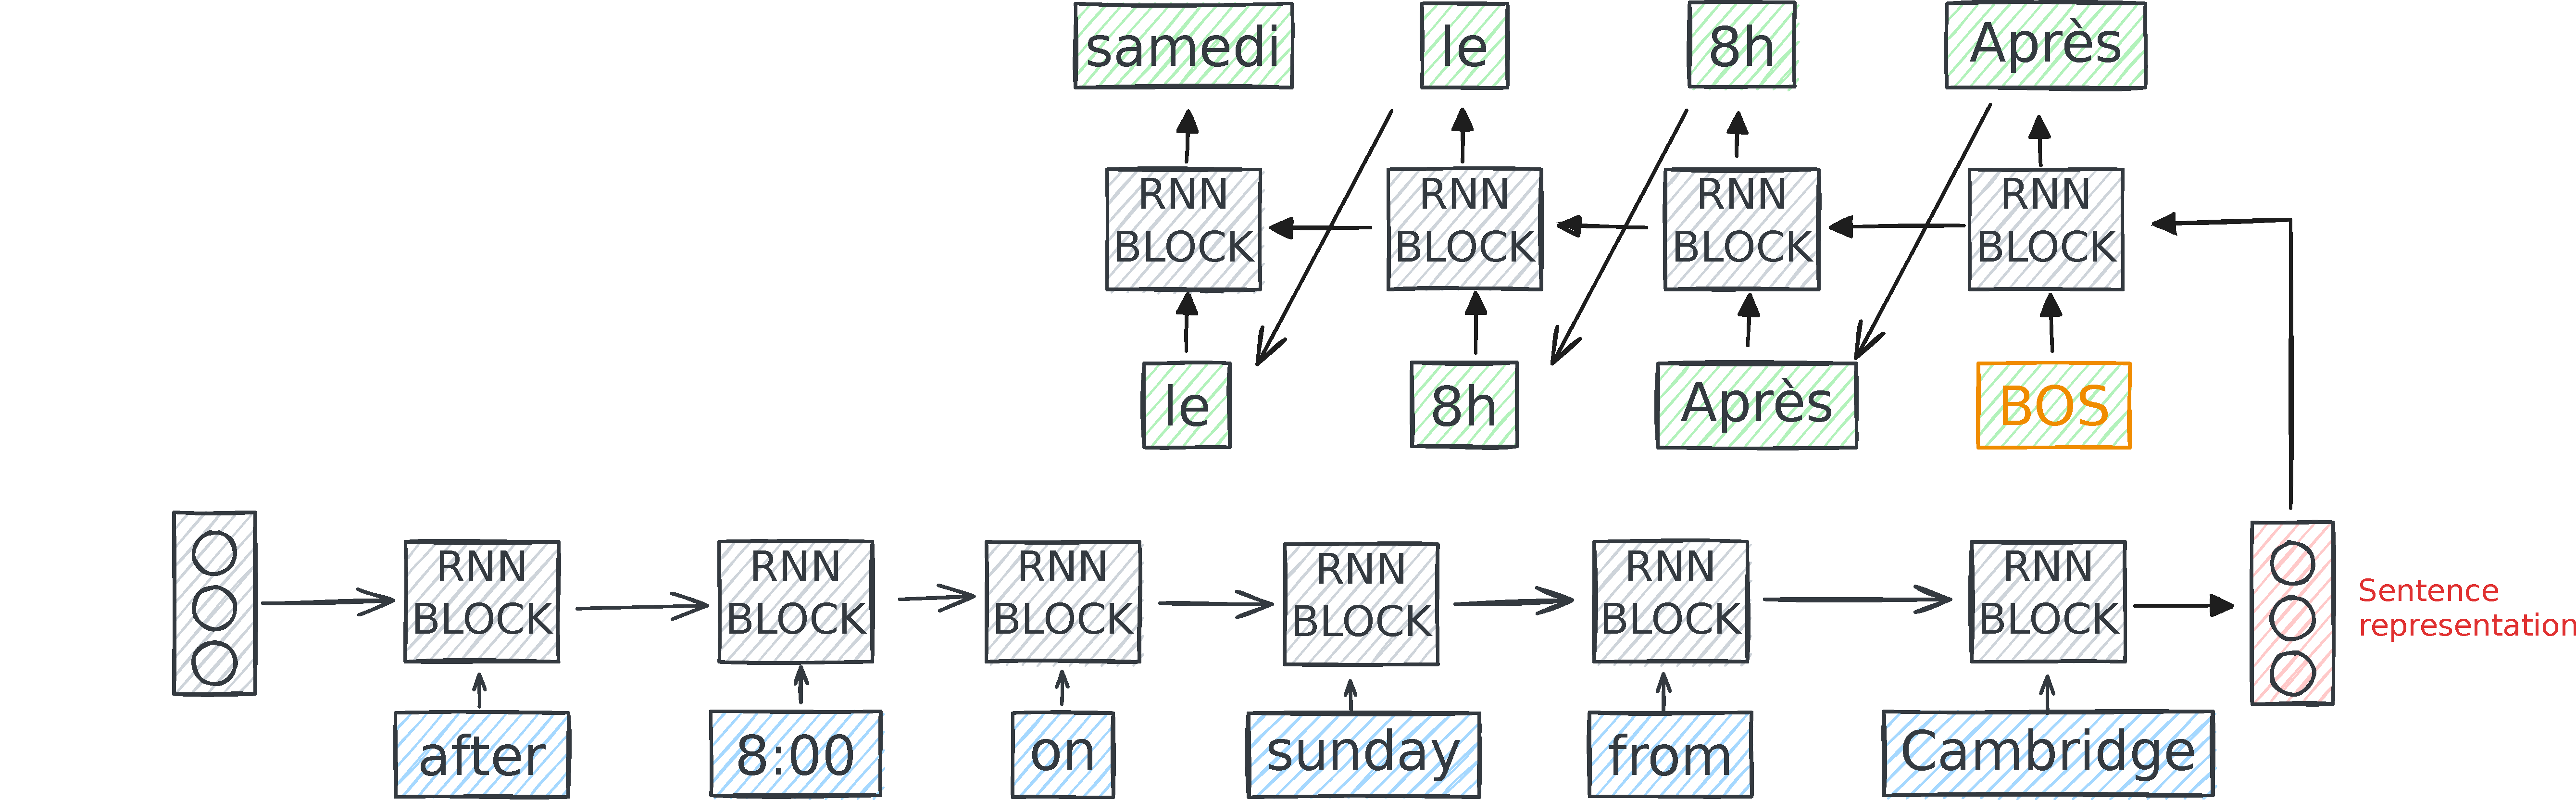
\includegraphics[width=1.\textwidth]{img/RNN-example-seq2seq-3.pdf}
    \end{figure}

    \phantom{\tiny \textbf{NB:} The \textit{EOS} word is a special word indicating the end of the sentence}

  \end{frame}

  \begin{frame}[noframenumbering]{Contextualize word in sentence: Seq2Seq with RNN}

    \begin{block}{Sequence to Sequence}
      \vspace{.1cm}
      {\footnotesize
        Model a sequence to sequence task with RNN :\\ 
        $\rightarrow $ Use \textit{``many to one''} variant to encode the input sequence\\
        $\rightarrow $ Use \textit{``one to many''} variant to generate a new sequence\\
      } 
    \end{block}

    \begin{figure}
      \centering
      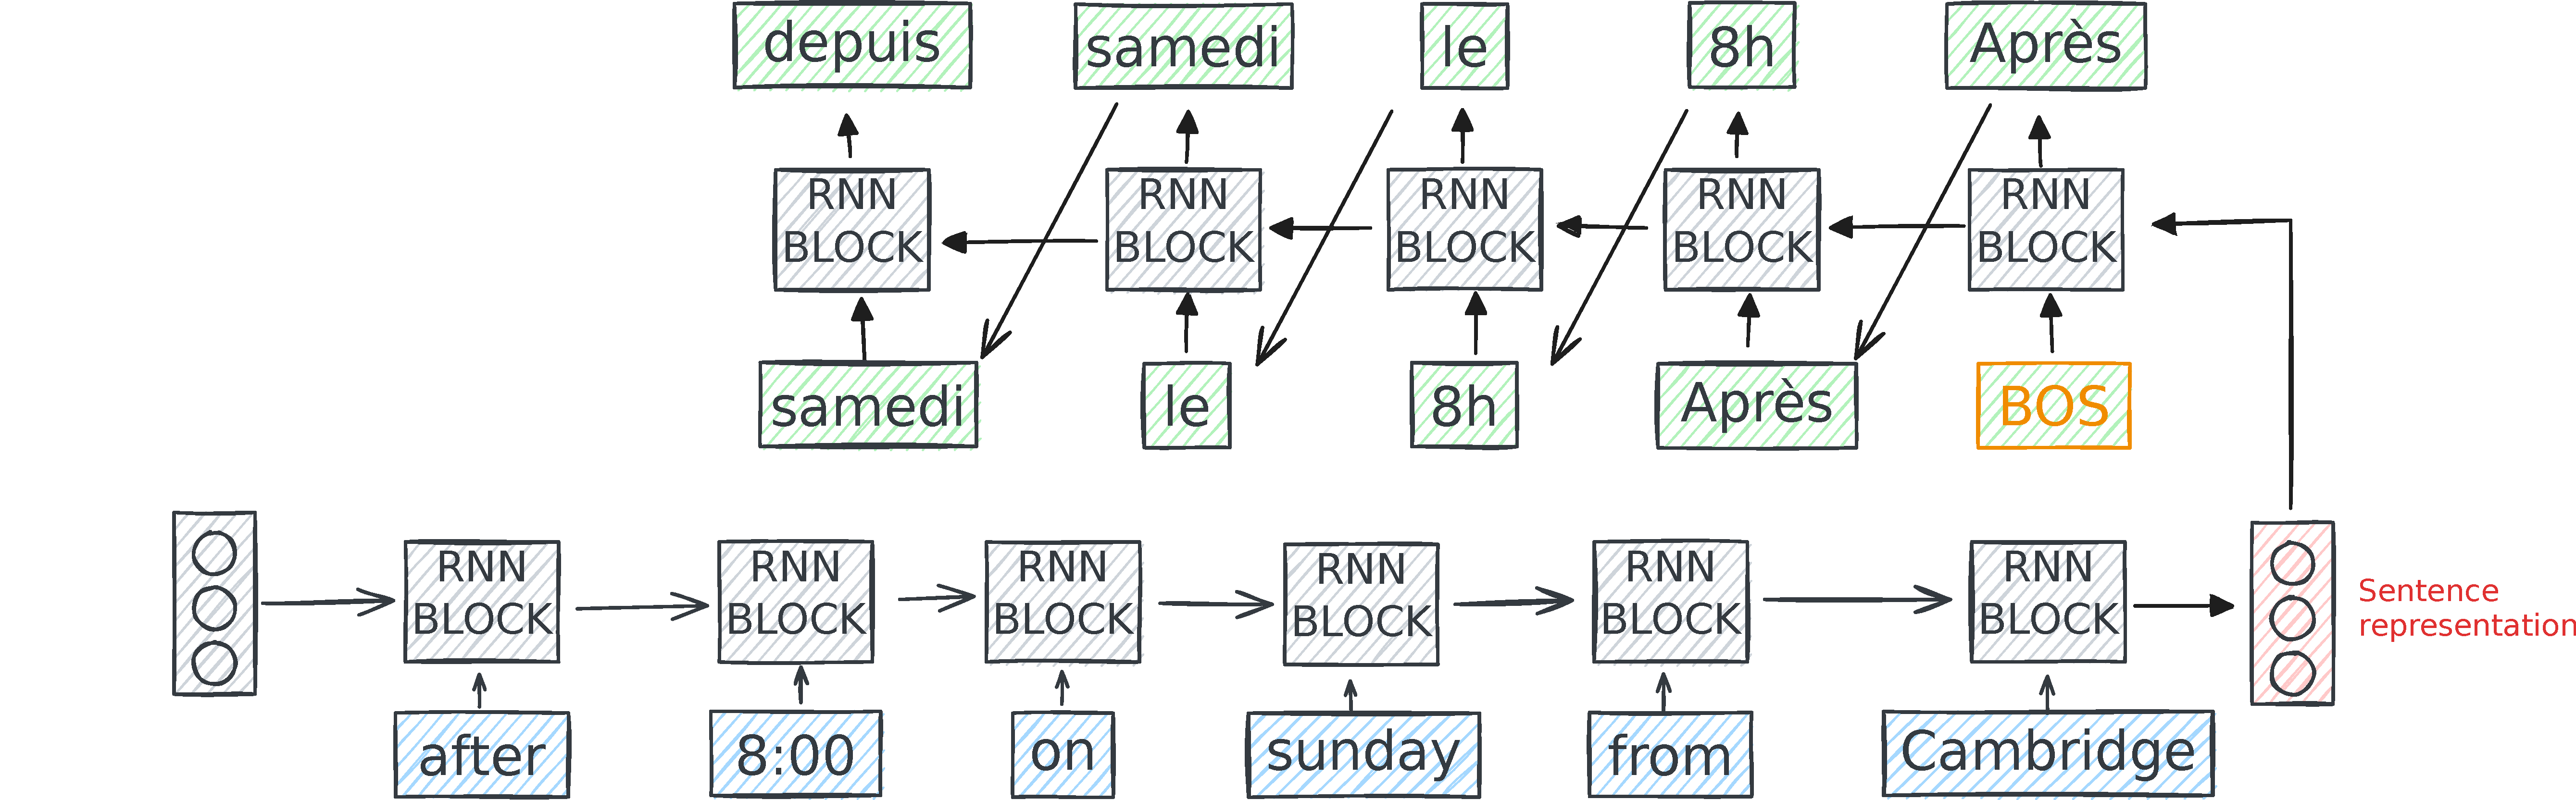
\includegraphics[width=1.\textwidth]{img/RNN-example-seq2seq-2.pdf}
    \end{figure}

    \phantom{\tiny \textbf{NB:} The \textit{EOS} word is a special word indicating the end of the sentence}

  \end{frame}

  \begin{frame}[noframenumbering]{Contextualize word in sentence: Seq2Seq with RNN}

    \begin{block}{Sequence to Sequence}
      \vspace{.1cm}
      {\footnotesize
        Model a sequence to sequence task with RNN :\\ 
        $\rightarrow $ Use \textit{``many to one''} variant to encode the input sequence\\
        $\rightarrow $ Use \textit{``one to many''} variant to generate a new sequence\\
      } 
    \end{block}

    \begin{figure}
      \centering
      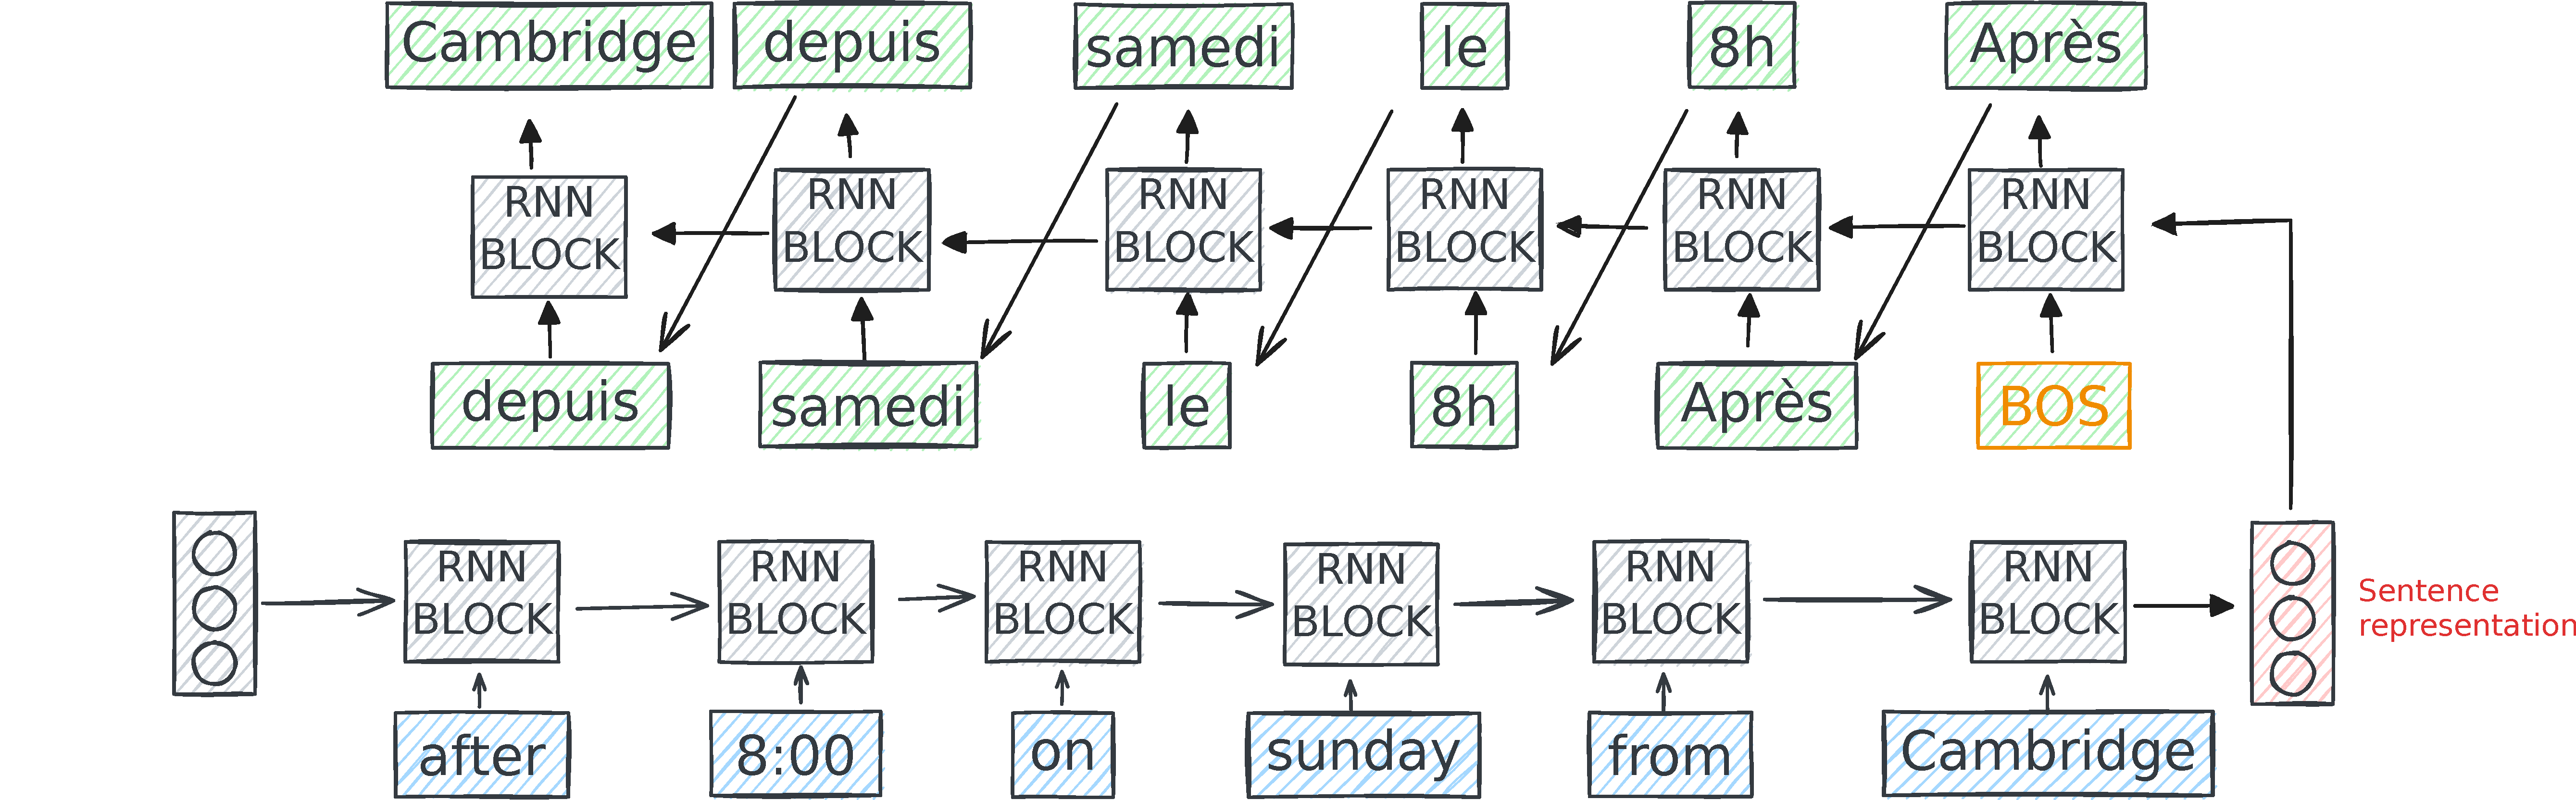
\includegraphics[width=1.\textwidth]{img/RNN-example-seq2seq-1.pdf}
    \end{figure}

    \phantom{\tiny \textbf{NB:} The \textit{EOS} word is a special word indicating the end of the sentence}
  \end{frame}


  \begin{frame}[noframenumbering]{Contextualize word in sentence: Seq2Seq with RNN}

    \begin{block}{Sequence to Sequence}
      \vspace{.1cm}
      {\footnotesize
        Model a sequence to sequence task with RNN :\\ 
        $\rightarrow $ Use \textit{``many to one''} variant to encode the input sequence\\
        $\rightarrow $ Use \textit{``one to many''} variant to generate a new sequence\\
      } 
    \end{block}

    \begin{figure}
      \centering
      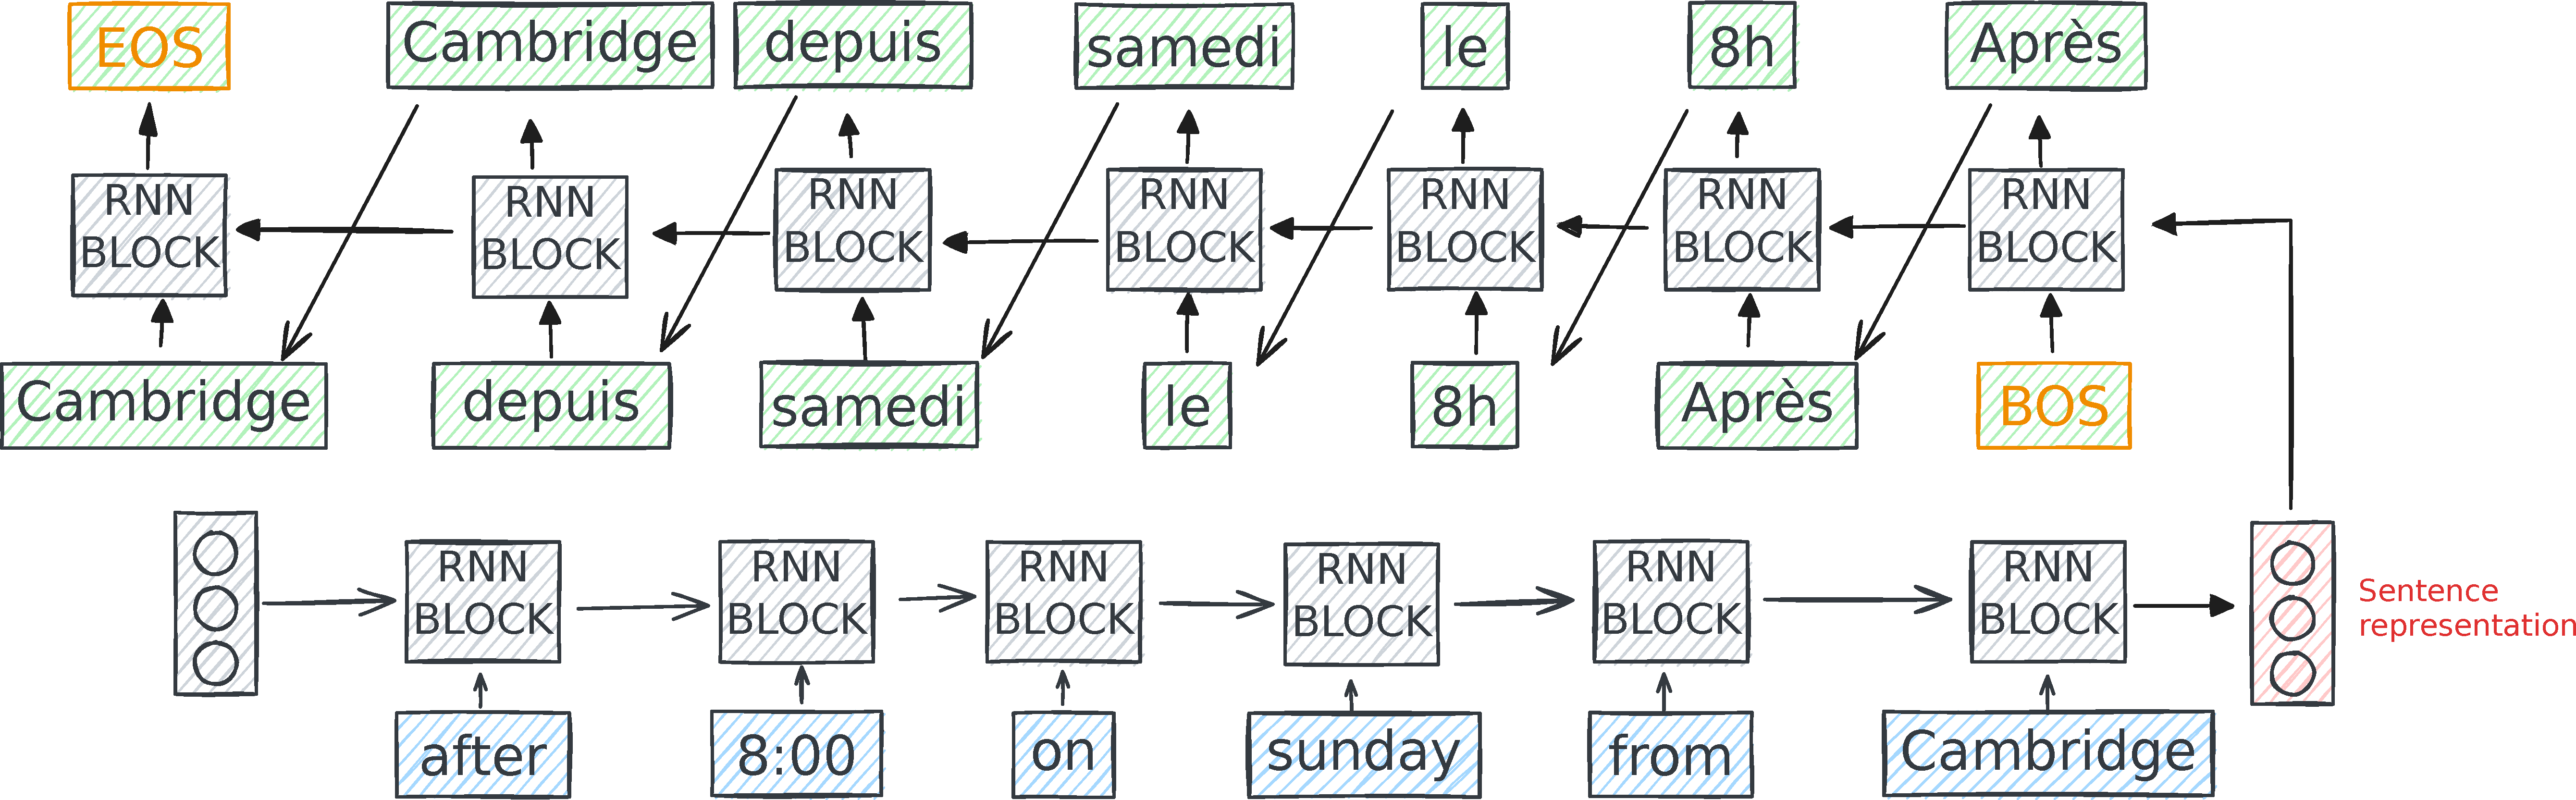
\includegraphics[width=1.\textwidth]{img/RNN-example-seq2seq-0.pdf}
    \end{figure}
    \pause
    {\tiny \textbf{NB:} The \texttt{EOS} word is a special word indicating the End Of the Sentence}
  \end{frame}


\begin{frame}{Exemple of ChitChat Bots}

            \begin{block}{Recurrent generative approach:}
                Essentially it is about learning to generate a sentence based on a given input sentence (and its context) \cite{serban-2016-building}
            \end{block}

    \begin{figure}
        \centering
        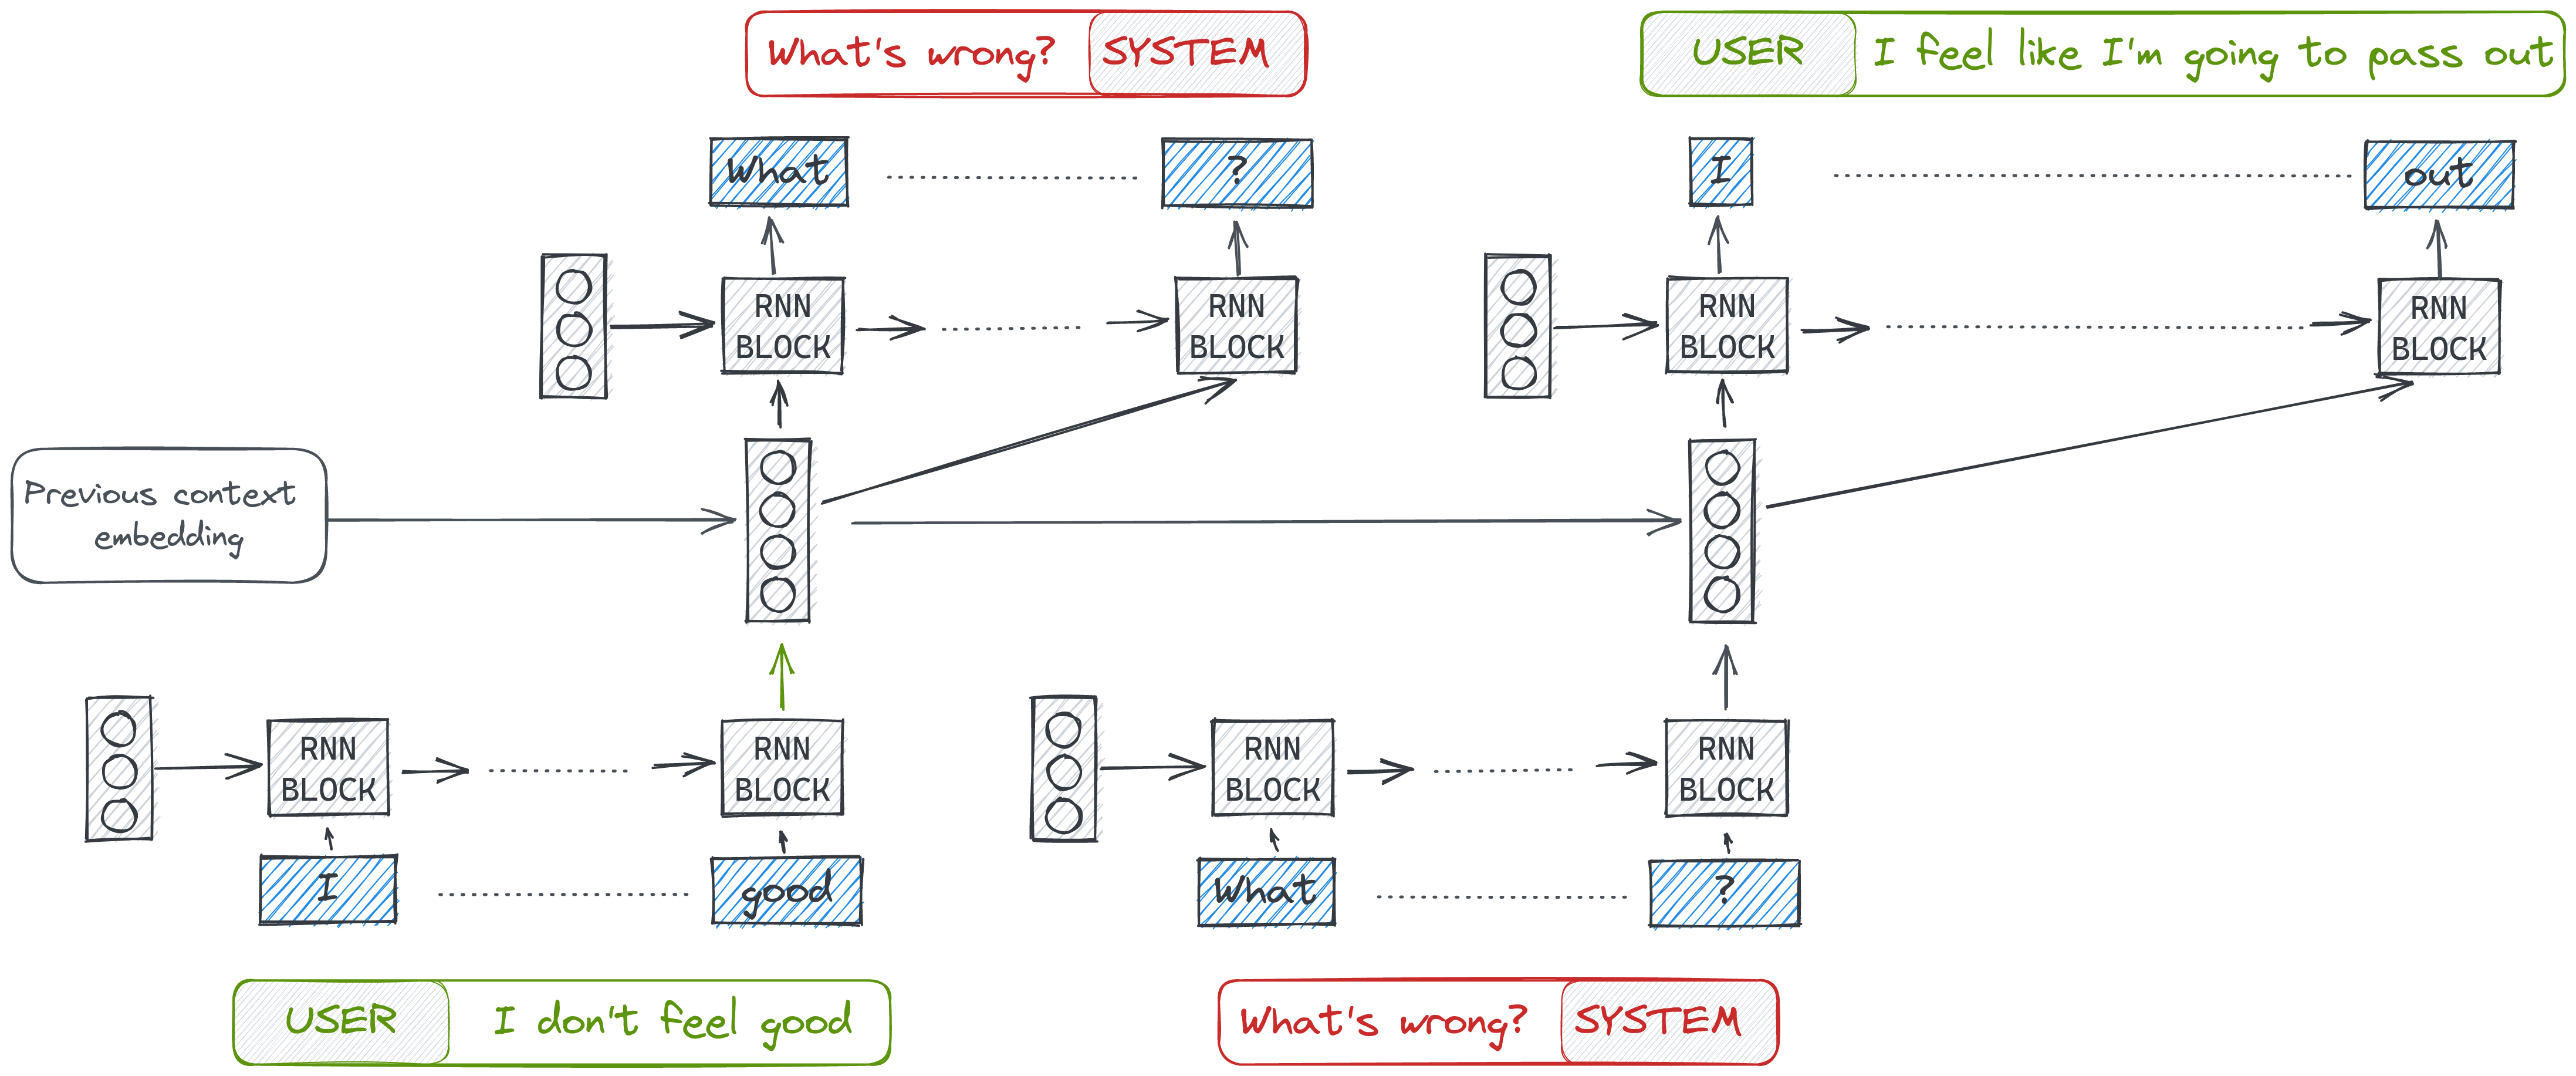
\includegraphics[width=.8\textwidth]{media/chitchat.png}
    \end{figure}
\end{frame}

\begin{frame}{Generative approaches for Task oriented systems}
    \textbf{Using generative approaches for dialogue systems ?}\\
    $\rightarrow$ Feeding the generator with context 

    \begin{figure}
        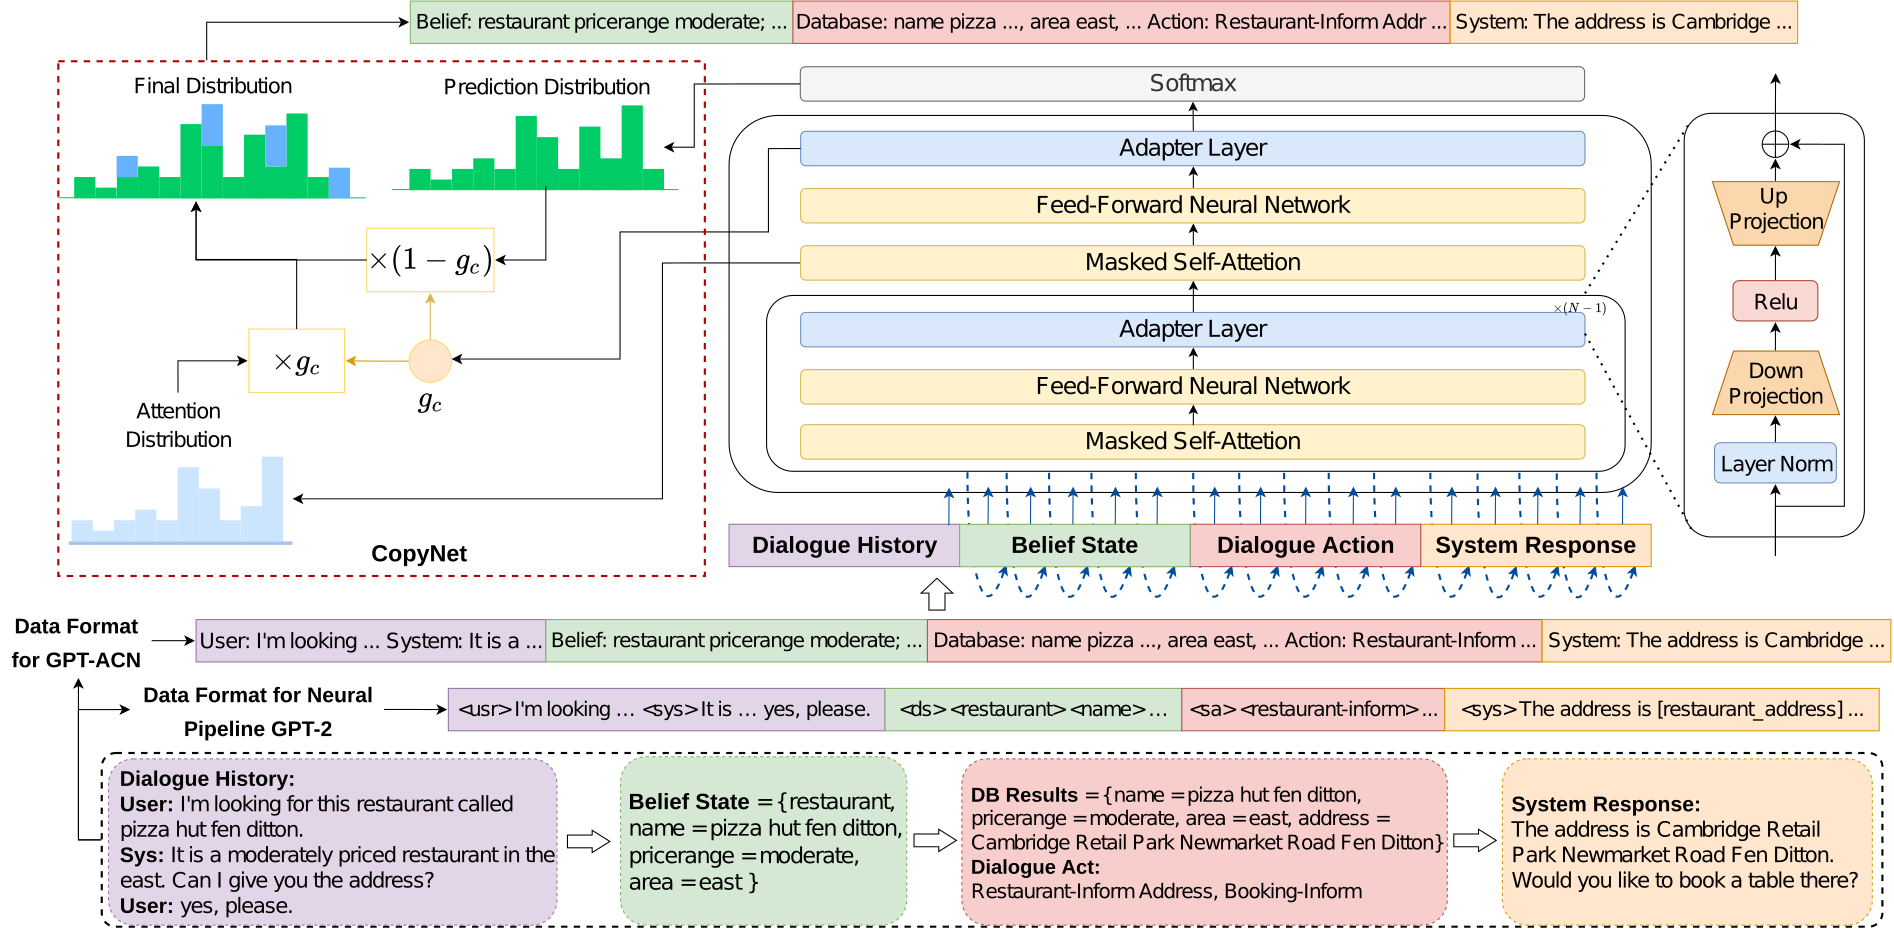
\includegraphics[width=1.\textwidth]{media/fully_generative.png}
    \end{figure}
\end{frame}

% \begin{frame}
%     \begin{columns}
%         \begin{column}{0.5\textwidth}
%             \begin{block}{Transformer approaches:}
%                 \cite{}
%             \end{block}

%         \end{column}
%         \begin{column}{0.5\textwidth}
%             \begin{figure}
%                 \centering
%                 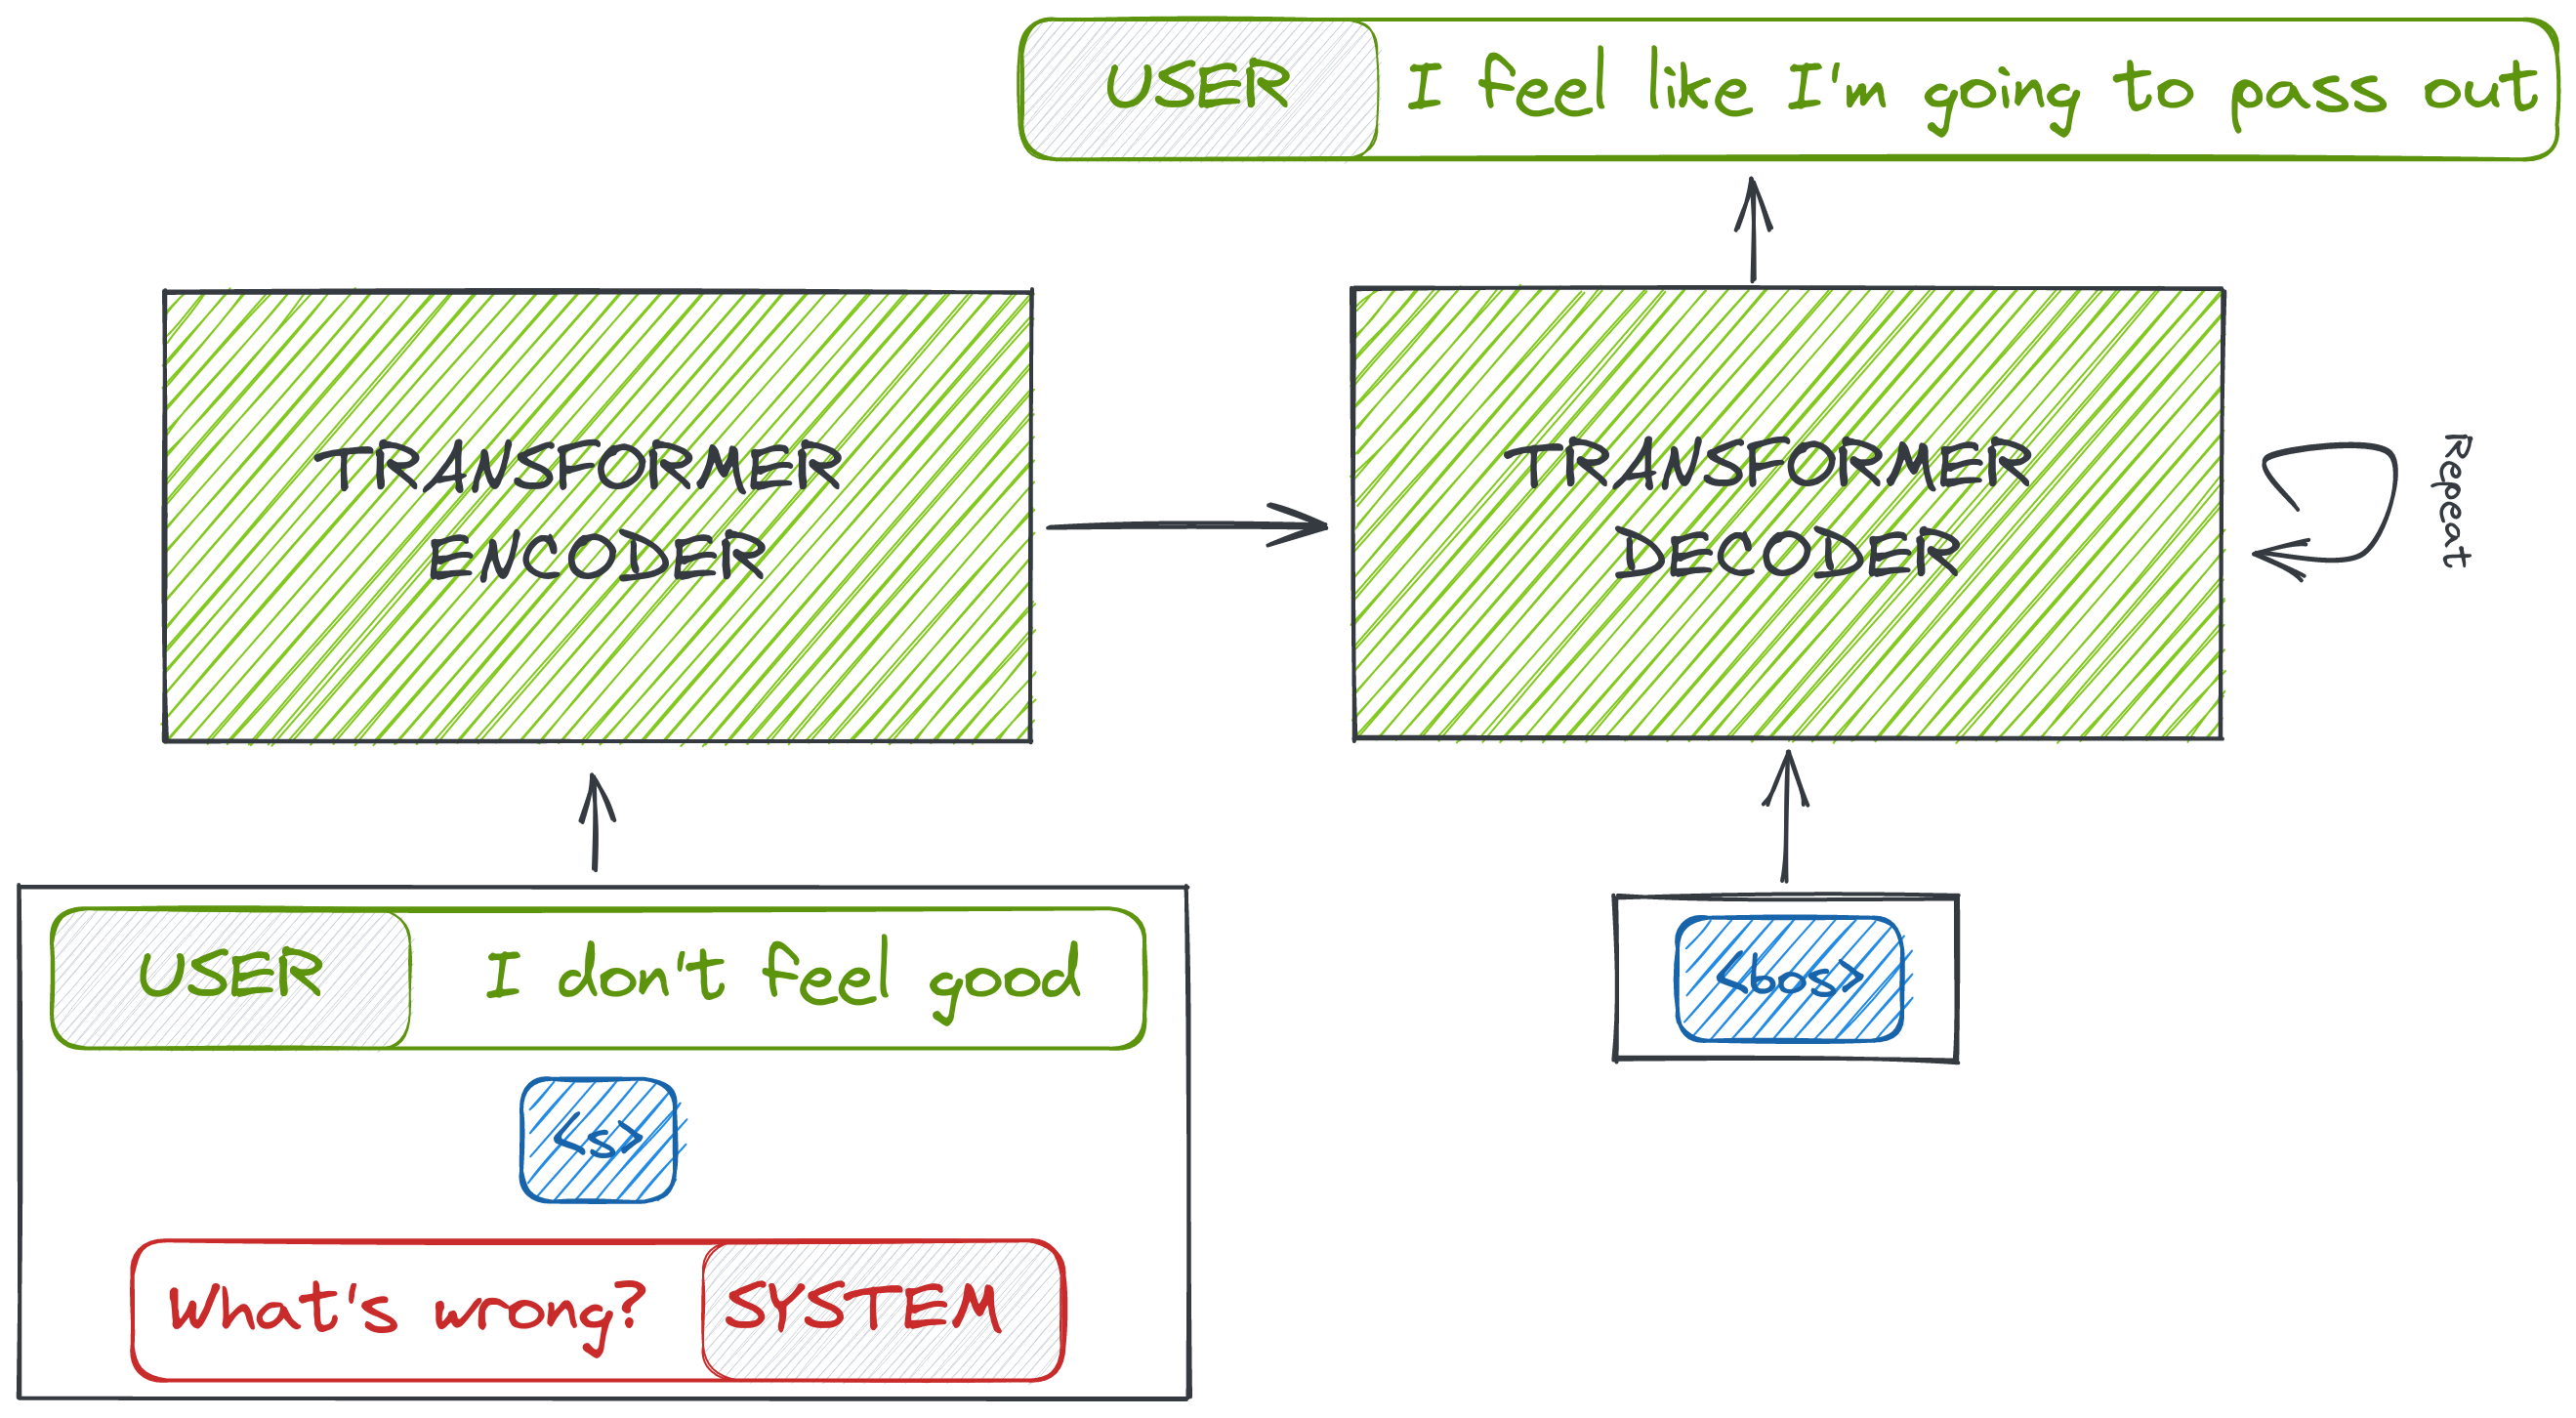
\includegraphics[width=1.\textwidth]{media/chitchat_transformer.png}
%             \end{figure}
%         \end{column}
%     \end{columns}

% \end{frame}

\section{Information Retrieval \& Question Answering}
\begin{frame}{Information Retrieval systems}
    \begin{columns}
        \begin{column}{0.5\textwidth}
             \begin{block}{Conversationnal Information retrieval systems}
                \begin{itemize}
                    \item The answers are documents (or answer are based on summarizing document information)
                    \item The objective is to retrieve documents within answer to user utterance is in
                \end{itemize}
            \end{block}       
        \end{column}
        \begin{column}{0.5\textwidth}
            \begin{figure}
                \centering
                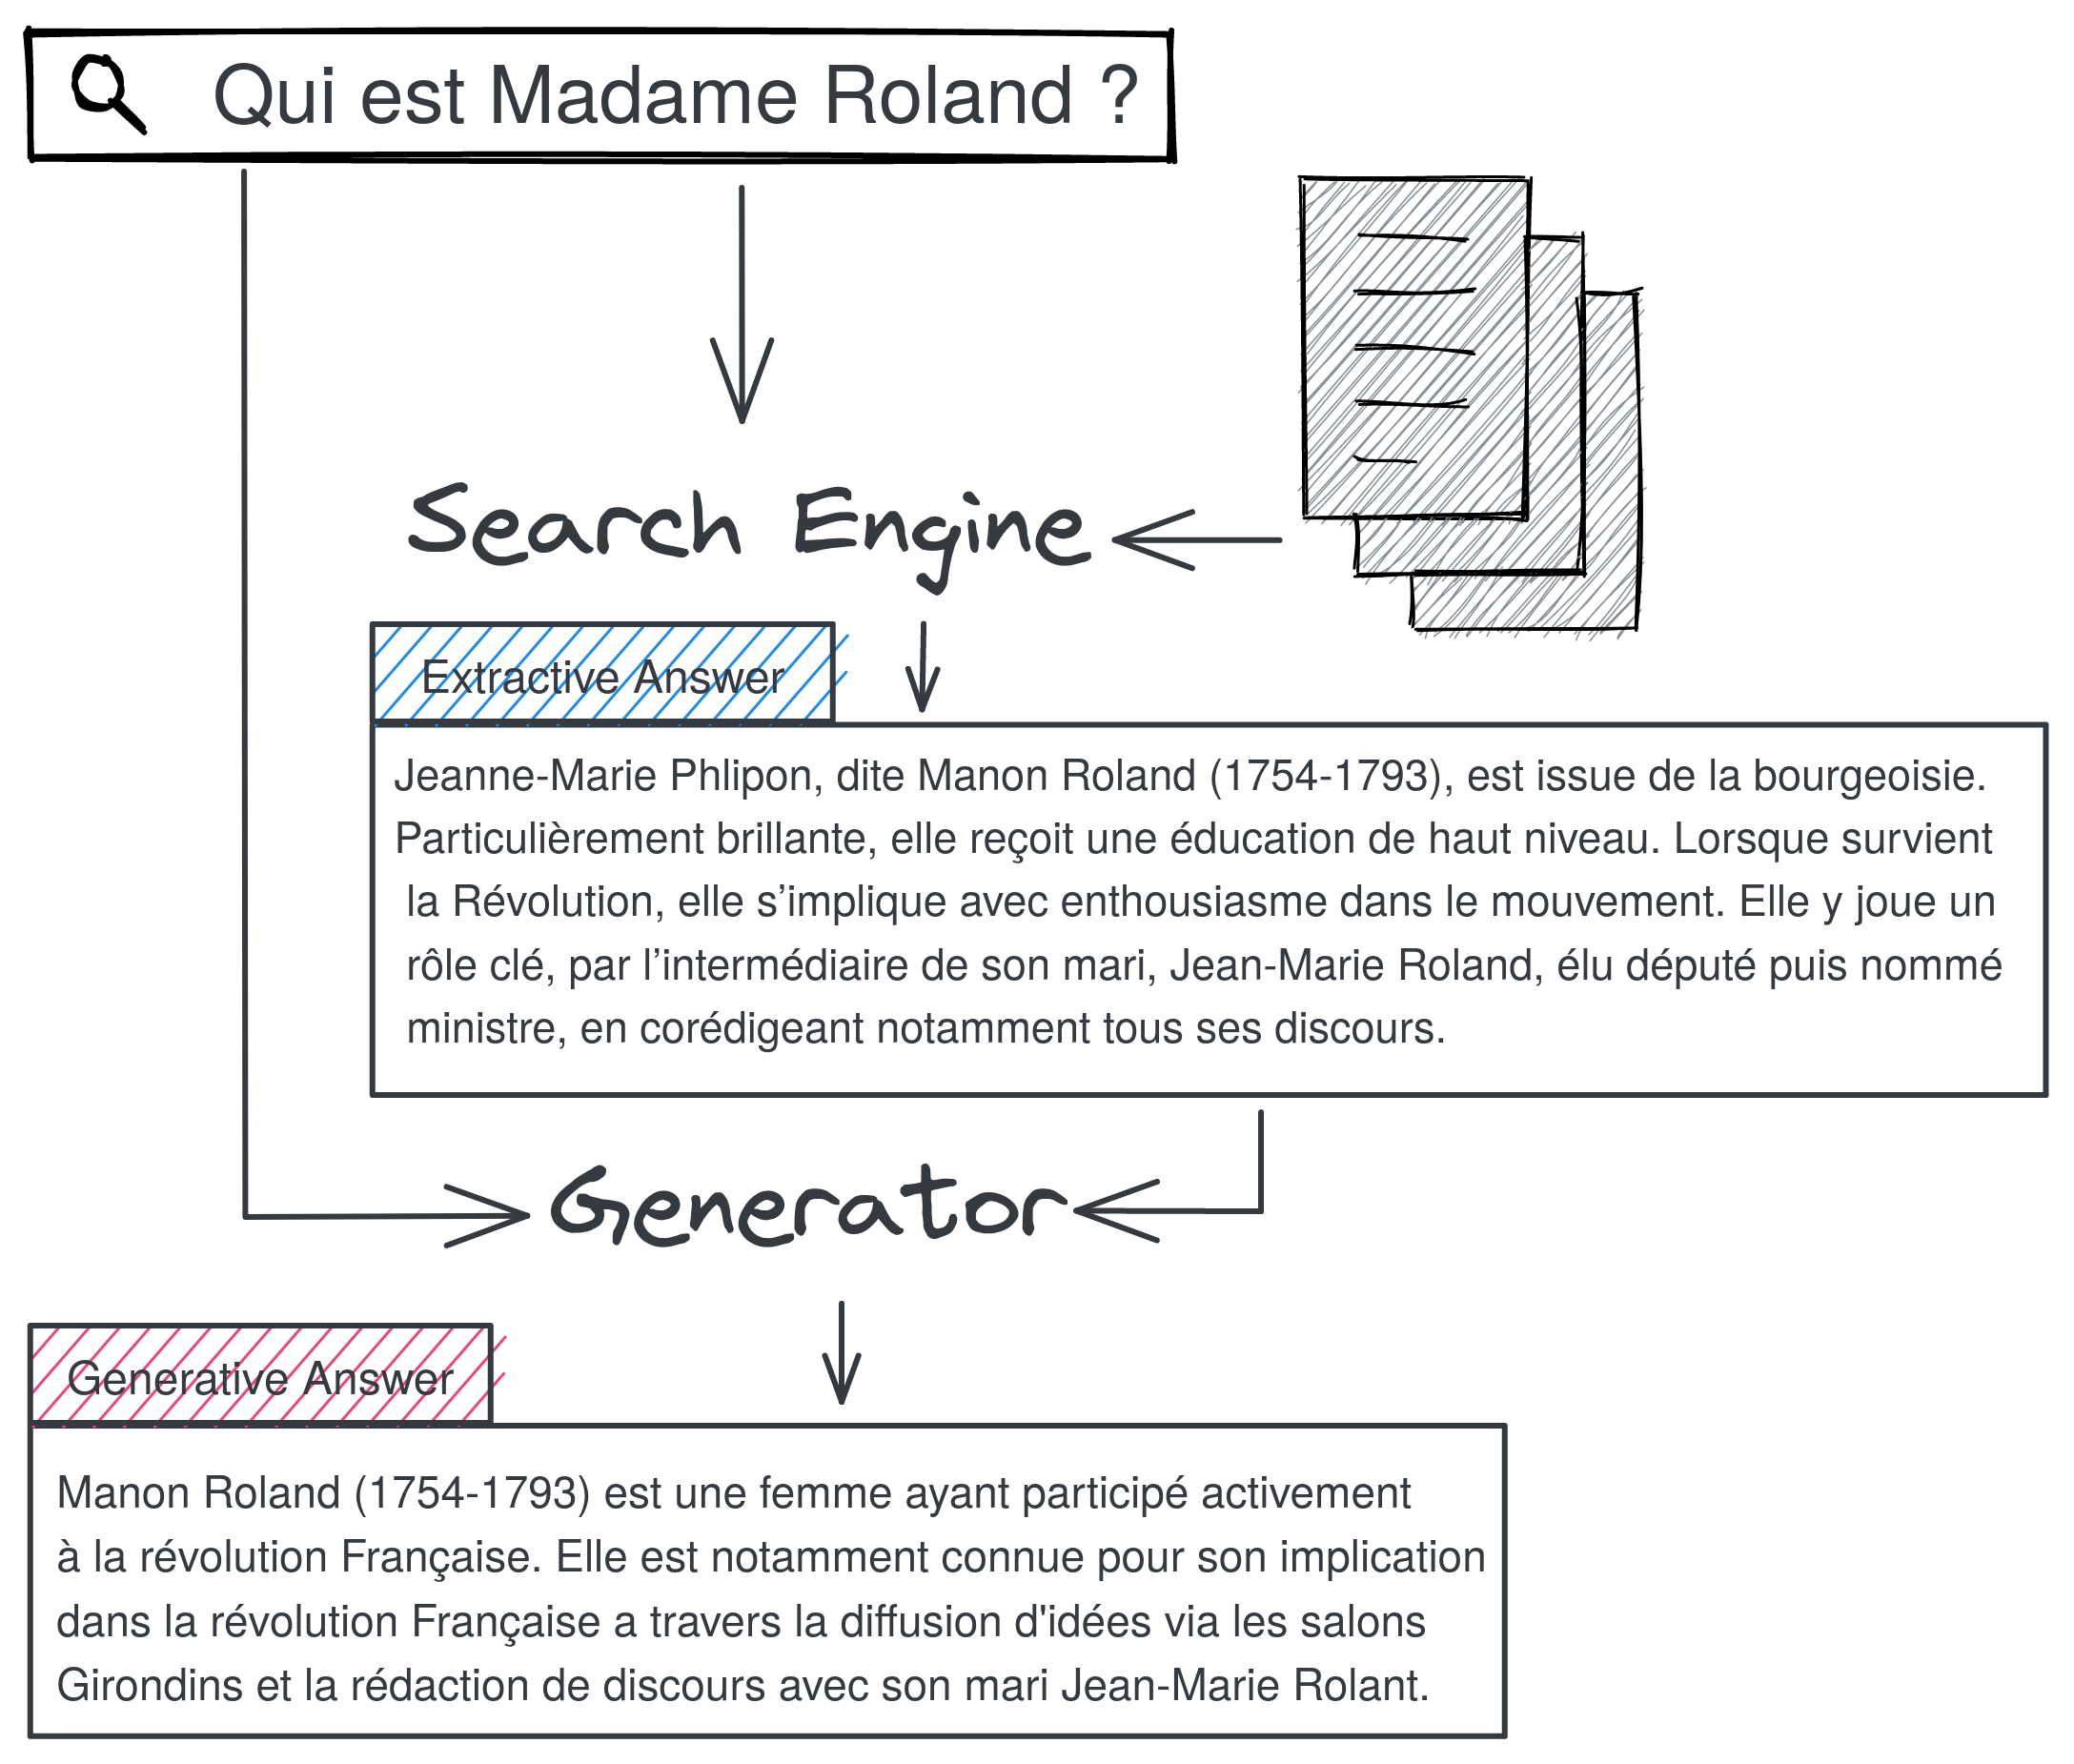
\includegraphics[width=.9\textwidth]{media/who-is-rolland.png}
                \caption{\scriptsize A QA model based on documents search : firstly extract and then rephrase to produce an answer allow to better source/verify information.}
                \label{fig:my_label}
            \end{figure}
        \end{column}
    \end{columns}
\end{frame}

\begin{frame}{Information Retrieval}
    \begin{columns}
        \begin{column}{0.5\textwidth}
               \begin{block}{How to search}
            \begin{itemize}
                \item Word/word frequency based search (Bow/tf-idf/BM25)
                \item Neural Networks (Learning to rank, Transformer based approaches)
            \end{itemize}
        \end{block}
        \begin{block}{In a conversation}
            \begin{itemize}
                \item Request depends on previous utterance (answer and question)
                \item Query with no context in the current utterances
            \end{itemize}  
        \end{block} 
        \end{column}
        \begin{column}{0.5\textwidth}
            \begin{block}{Approaches}
                \begin{itemize}
                    \item Entity linking
                    \item Query reformulation (with history)
                    \item Ranking on history (end2end) \cite{nam-2023-cosplade}
                    \item Ranking and select answer using history selection (or whole history) \cite{Qu_2019}%wizard of wikipedia
                \end{itemize}
            \end{block}
            Take a look at the TREC CASt competition
        \end{column}
    \end{columns}

\end{frame}


\begin{frame}{Question answering}
    \begin{columns}
        \begin{column}{0.5\textwidth}
            \begin{block}{QA: different approaches}
                \begin{itemize}
                    \item Retirieved documents/Knowledge triplets retrieved (RI)
                    \item Information is ``stored/compressed'' in the model weights (GPT like)
                    \item Within context (text is given as input of the model)
                \end{itemize}
            \end{block}
        \end{column}
        \begin{column}{0.5\textwidth}   
            \begin{block}{Some dataset}
                \begin{itemize}
                    \item Non conversational 
                        \begin{itemize}
                            \item SQuAD (FQuAD)
                            \item Natural Question
                            \item HotpotQA
                        \end{itemize}
                    \item Conversational 
                        \begin{itemize}
                            \item QuAC 
                            \item CoQA
                        \end{itemize}
                \end{itemize}
            \end{block}
        \end{column}
    \end{columns}
\end{frame}




\begin{frame}{Task Oriented Systems :  Evaluate NLU/State/DA}
    \begin{block}{NLU/State/DA evaluation:}
        Does retrieved domain, intents and slots type/values correspond to what is expected ?
        \begin{itemize}
             \item \textbf{Domain, Intent} Multiclass classification (mono-label) : \\
            $$accuracy = \frac{# correctly\ predicted}{# number\ of\ predictions}$$
            \item \textbf{slot type/values} Multiclass classification (multi-label) 
                \begin{itemize}
                    \item \textbf{precision/recall} $$precision=\frac{TP}{TP+ FP}$$ $$recall=\frac{TP}{TP + FN}$$
                    \item \textbf{F1-score}  $$F1 = 2\frac{precision\times recall}{precision + recall}$$
                    
                \end{itemize}
                for non categorical slot value use exact match? /use partial match?
        \end{itemize}    
    \end{block}
\end{frame}


\begin{frame}{Evaluate Generated text}
    \begin{block}{Comparing the ground truth to generated text}
        
    \end{block}
    
\end{frame}
\begin{frame}{Evaluate Generation}
    \begin{columns}
        \begin{column}{0.6\textwidth}
            \begin{block}{Automatic evaluation}
                Evaluating simalirity with the ground truth :
                \begin{itemize}
                    \item \textbf{On tokens/words level: } Counting the number of similar words or ``N-grams'' (e.g BLEU, ROUGE, METEOR)
    
                    \item \textbf{On embeddings level} : Embed text and compare embeddings (may takes into account synonyms) such as the BERTScore\cite{}
                    \item \textbf{Entity} (between ground truth and generation)
                \end{itemize}
                
            \end{block}     
        \end{column}
        \begin{column}{0.4\textwidth}
            \begin{block}{Human evaluation}
                An example of evaluations approaches \cite{Thorleiksdttir2021UnderstandingHPb}
                \begin{itemize}
                    \item Fluency 
                    \item adequacy/informativness
                    \item grammatical correctness
                \end{itemize}
                
            \end{block}
            
        \end{column}
    \end{columns}

\end{frame}

% \begin{frame}{End-to-end question answering generative process}
%     \begin{figure}
%         \centering
%         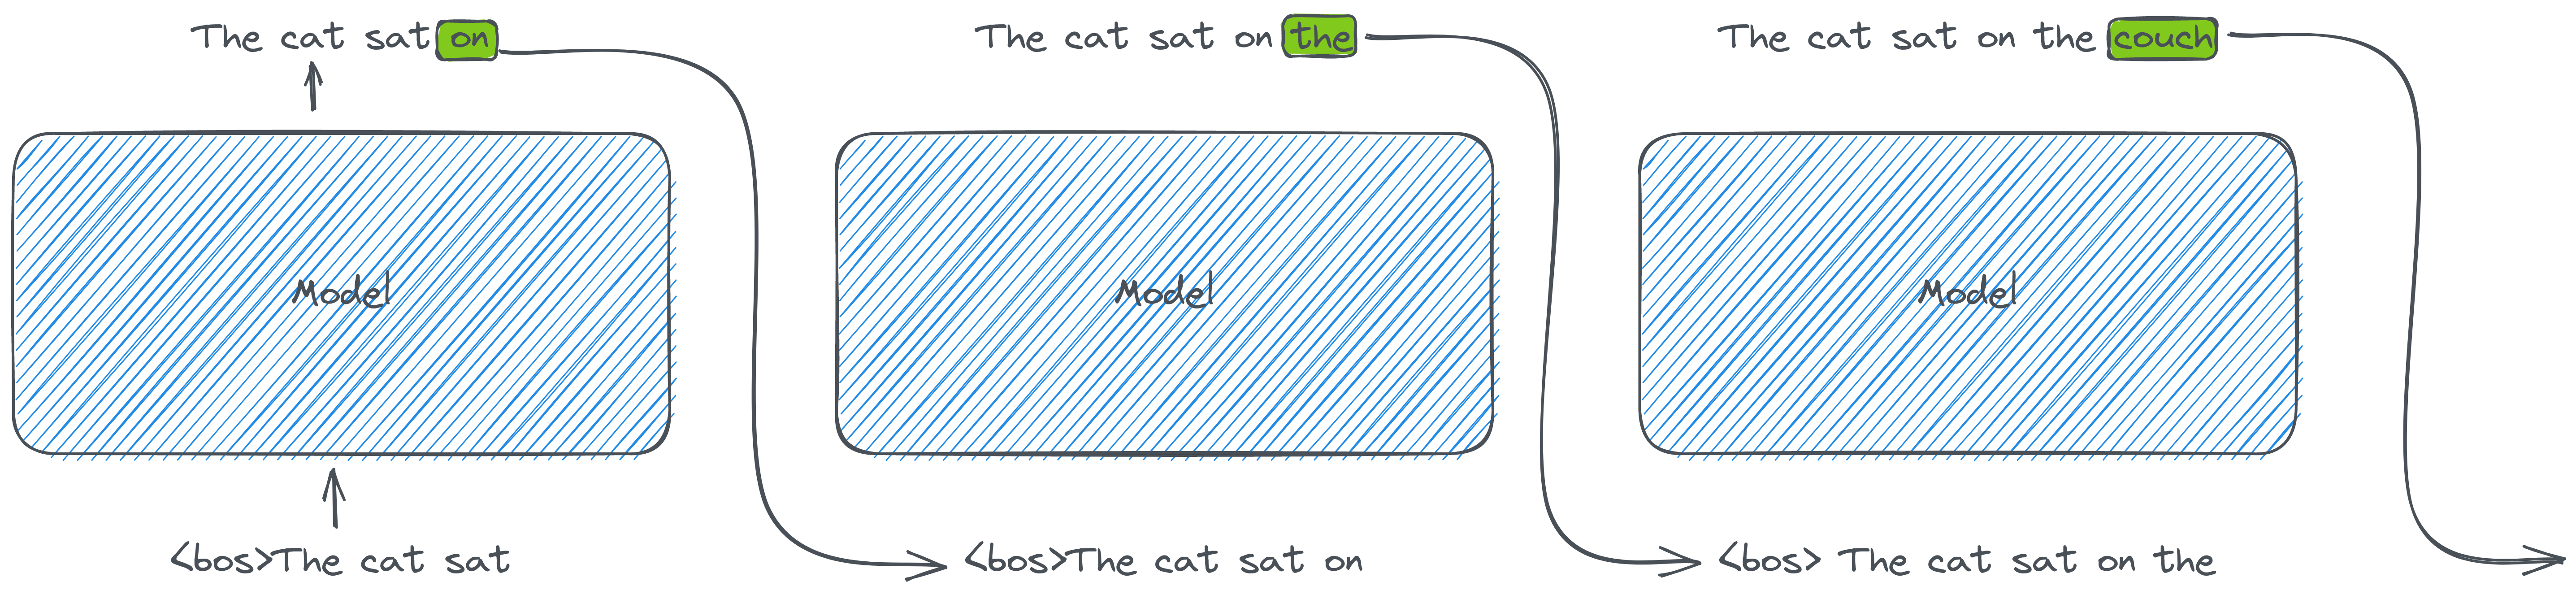
\includegraphics[width=0.99\textwidth]{media/text-generation.png}
%         \caption{Previous utterances can be stack previously inthe generative model}
%         \label{fig:my_label}
%     \end{figure}
% \end{frame}
\begin{frame}{End-to-end question answering (+chitchat) : ChatGPT}
    \begin{columns}
        \begin{column}{0.5\textwidth}
            \begin{alertblock}{GPT (Generative Pretrained Transformer) models}
                The GPTs model consider only a decoder part
                \begin{itemize}
                    \item GPT \footnotesize{(Improving language understanding by Generative Pre-Training, 2018)} \\
                        \textit{\scriptsize A Transformer fine-tuned on different task}
                    \item GPT-2 \footnotesize{(Language Models are Unsupervised Multitask Learners, 2019)} \\
                        \textit{\scriptsize A prompt model (tasks is only based on natural language or using instruction)}
                    \item GPT-3 \footnotesize{(Language Models are Few-Shot Learners, 2020)} \\
                        \textit{\scriptsize 175 billion parameters}
                    \item ChatGPT/Instruct-GPT \footnotesize{(Training language models to follow instructions, 2022)} \\
                        \textit{\scriptsize GPT-3/3.5 ``fine-tuned'' using reinforcement learning} 
                \end{itemize} 
            \end{alertblock}
        \end{column}
        \begin{column}{0.5\textwidth}
            \begin{figure}
                \centering
                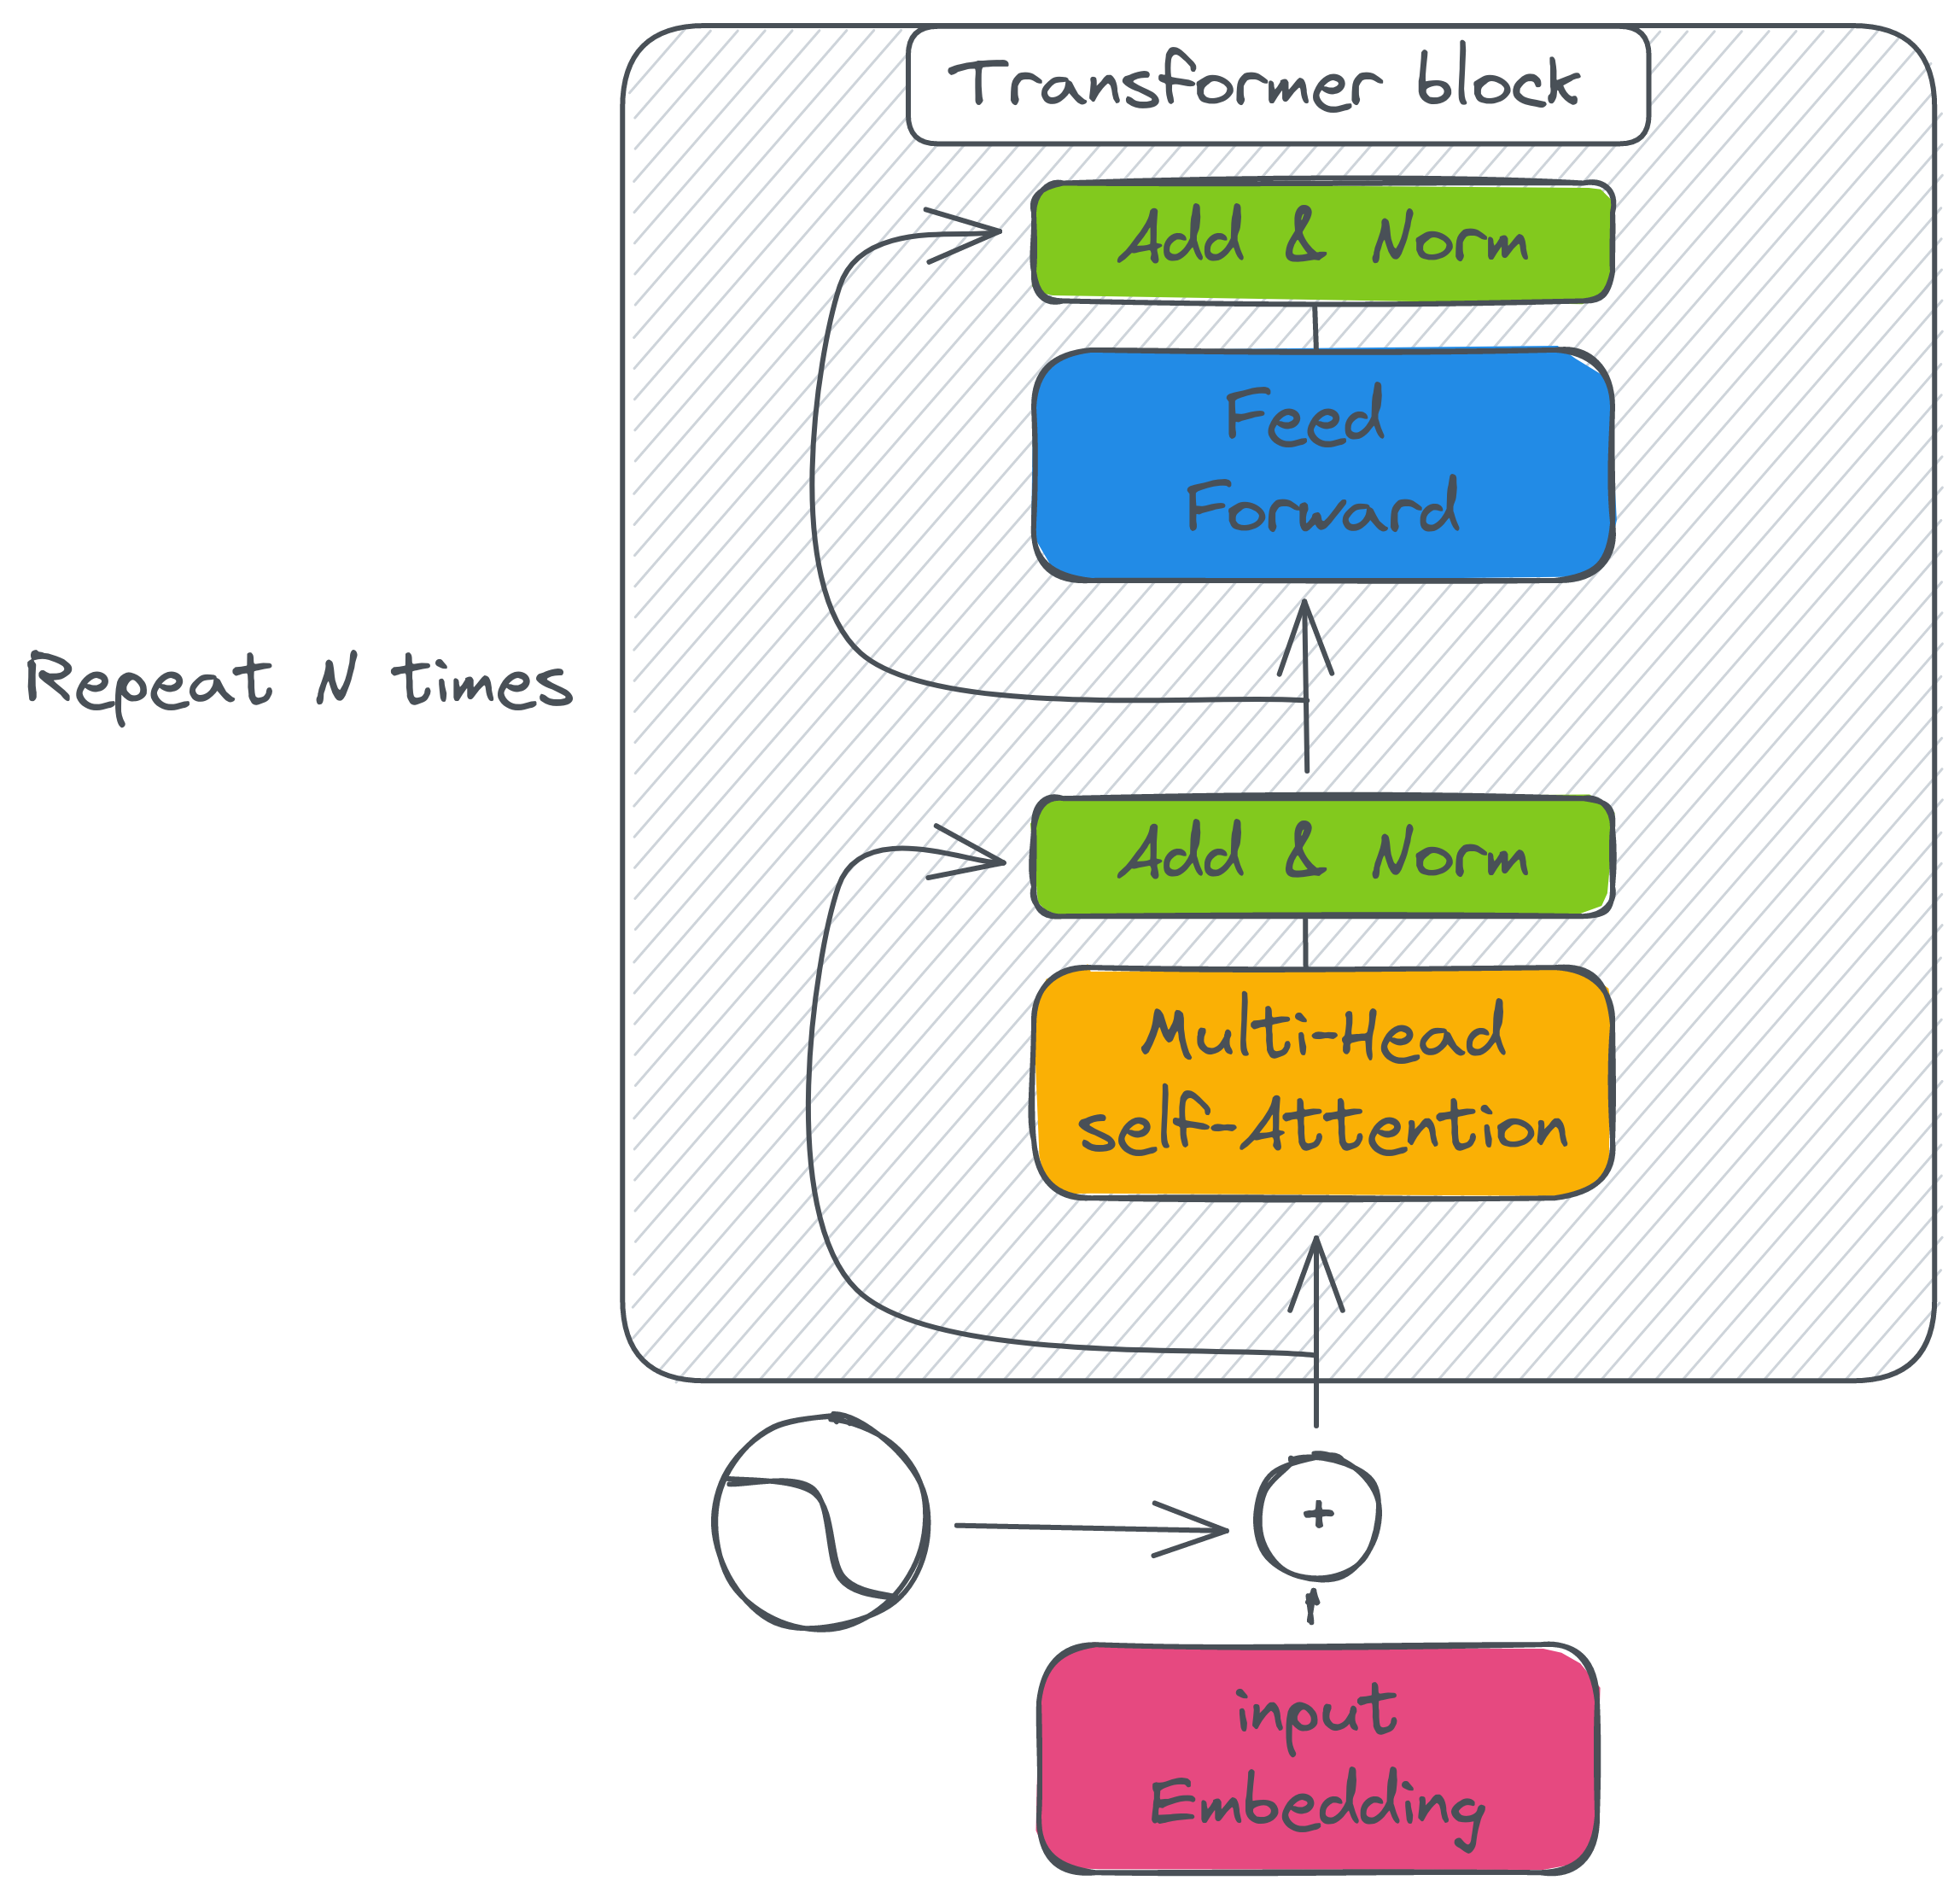
\includegraphics[width=.9\textwidth]{media/transformer-block.png}
                \caption{GPTs models are only based on the decoder part of the transformer architecture}
                \label{fig:my_label}
            \end{figure}
        \end{column}
    \end{columns}
\end{frame}
\begin{frame}{Instruct GPT: What you need is data}

    \begin{columns}
        \begin{column}{0.5\textwidth}
            \begin{alertblock}{What make it works}
                \begin{itemize}
                    \item \textbf{Step-0 :} Accumulation of world knowledge (large model needed).
                    \item \textbf{Step-1 :}  Fine tuning on carefully selected data (13k for instruct gpt). It learns to follow instructions.
                    \item \textbf{Step-3 :} "Fine tune" the model  in order to maximise a score (given by a reward model) using reinforcement learning. One may interpret it as learning to generalize the \textbf{step 1} to unseen ``tasks''.
                \end{itemize}

            \end{alertblock}

        \end{column}
        \begin{column}{0.6\textwidth}  %%<--- here
            \begin{figure}
                \centering
                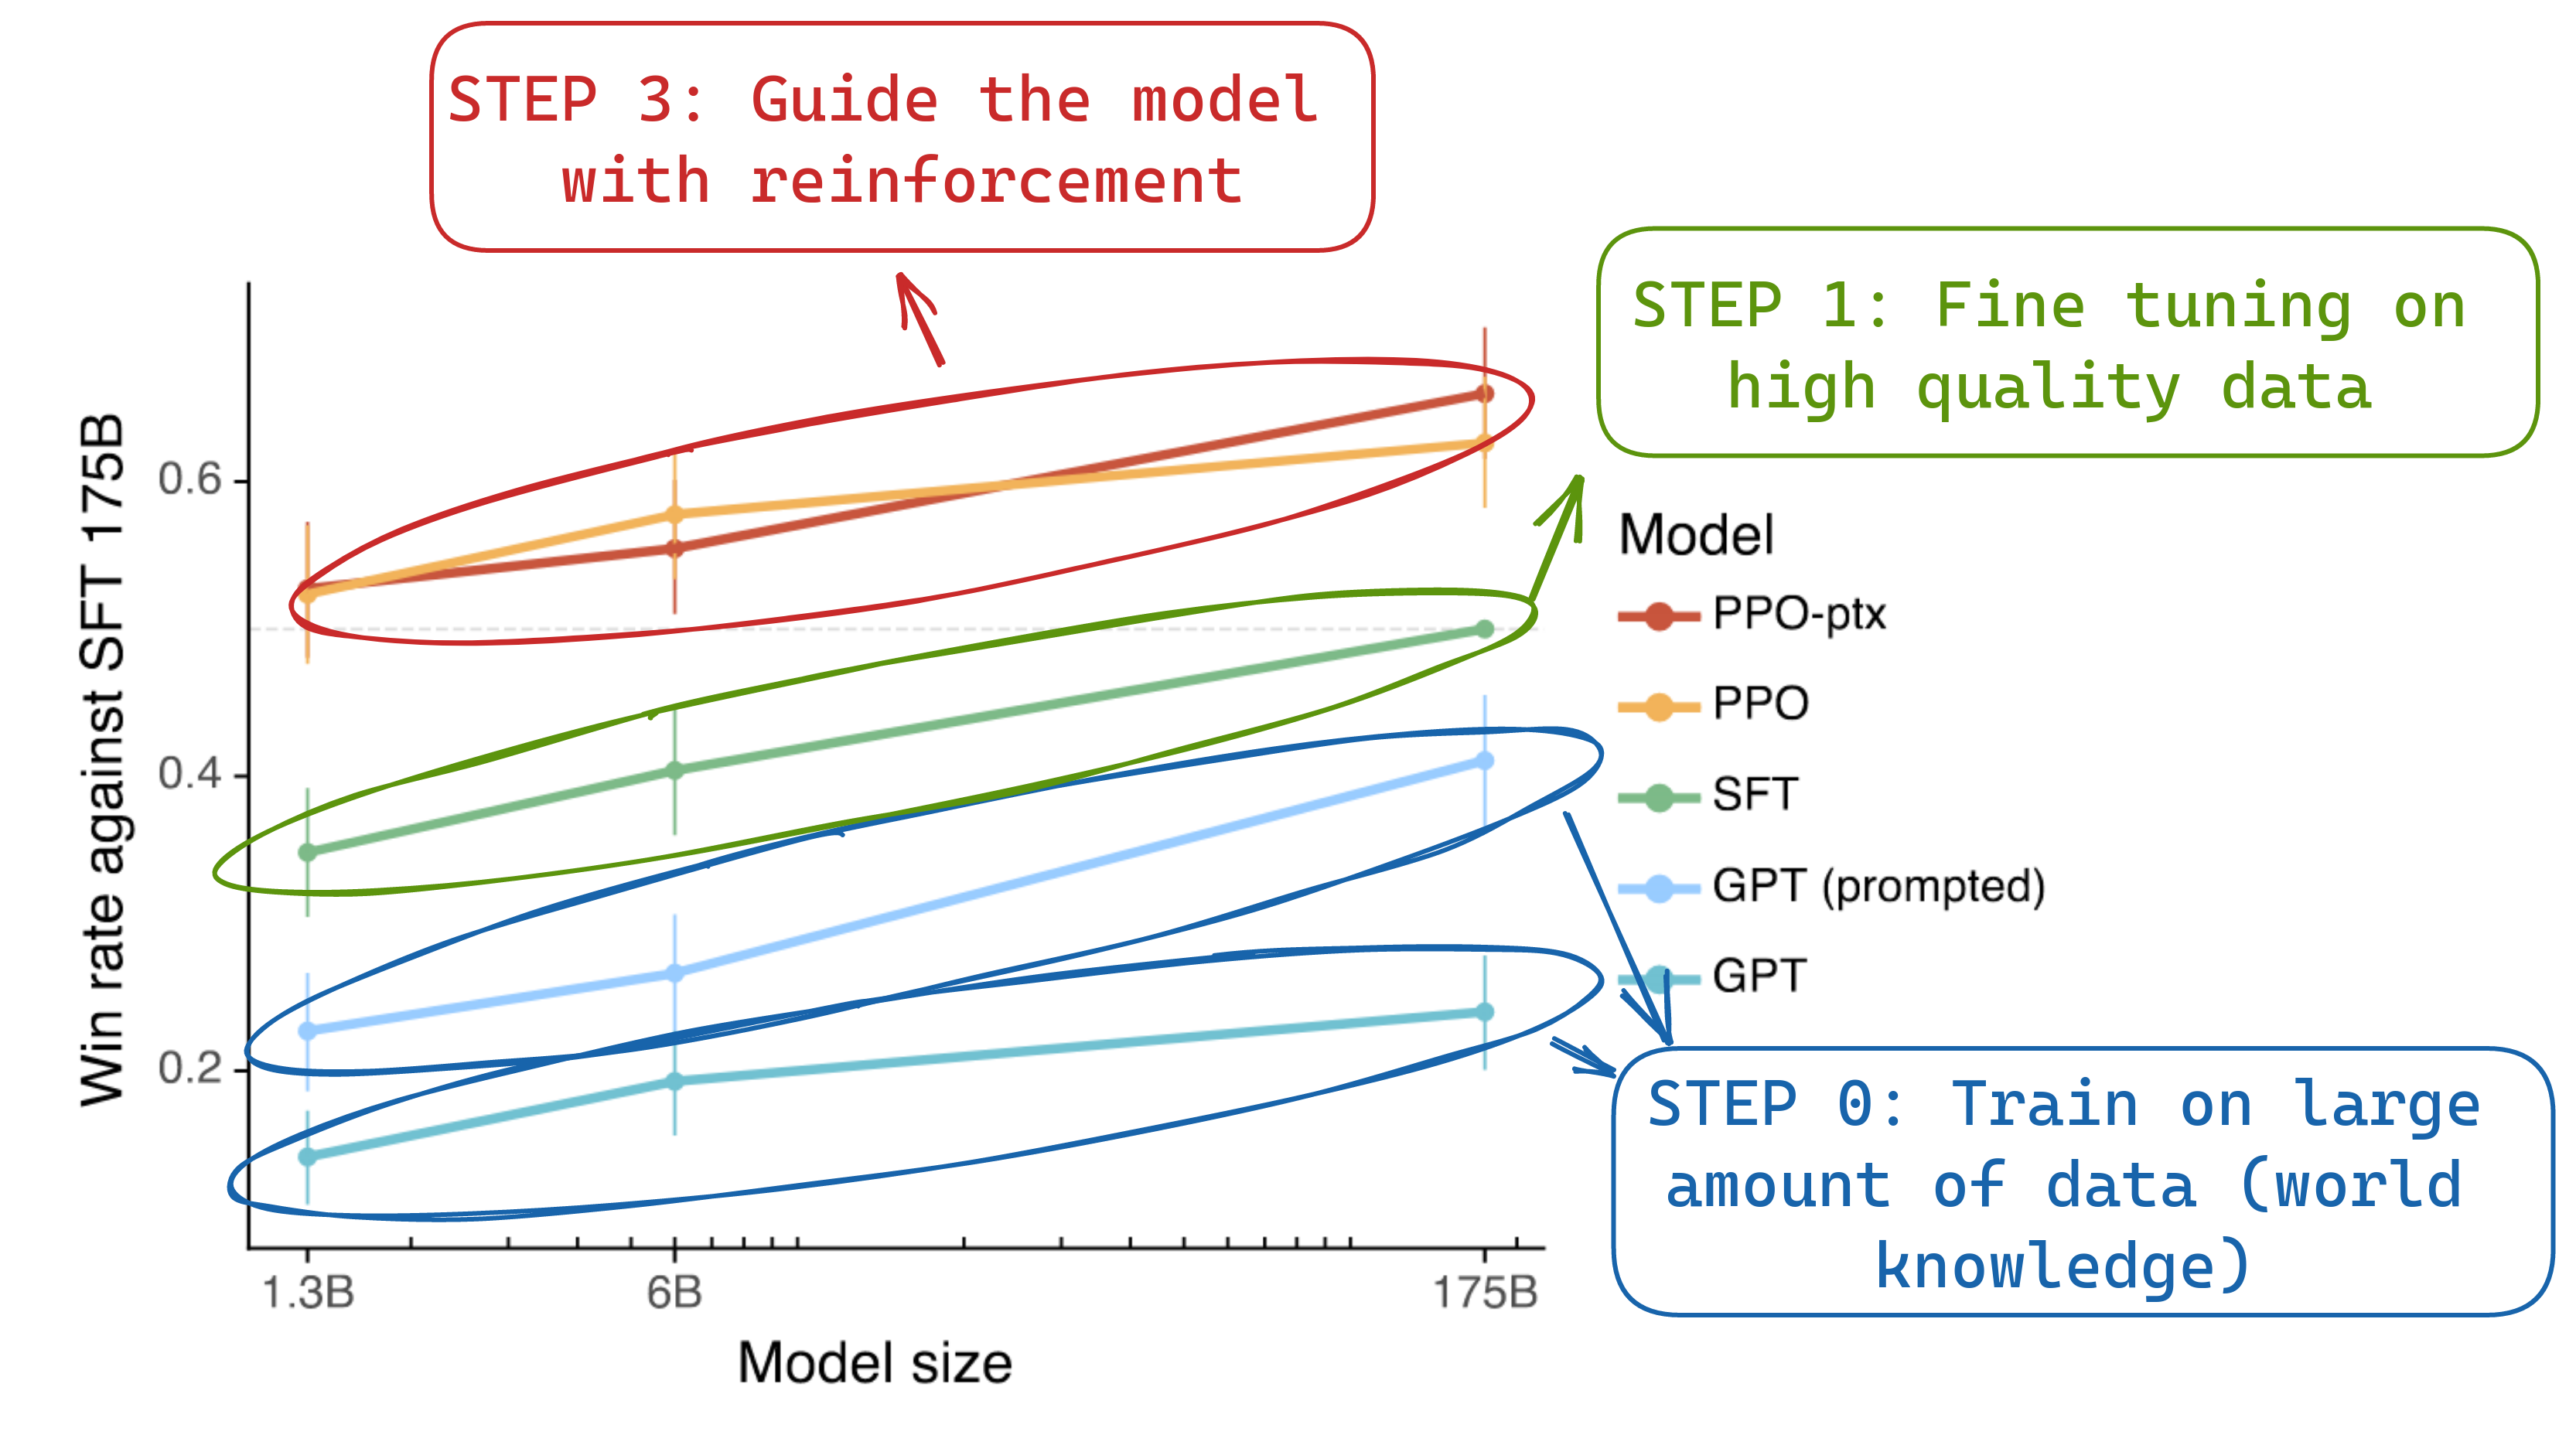
\includegraphics[width=1.\textwidth]{media/why-chatgpt.png}
                
                
            \end{figure}
        \end{column}
    \end{columns}
\end{frame}

\begin{frame}{Instruct GPT: Step 0 Gathering world knowledge}

    \begin{columns}
        \begin{column}{0.5\textwidth}
            \begin{table}[]
                \centering
                \footnotesize
                \begin{tabular}{l|c|p{2.8cm}}
                    Corpus & Tokens & Desc \\
                    \hline
                    Common Crawl & 410B &  Web page crawled \\
                    Books$_1$ & 19B & Collection of books \\
                    Books$_2$ & 12B & Collection of books \\
                    Wikipedia & 3B & Encyclopedic content
                \end{tabular}
                \caption{Sample of collections used to train base GPT-3 model. Some data are filtered or unseen during the training (particularly for \textit{Common Crawl} corpus}
                \label{tab:gpt3-corpus}
            \end{table}
            \begin{alertblock}{Training on a very large amount of data}
        
                \begin{itemize}
                    \item Gathering general knowledge
                    \item Structure of languages
                    \item Prompt based generation
                \end{itemize}

            \end{alertblock}

        \end{column}
        \begin{column}{0.5\textwidth}  %%<--- here
            \begin{alertblock}{}
        
                \begin{figure}
                    \centering
                    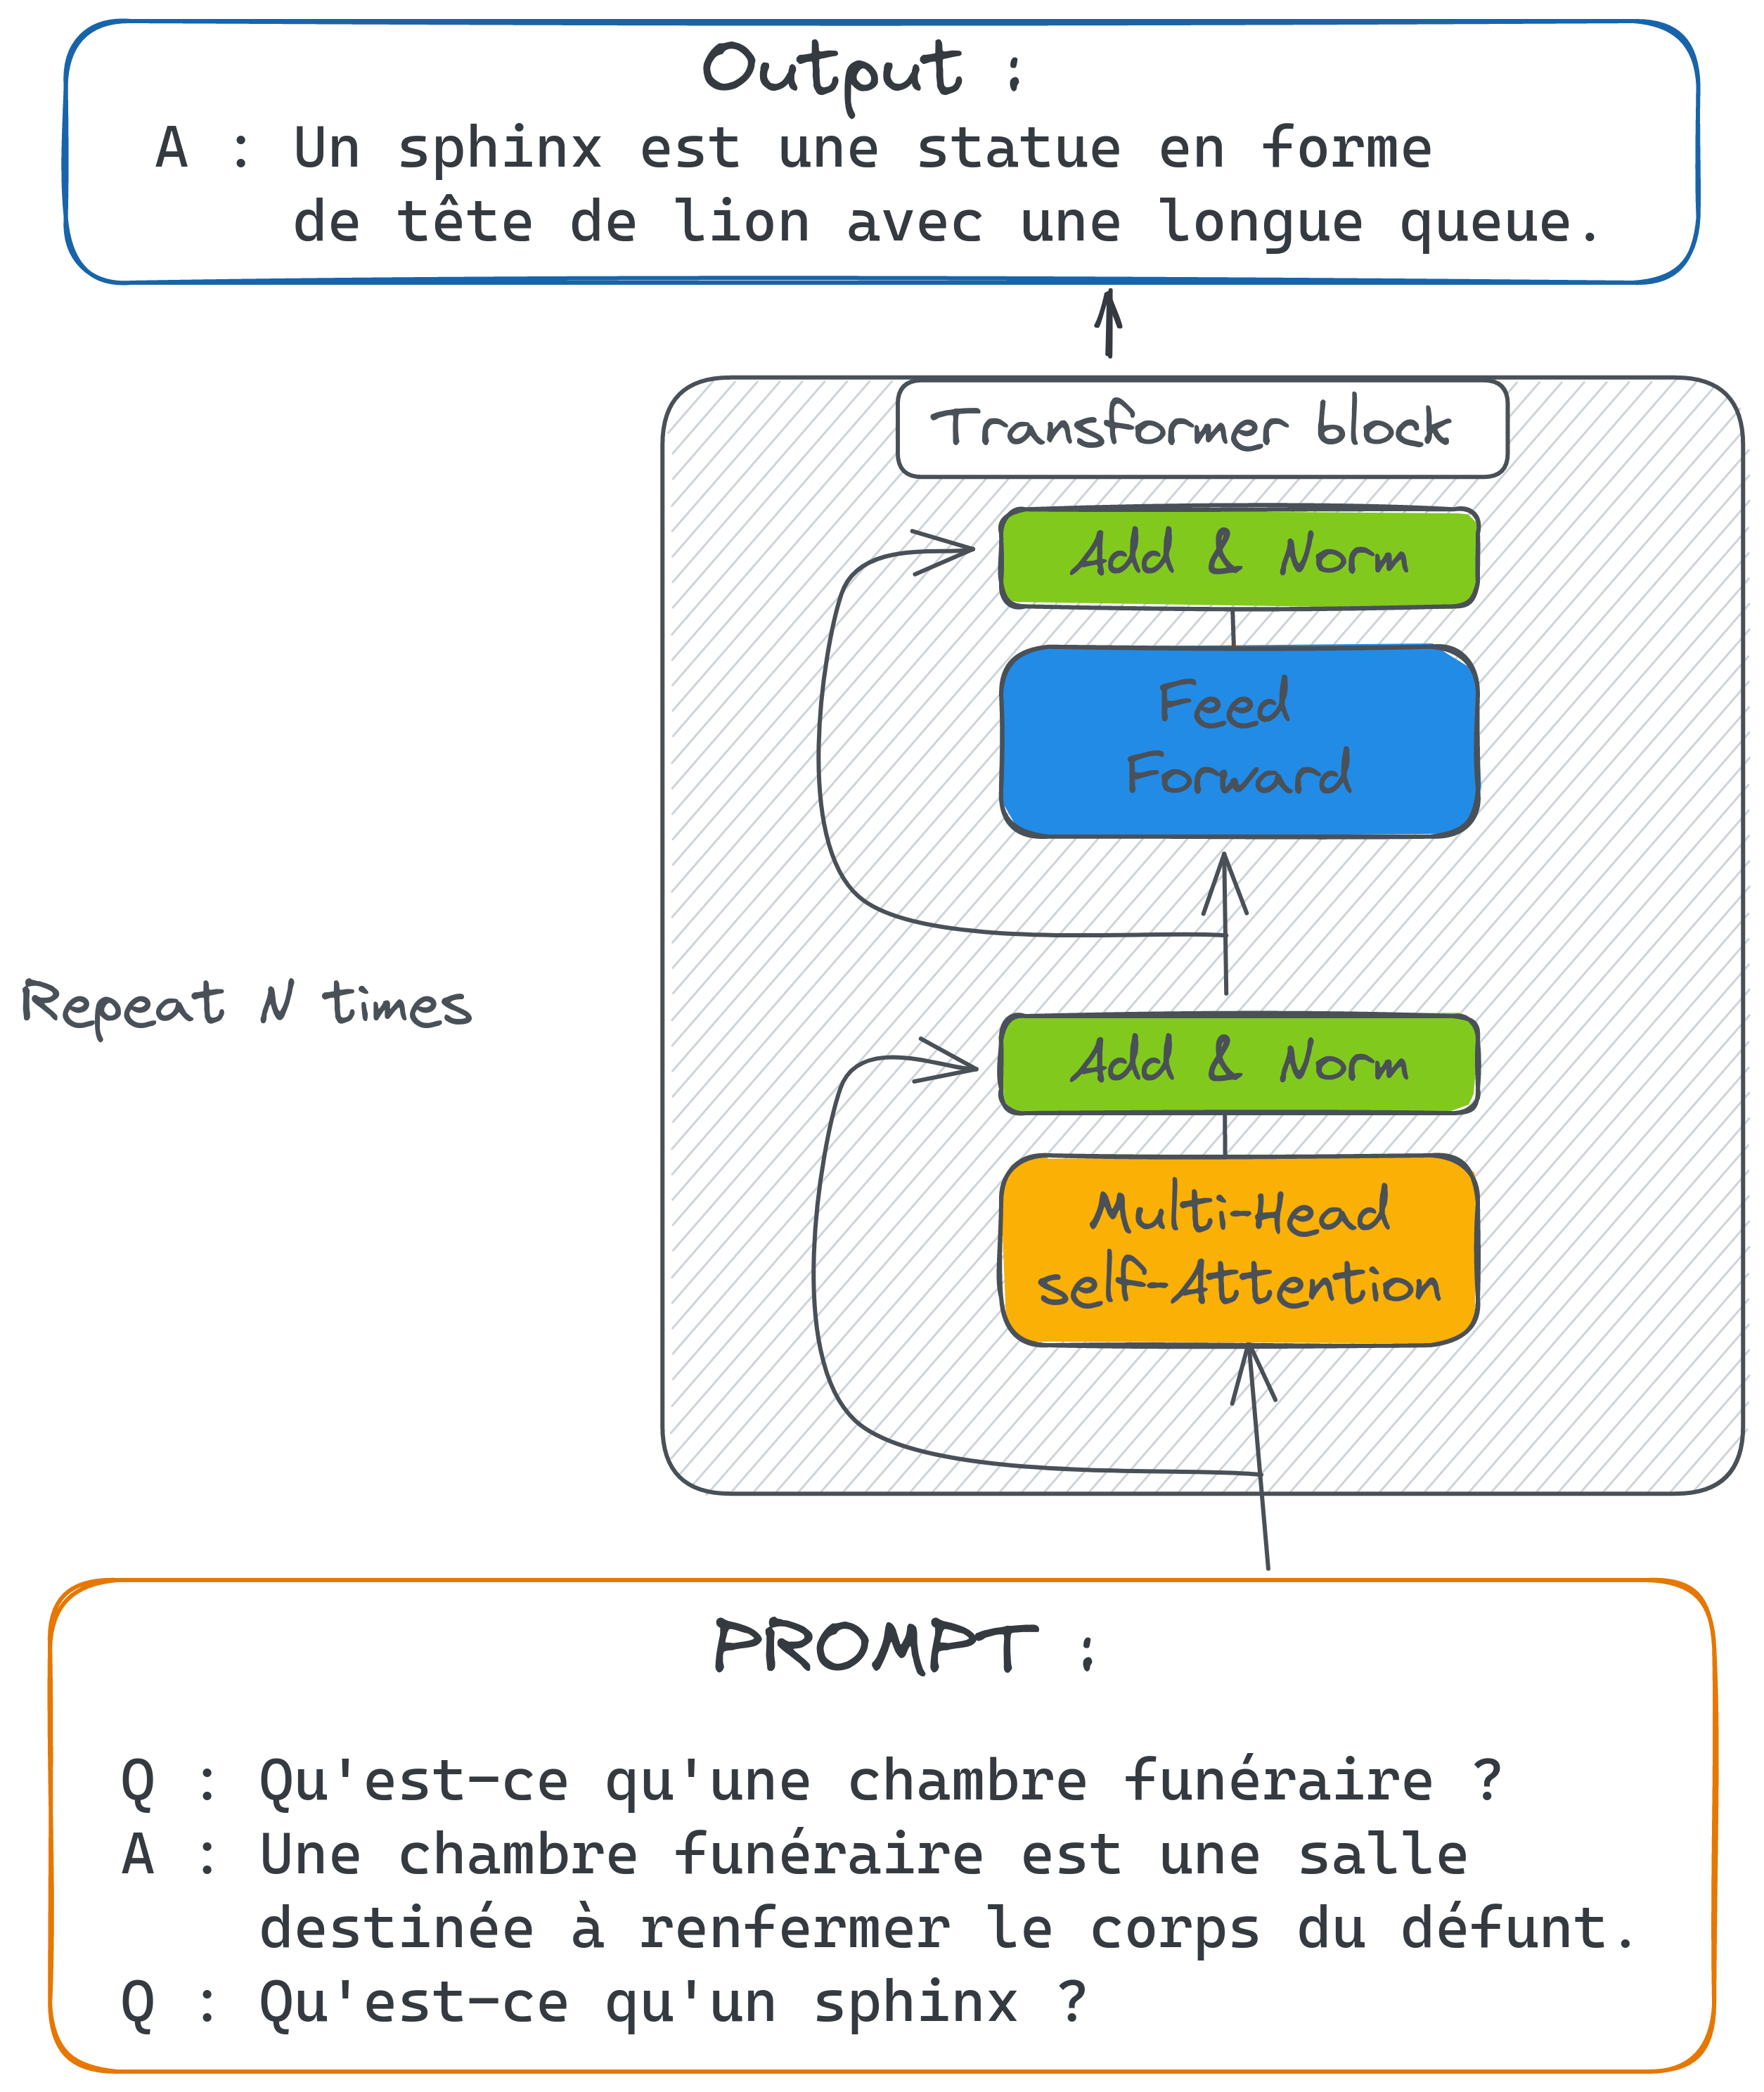
\includegraphics[width=.7\textwidth]{media/prompt-eg.png}
                \end{figure}
            \end{alertblock}
        \end{column}
    \end{columns}
\end{frame}
\begin{frame}{Instruct GPT: Step 1 Oriented generation}

    \begin{columns}
        \begin{column}{0.6\textwidth}  %%<--- here
            \begin{figure}
                \centering
                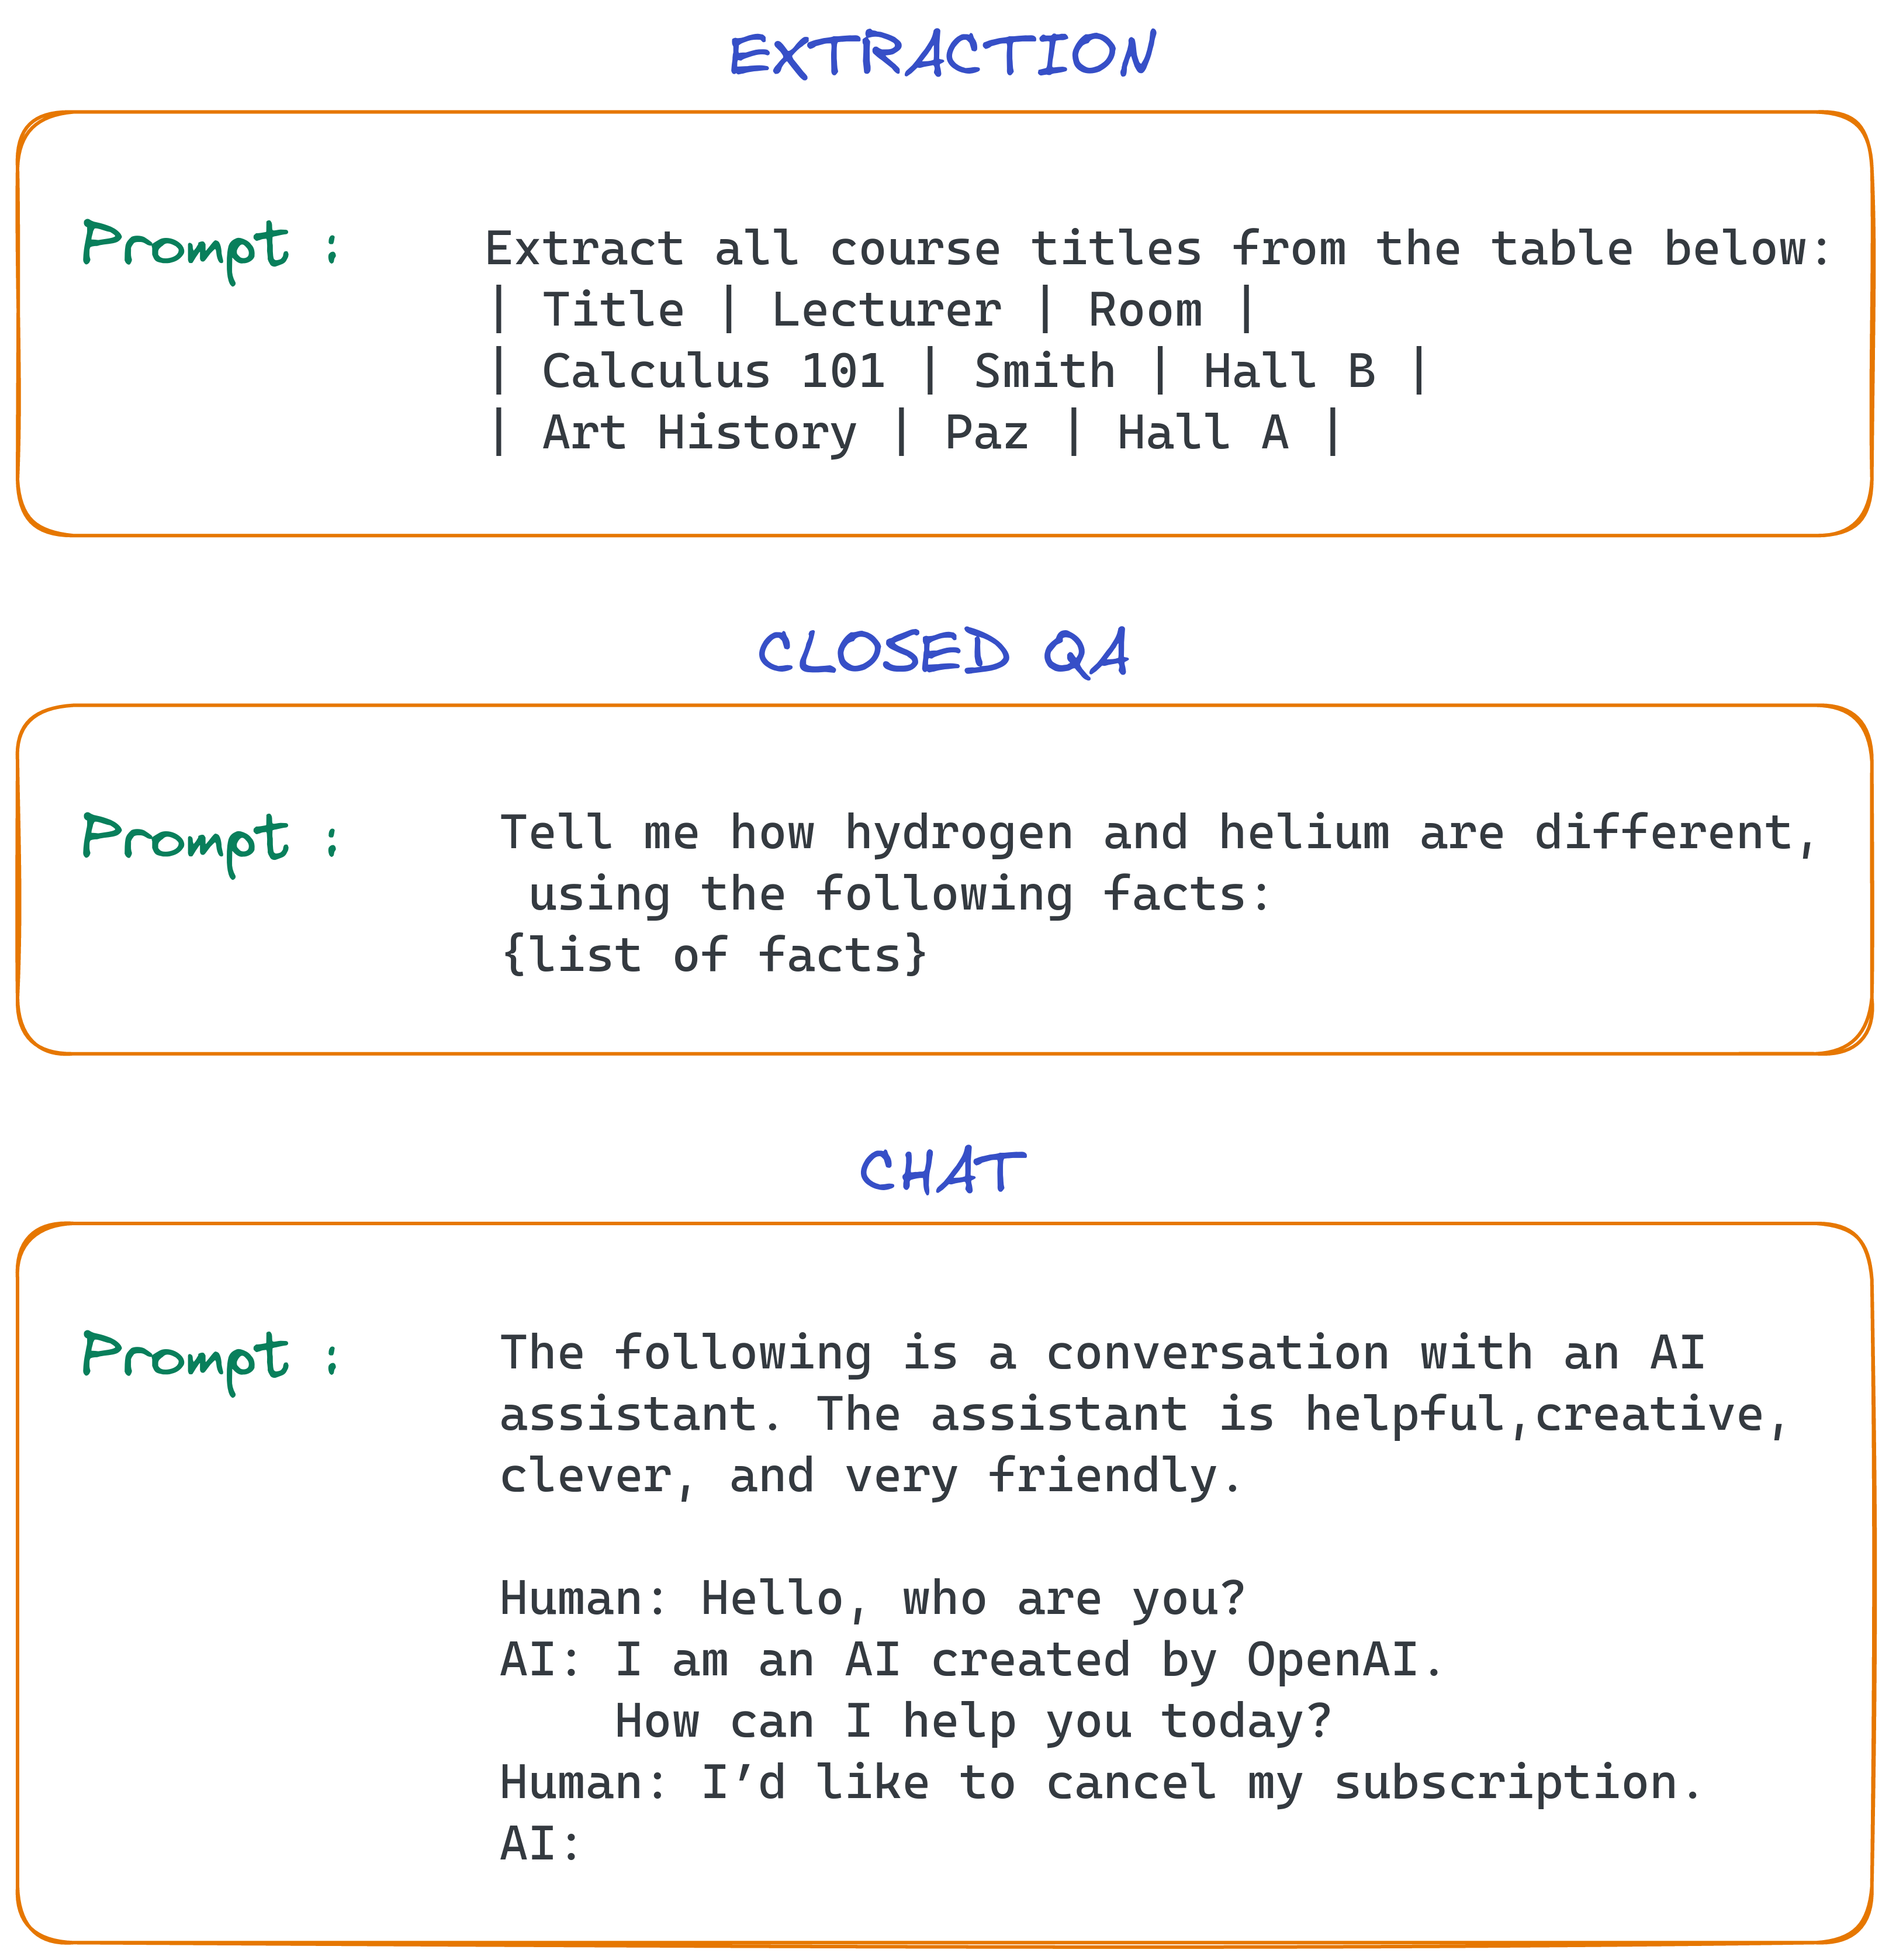
\includegraphics[width=.8\textwidth]{media/prompt_exemple.png}
                
                
            \end{figure}
        \end{column}
        \begin{column}{0.5\textwidth}
            \begin{alertblock}{Training on qualitative data}
                \begin{itemize}
                    \item Adaptation to the specific objective
                    \item Better detect the user intent (often explicitelly given)
                \end{itemize}
            
            \end{alertblock}
            \begin{alertblock}{What kind of data}
                Manually create a prompt containing : 
                \begin{itemize}
                    \item Instruction (what kind of response is expected)
                    \item Different task prompts
                \end{itemize}
                
            \end{alertblock}
        \end{column}

    \end{columns}
\end{frame}

\begin{frame}{Instruct GPT: Step 3 generalistation of preffered output}

    \begin{columns}
        \begin{column}{0.5\textwidth}
            \begin{alertblock}{Reinforcement Learning : Training a reward model}
            \footnotesize
                An other model is trained to score ``answers''
                \begin{itemize}
                    \item Human annotate ``answers preferences'' (based on different output of the model)
                    \item The Reward models is trained to rank the different answers (providing a score for generations)
                \end{itemize}

            \end{alertblock}
            \begin{alertblock}{``fine-tune'' to maximize the reward}
            \footnotesize
                \begin{itemize}
                    \item Step-1 model is trained to maximmize the reward (through a reinforcement learning algorithm named PPO) 
                    \item Keeping step-1 performances (replaying data from the step-1, not in all configurations)
                \end{itemize}

            \end{alertblock}

        \end{column}
        \begin{column}{0.6\textwidth}  %%<--- here
            \begin{figure}
                \centering
                \includegraphics[width=.8\textwidth]{media/reinforcement-instruct(1).png}
                
            \end{figure}
            \includegraphics[width=1.\textwidth]{media/instruct_gpt_formula.png}
        \end{column}
    \end{columns}
\end{frame}

\section{Evaluation}

\begin{frame}{Evaluation}
    \begin{columns}
        \begin{column}{0.5\textwidth}
            \begin{block}{Evaluate  ChitChat}
                \begin{itemize}
                    \item Evaluate generation 
                \end{itemize}
            \end{block}
            \begin{block}{Evaluate information retrieval approaches}
                \begin{itemize}
                    \item Evaluate the ranked elements
                    \item (optional) Evaluate generation 
                \end{itemize}
            \end{block}    
        \end{column}
        \begin{column}{0.5\textwidth}
            \begin{block}{Evaluate Task oriented models}
                \begin{itemize}
                    \item Evaluate NLU (classification)
                    \item Evaluate DST (classification)
                    \item Evaluate Act (classufucatuibà)
                    \item Evaluate generated answers
                \end{itemize}
            \end{block}
        \end{column}
    \end{columns}

\end{frame}

\begin{frame}{Task Oriented Systems :  Evaluate NLU/State/DA}
    \begin{block}{NLU/State/DA evaluation:}
        Does retrieved domain, intents and slots type/values correspond to what is expected ?
        \begin{itemize}
             \item \textbf{Domain, Intent} Multiclass classification (mono-label) : \\
            $$accuracy = \frac{# correctly\ predicted}{# number\ of\ predictions}$$
            \item \textbf{slot type/values} Multiclass classification (multi-label) 
                \begin{itemize}
                    \item \textbf{precision/recall} $$precision=\frac{TP}{TP+ FP}$$ $$recall=\frac{TP}{TP + FN}$$
                    \item \textbf{F1-score}  $$F1 = 2\frac{precision\times recall}{precision + recall}$$
                    
                \end{itemize}
                for non categorical slot value use exact match? /use partial match?
        \end{itemize}    
    \end{block}
\end{frame}

\begin{frame}{Evaluate Generation}
    \begin{columns}
        \begin{column}{0.6\textwidth}
            \begin{block}{Automatic evaluation}
                Evaluating simalirity with the ground truth :
                \begin{itemize}
                    \item \textbf{On tokens/words level: } Counting the number of similar words or ``N-grams'' (e.g BLEU, ROUGE, METEOR)
    
                    \item \textbf{On embeddings level} : Embed text and compare embeddings (may takes into account synonyms) such as the BERTScore\cite{}
                    \item \textbf{Entity} (between ground truth and generation)
                \end{itemize}
                
            \end{block}     
        \end{column}
        \begin{column}{0.4\textwidth}
            \begin{block}{Human evaluation}
                An example of evaluations approaches \cite{Thorleiksdttir2021UnderstandingHPb}
                \begin{itemize}
                    \item Fluency 
                    \item adequacy/informativness
                    \item grammatical correctness
                \end{itemize}
                
            \end{block}
            
        \end{column}
    \end{columns}

\end{frame}

\begin{frame}{Conversationnal Search Evaluation (Ranking)}
    \begin{block}{Evaluating ranking system}
        Does the document we produce the answer is the correct one ? 
        \begin{itemize}
            \item \textbf{Average Precision} $\frac{\sum\limits_{k=1}^n P(k)rel(k)}{nb\ relevant}$ with $rel(k) = 1$ if $k^{th}$ doc is relevant else 0 and $P(k) = \frac{|relevant \cap retrieved\_at\_k|}{retrieved\_at\_k}$
            \item \textbf{Precision@k} number of relevants items/documents in the k first retrieved documents

            \item \textbf{MRR@k} \textbf{M}ean \textbf{R}eciprocal \textbf{R}ank $\frac{1}{|Q|} \sum \limits_{q \in Q} \frac{1}{rank_q}$ where $rank_q$ is the rank of the first relevant documents retrieved
            \item \textbf{MAP} \textbf{M}ean \textbf{A}verage \textbf{P}recision 
            \item \textbf{nDCG} negative Discounted Cumulative Gain  
        \end{itemize}
    \end{block}
\end{frame}


\section{Application}

\begin{frame}{Training a NLU Systems}
    \begin{columns}
        \begin{column}{0.5\textwidth}
            \begin{block}{Data and processing}
                \begin{itemize}
                    \item ATIS/SNIPS dataset
                    \item Detecting intent 
                    \item Slot filling
                \end{itemize}
                Explore the data in BIO format, train simple classifers based on Bag-Of-Word/TF-IDF 
            \end{block}
        \end{column}
        \begin{column}{0.5\textwidth}
            \begin{block}{Create a joint Intent/slot_filling system}
            THe objective is to devllop an RNN architecture for both classification of intent (based on mean output vector) and the classification/extraction of slots in the format BIO
                \begin{itemize}
                    \item Using word embeddings train with the model
                    \item Using pretrained words embedding  
                \end{itemize}
                For the different configurations evaluate choosing relevant metrics.
            \end{block}
        \end{column}
    \end{columns}
\end{frame}

% \begin{frame}{The NLU systems}
%     \begin{columns}
%         \begin{column}{0.5\textwidth}
%             \begin{block}{The different intents}
%                 Three intents
%                 \begin{itemize}
%                     \item NONE : often greetings
%                     \item book\_restaurant : user want to book a restaurant, \textbf{describe the frame necessary for this intent}
%                     \item find\_restaurant : user want to search a restaurant \textbf{describe the frame necessary for this intent}
%                 \end{itemize}
%             \end{block}
%         \end{column}
%         \begin{column}{0.5\textwidth}
%             \begin{block}{The different slots}

%                 We will process differently categorical and non-categorical. Using classifier on the former and an extraction process for the later (classify the different tokens).
%     ['restaurant-area' 'restaurant-bookday' 'restaurant-bookpeople'
%  'restaurant-booktime' 'restaurant-food' 'restaurant-name'
%  'restaurant-pricerange']
                
%             \end{block}
%         \end{column}
%     \end{columns}
% \end{frame}

\begin{frame}[allowframebreaks]
        \frametitle{References}
        \bibliographystyle{amsalpha}
        \bibliography{biblio.bib}
\end{frame}


\end{document}
